\documentclass{article}

\usepackage{amsmath}
\usepackage{amsfonts}
\usepackage{graphicx}
\usepackage[margin=0.5in]{geometry}

\title{Energy Reconstruction Bias Studies in a Hypothetical DUNE Near Detector}
\author{Kendall Mahn, Daniel Douglas, Jacob Calcutt, Luke Pickering}

\begin{document}

\maketitle

\begin{center}
  \textit{Michigan State University}
\end{center}

%%%%%%%%%%%%%%%%%%%%%%%%%%%%%%%%%%%%%%%%%%%%%%%%%%%%
%%Plots Luke thinks that he wants to see -- may not end up in note don't take time making them pretty just stick as many as you can make in a PDF and send it on. Axis labels and titles help in huge plot dumps. Send any as soon as they are made (So I can adjust my [probably wrong] ambitions).
%
% For each of these plots, we want to be able to put some set of thresholds on,
% I haven't decided on exactly what the thresholds are yet. Did we get numbers
% from Alan? Can we look sideways at the uBooNE plots and pull an approx threshold
% out of thin air that is when the 'turn on' curve has finished (for each particle class)
% and similarly for STT.
%
% For each 1D plot, draw: No thresholds at all, GAr thresholds (for the moment can use 20 MeV KE), LAr thresholds (for the moment can use 50 MeV KE -- this may be rubbish), and higher thresholds (can use 120 MeV KE). These are for protons and charged pions, as before, never see neutrons and always see muons and pi0 (thought pi0 is probably not true for GAr... will need study).
%
% 1D histos: (flux integrated)
%% Sum of X KE in each event, where X in {proton, neutron, pi+, pi-, charged pions, pi0, proton, neutron, pi+, pi-, charged pions, pi0, proton + pi+ + pi- + pi0}
%% KE of most energetic X in each event, where X in {proton, neutron, pi+, pi-, charged pions, pi0}
%
% 2D histos: (flux divided out, as I think you are currently doing)
% E response for X. E response is KE/TE depending on the particle type -- KE for proton, TE for pion
% Sum of visible E response vs true E response for particle type.
% Add an additional X which is 'proton + pi+ + pi- + pi0 + charged lepton TE' and compare to true IS lepton energy -- this is the NOvA-style migration matrix.
%
% For each of these we want to have your great Elost/E_nu profiles as well (and as I assume that you need to make them, the 2D Elost plots that you are currently pairing with the response histos)
% The profiles can all be on the same axes per 'X' (as currently on page 5).
%
%
% So far these have all been no selection except CCInc (I saw a muon that I always see).
% we now want to do it per visible topology.
% CC0Pi, CC1Pi, CCOther. Each CCInc event should go in one of these three topologies.
% for each topology, we want to see E response 2D, ELost 2D, ELost profile, for each set of thresholds.
% We want to see the 1D Sum of X KE plot for total proton energy for CC0Pi and total pion energy for 1Pi.
%
% And just to pile it on... FHC and RHC.
%
% What do I need to do/provide? As per the previous plan, I agree that we should look at one generator
% and make every plot we think might be worth having, and then can expand on the most interesting ones
% with other generators.
%
% This might sound like a lot, I don't expect it over night and it may not all be neccessary, so we should update what we want as some of them get made. I think showing some reco-topology selections is important soon, and looking at the 1D particle energy spectra. I'm not sure how you're currently making plots and how abstracted it is (i.e. easy to expand to making millions of plots with just different TTree::Draw selections), if it is currently labour intensive we can try and work out a way to make it not so (I have some tools in this regard... but from the rate of pretty plots you guys send, it seems that, so do you!)
%%%%%%%%%%%%%%%%%%%%%%%%%%%%%%%%%%%%%%%%%%%%%%%%%%%%

\section{Introduction}

We've been working on understanding the response and reconstruction abilities of three proposed designs for the near detector of the Deep Underground Neutrino Experiment (DUNE).  The designs considered in our studies have been:

\begin{itemize}
\item Fine-Grained Tracker (FGT)
\item Liquid Argon Time Projection Chamber (LAr TPC)
\item Gaseous Argon Time Projection Chamger (GAr TPC)
\end{itemize}

Of major interest for the scientific goals of a near detector in an experiment such as DUNE is the ability to detect and reconstruct the energy of a neutrino which interacts in the detector.  Being able to measure the energy spectrum of neutrinos at the near detector with very little uncertainty allows us to better understand the flux at the far detector, after it has undergone some oscillation.  It is our belief that a poor estimation of this flux (mainly by a systematic bias on the measured flux) can contribute to the rate of false positive measurements of various oscillation parameters (notably, $\delta_{\mathrm{CP}}$).
%Jake: I'd change the wording of this. Maybe saying that we get a *biased* measurement of the oscillation parameters is more accurate here and applies more generally to the rest of the parameters. After that, then saying that this could result in a false positive measurement of dcp would fit better to me. (Kendall, Luke, Minerba thoughts?)


The studies presented here are much broader and focus on the energy estimation.  The two largest contributions to the uncertainty in flux measurement are

\begin{itemize}
\item Detector efficiency
\item Reconstruction error
\end{itemize}

\section{Efficiency}

The efficiency of each event selection is defined here in terms of the migration of events from one true topology to several reconstructed topologies.  In the case of no threshold, every topology can be reconstructed correctly and the efficiency is 100\%.  

\subsection{FHC}

\subsubsection{CC0Pi}

True CC0Pi events are always reconstructed as CC0Pi events.

\begin{center}

\includegraphics[width=0.245\textwidth]{plots/efficiency/CC0Pi_FHC_No_Threshold.pdf}
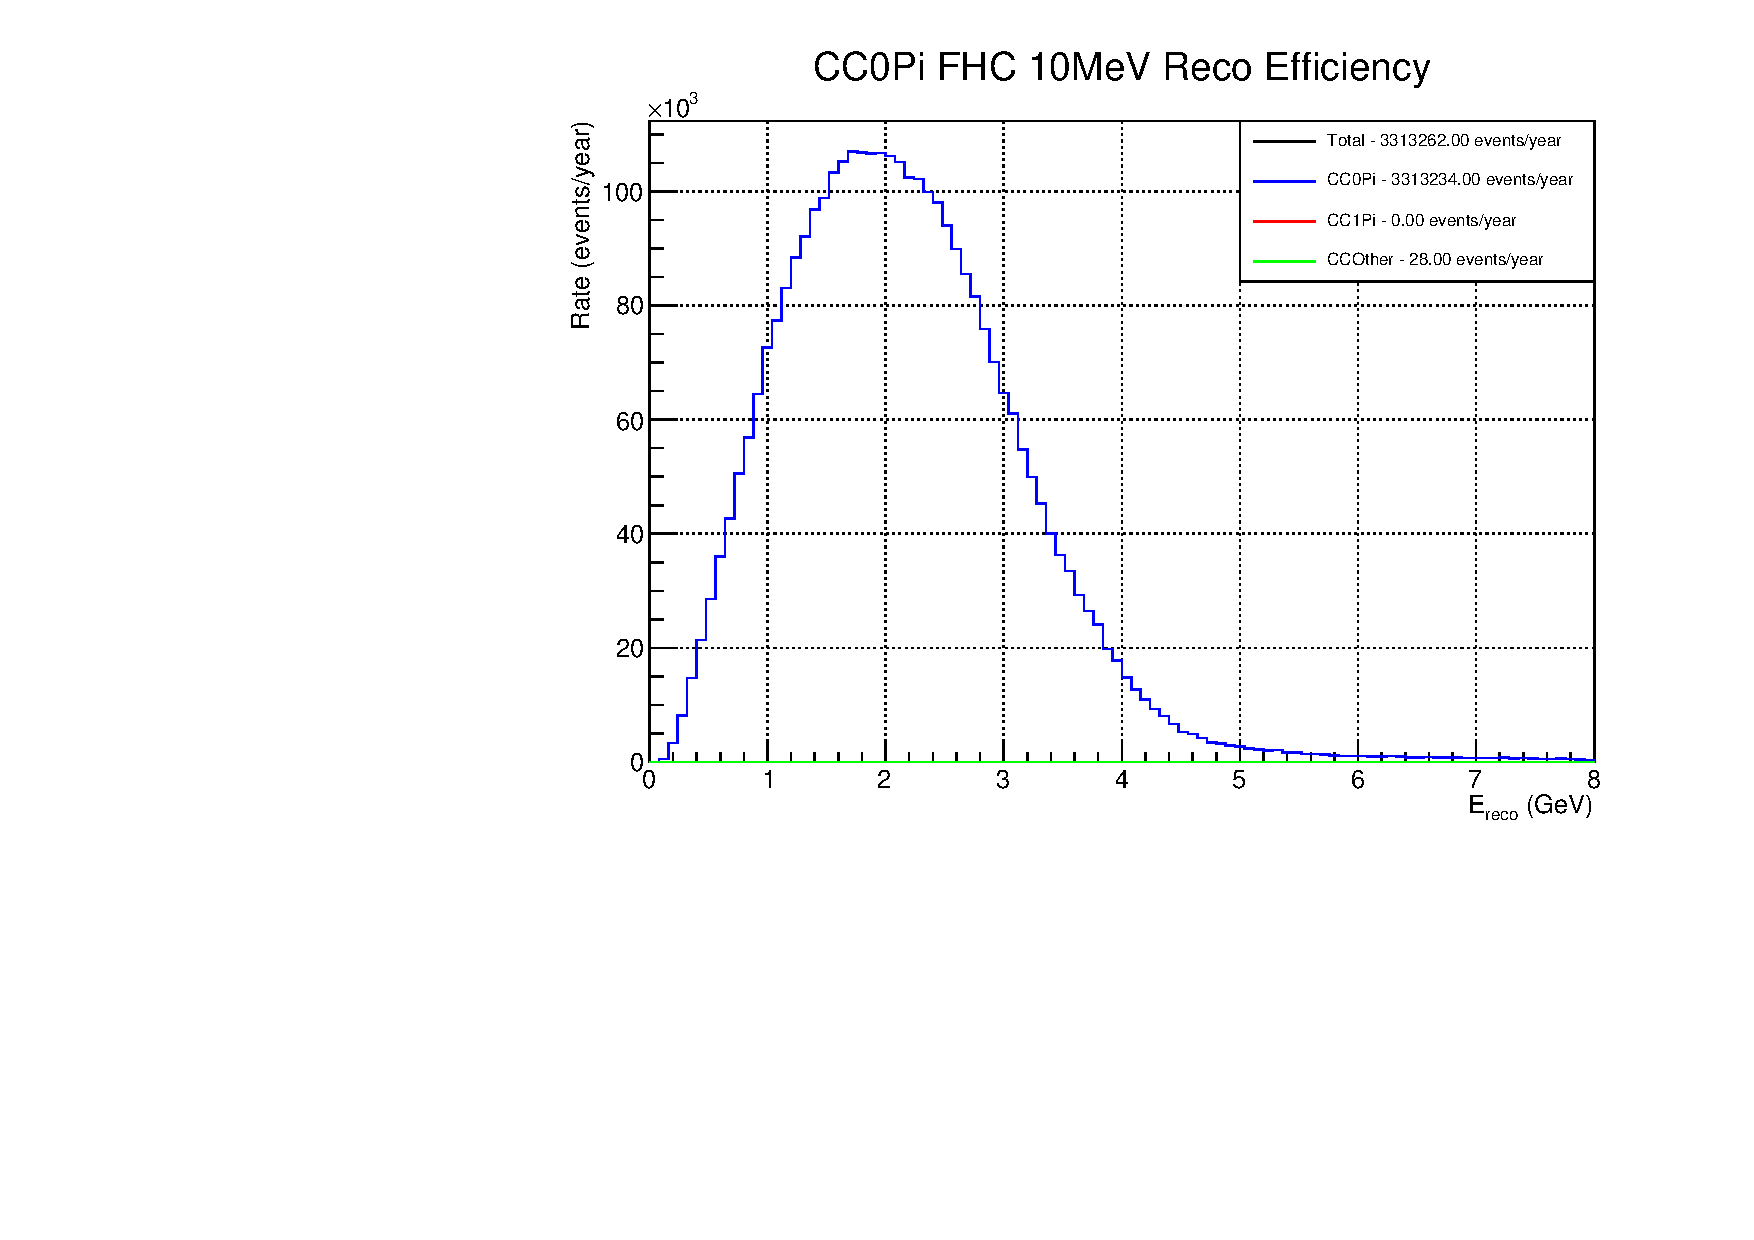
\includegraphics[width=0.245\textwidth]{plots/efficiency/CC0Pi_FHC_10MeV.pdf} 
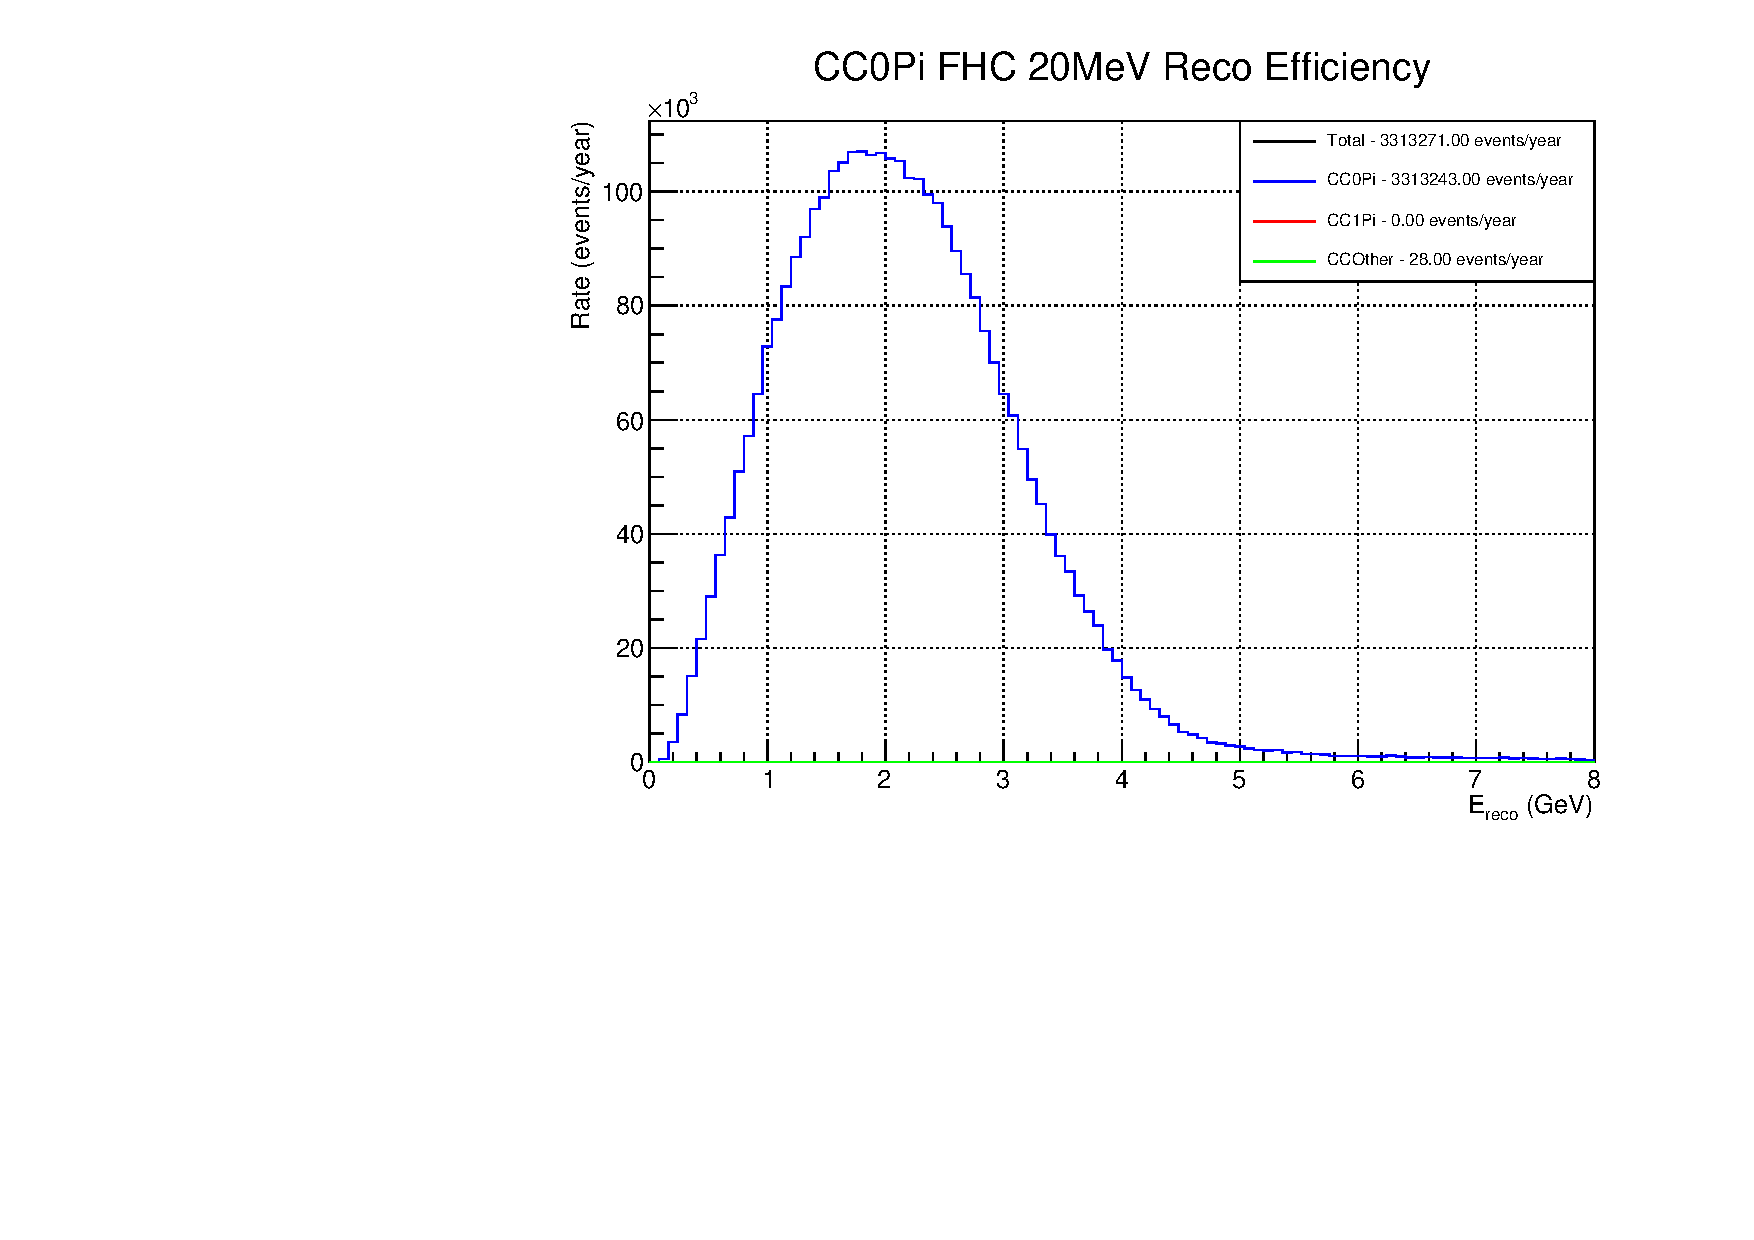
\includegraphics[width=0.245\textwidth]{plots/efficiency/CC0Pi_FHC_20MeV.pdf}
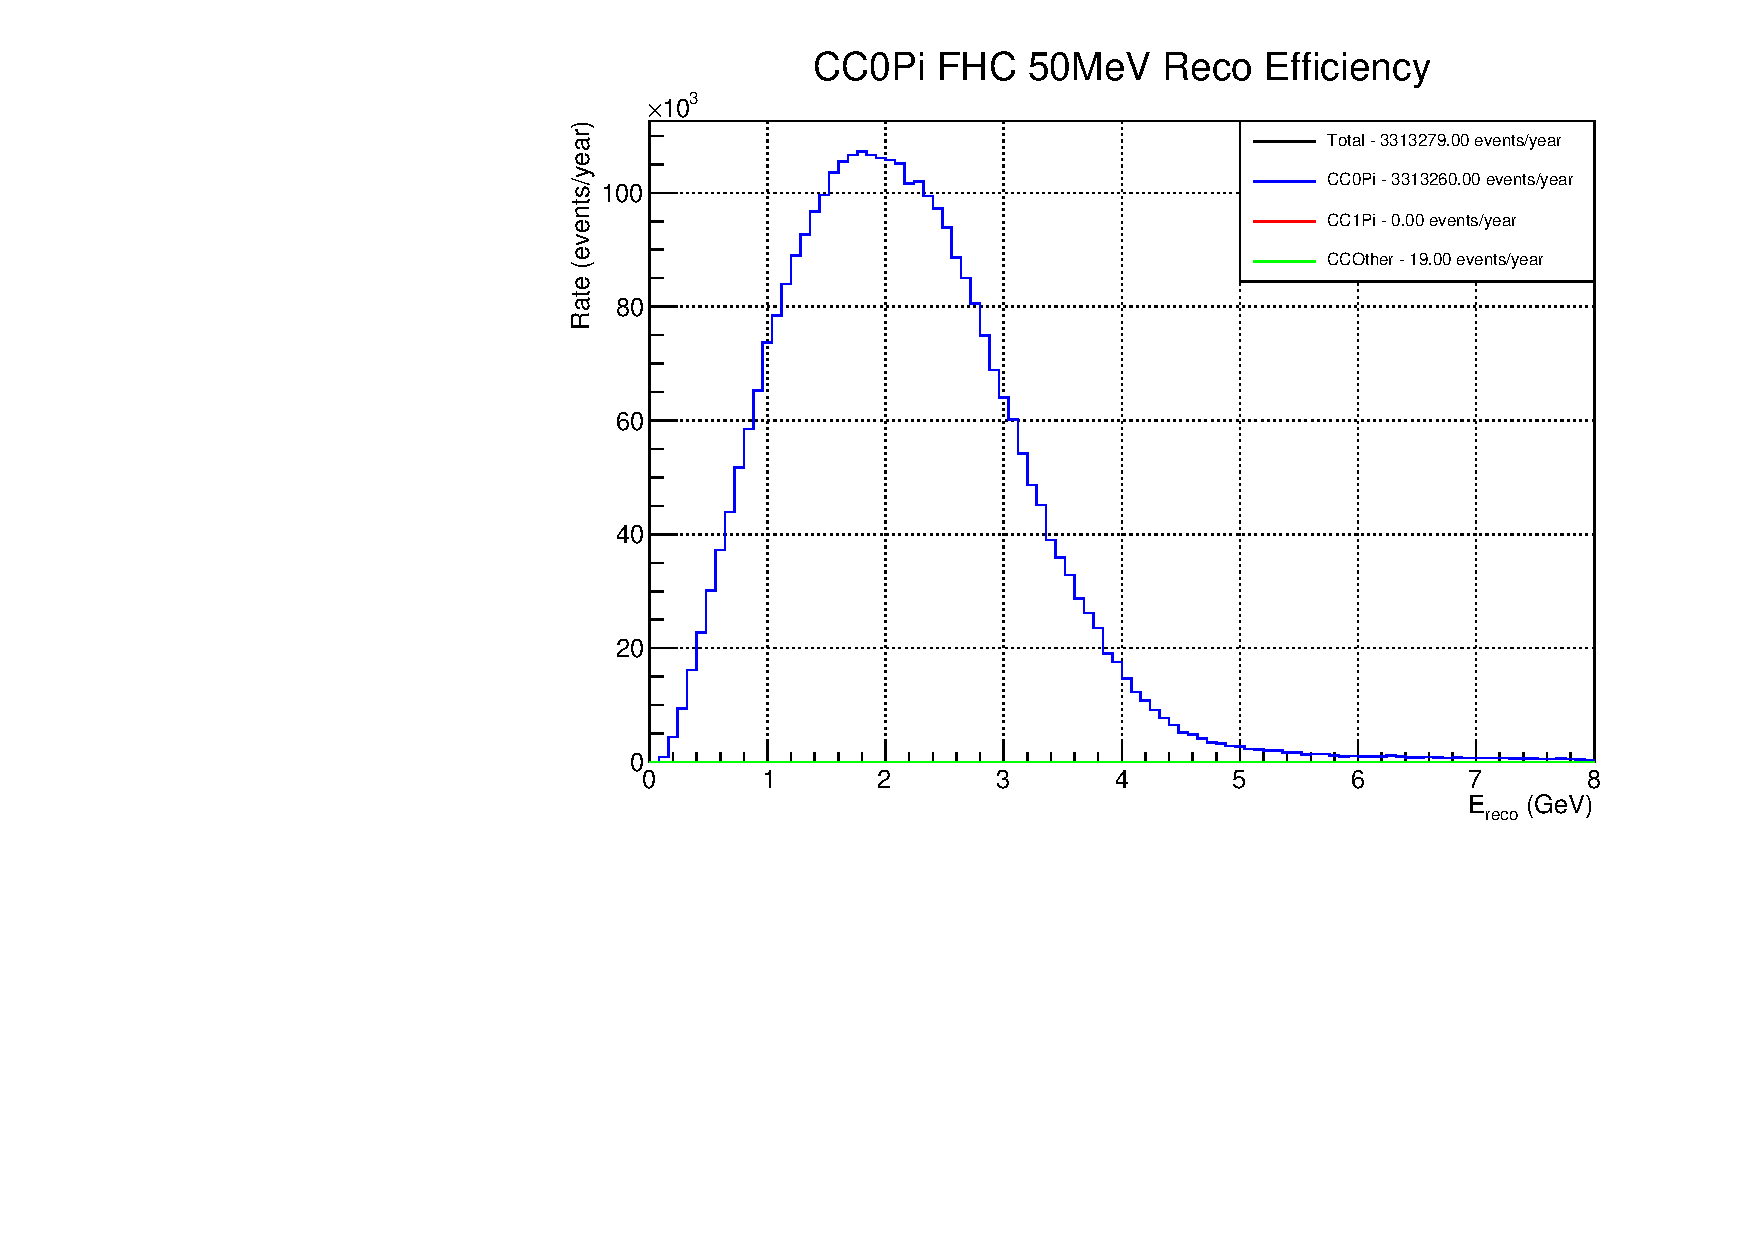
\includegraphics[width=0.245\textwidth]{plots/efficiency/CC0Pi_FHC_50MeV.pdf}

\end{center}

\subsubsection{CC1Pi}

True CC1Pi events will be reconstructed as CC0Pi events if the pion is beneath the threshold.

\begin{center}

\includegraphics[width=0.245\textwidth]{plots/efficiency/CC1Pi_FHC_No_Threshold.pdf}
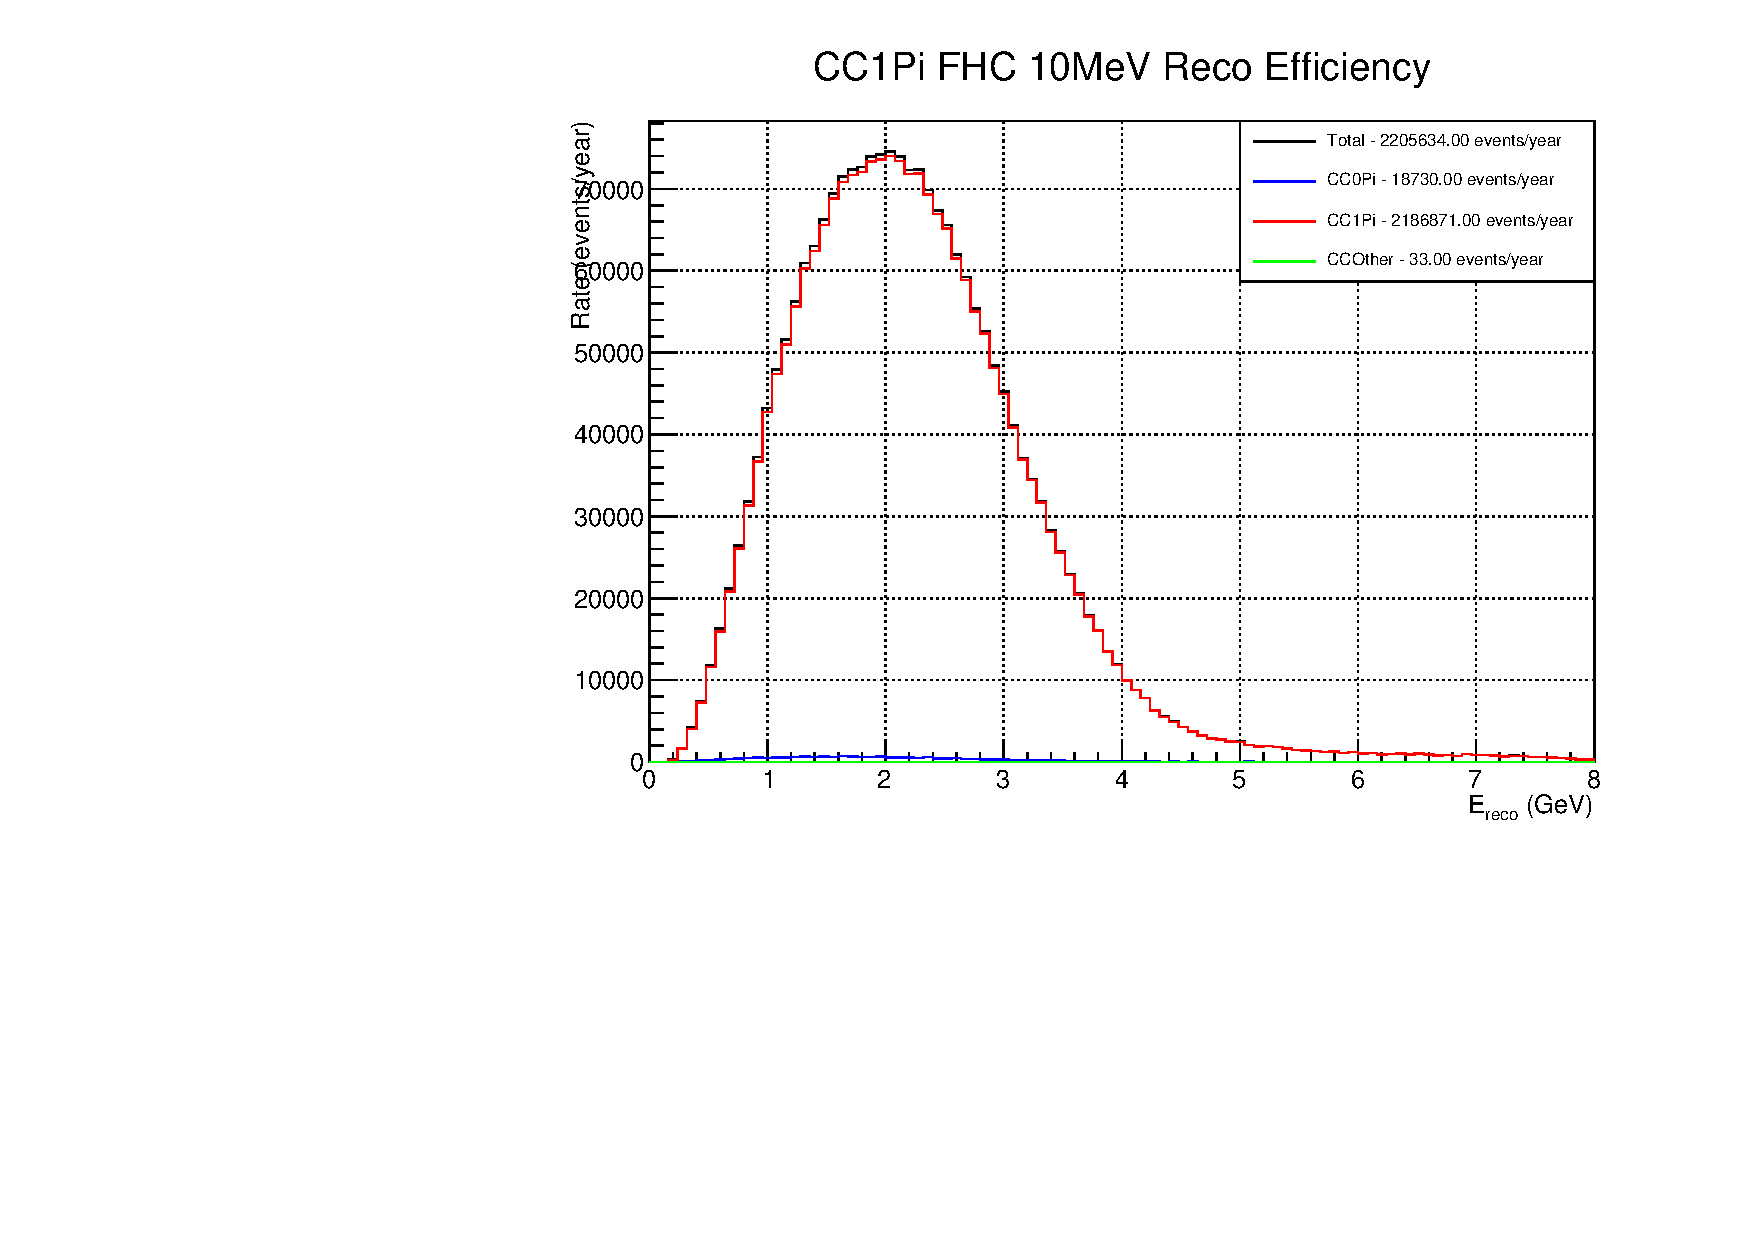
\includegraphics[width=0.245\textwidth]{plots/efficiency/CC1Pi_FHC_10MeV.pdf} 
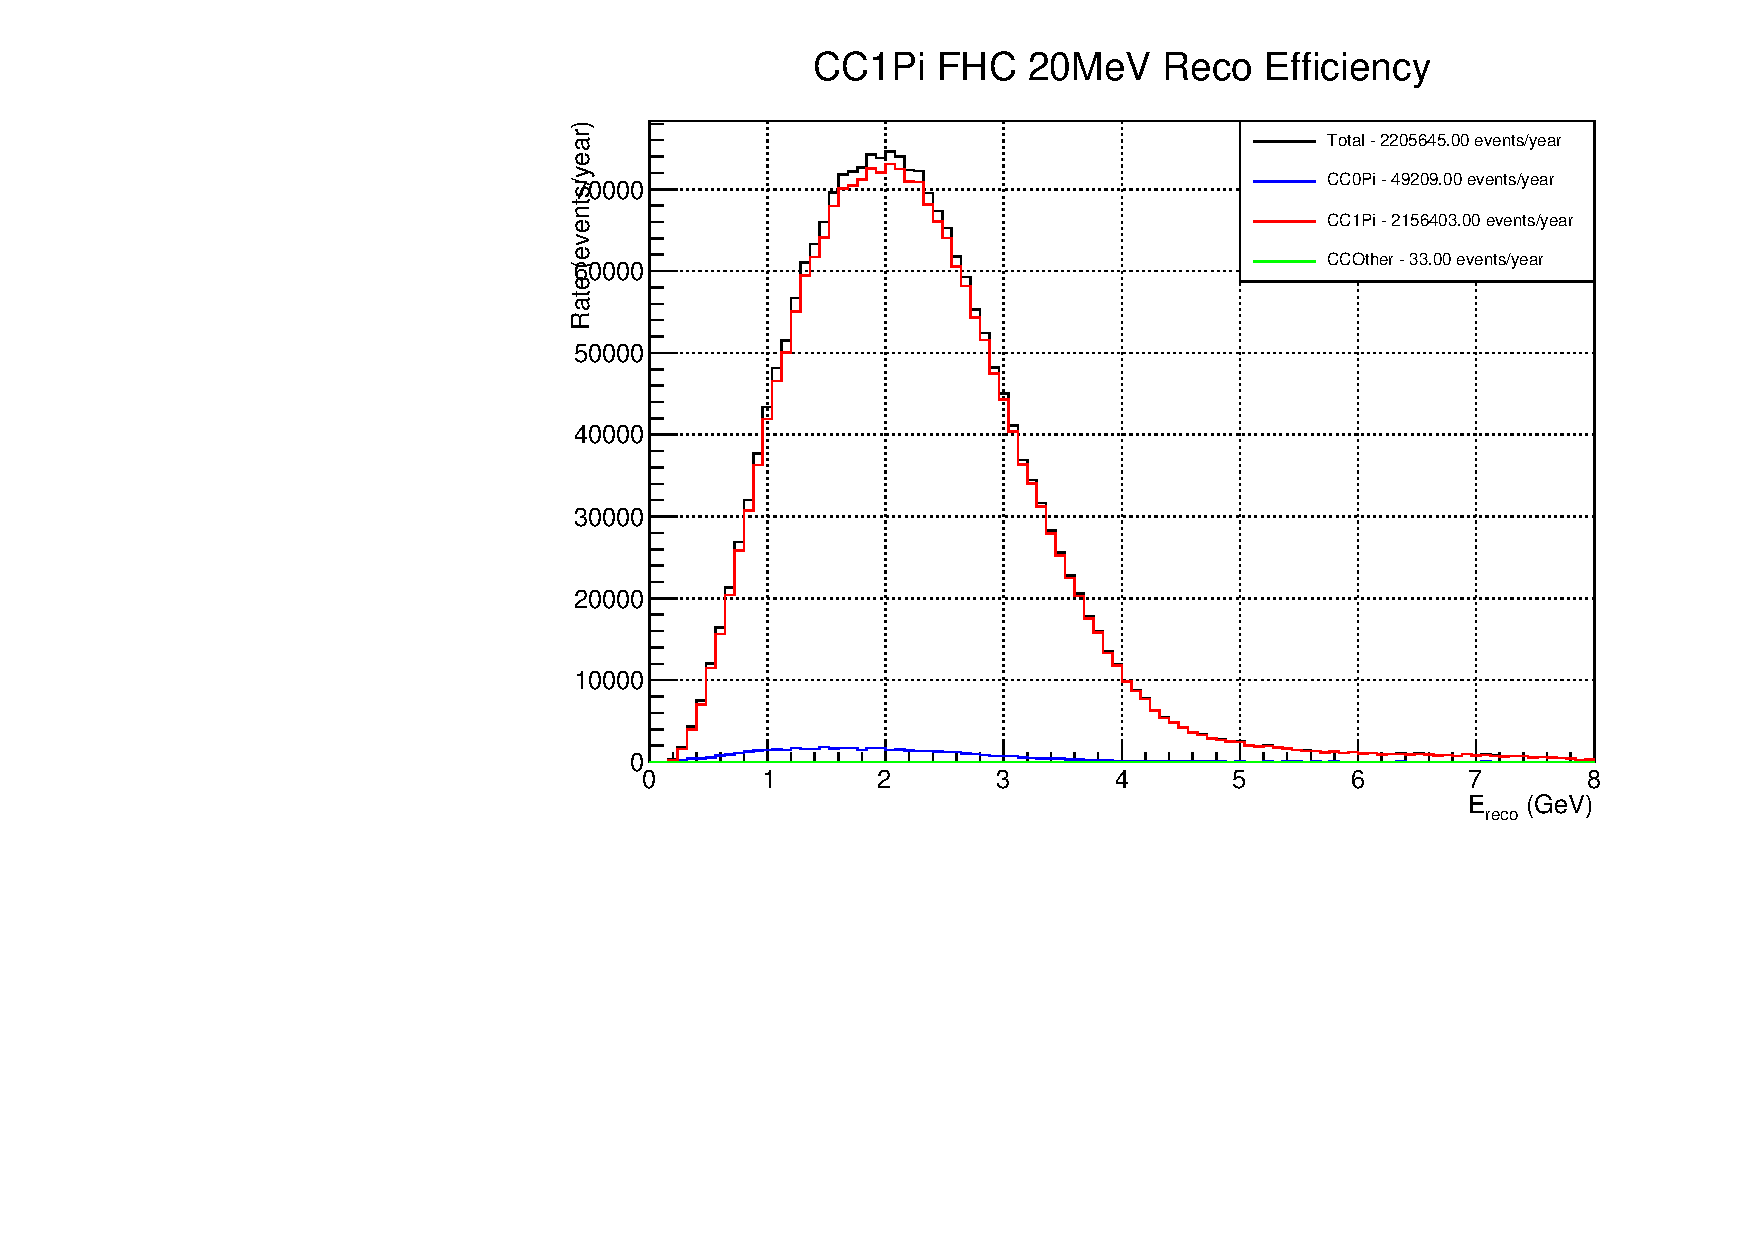
\includegraphics[width=0.245\textwidth]{plots/efficiency/CC1Pi_FHC_20MeV.pdf}
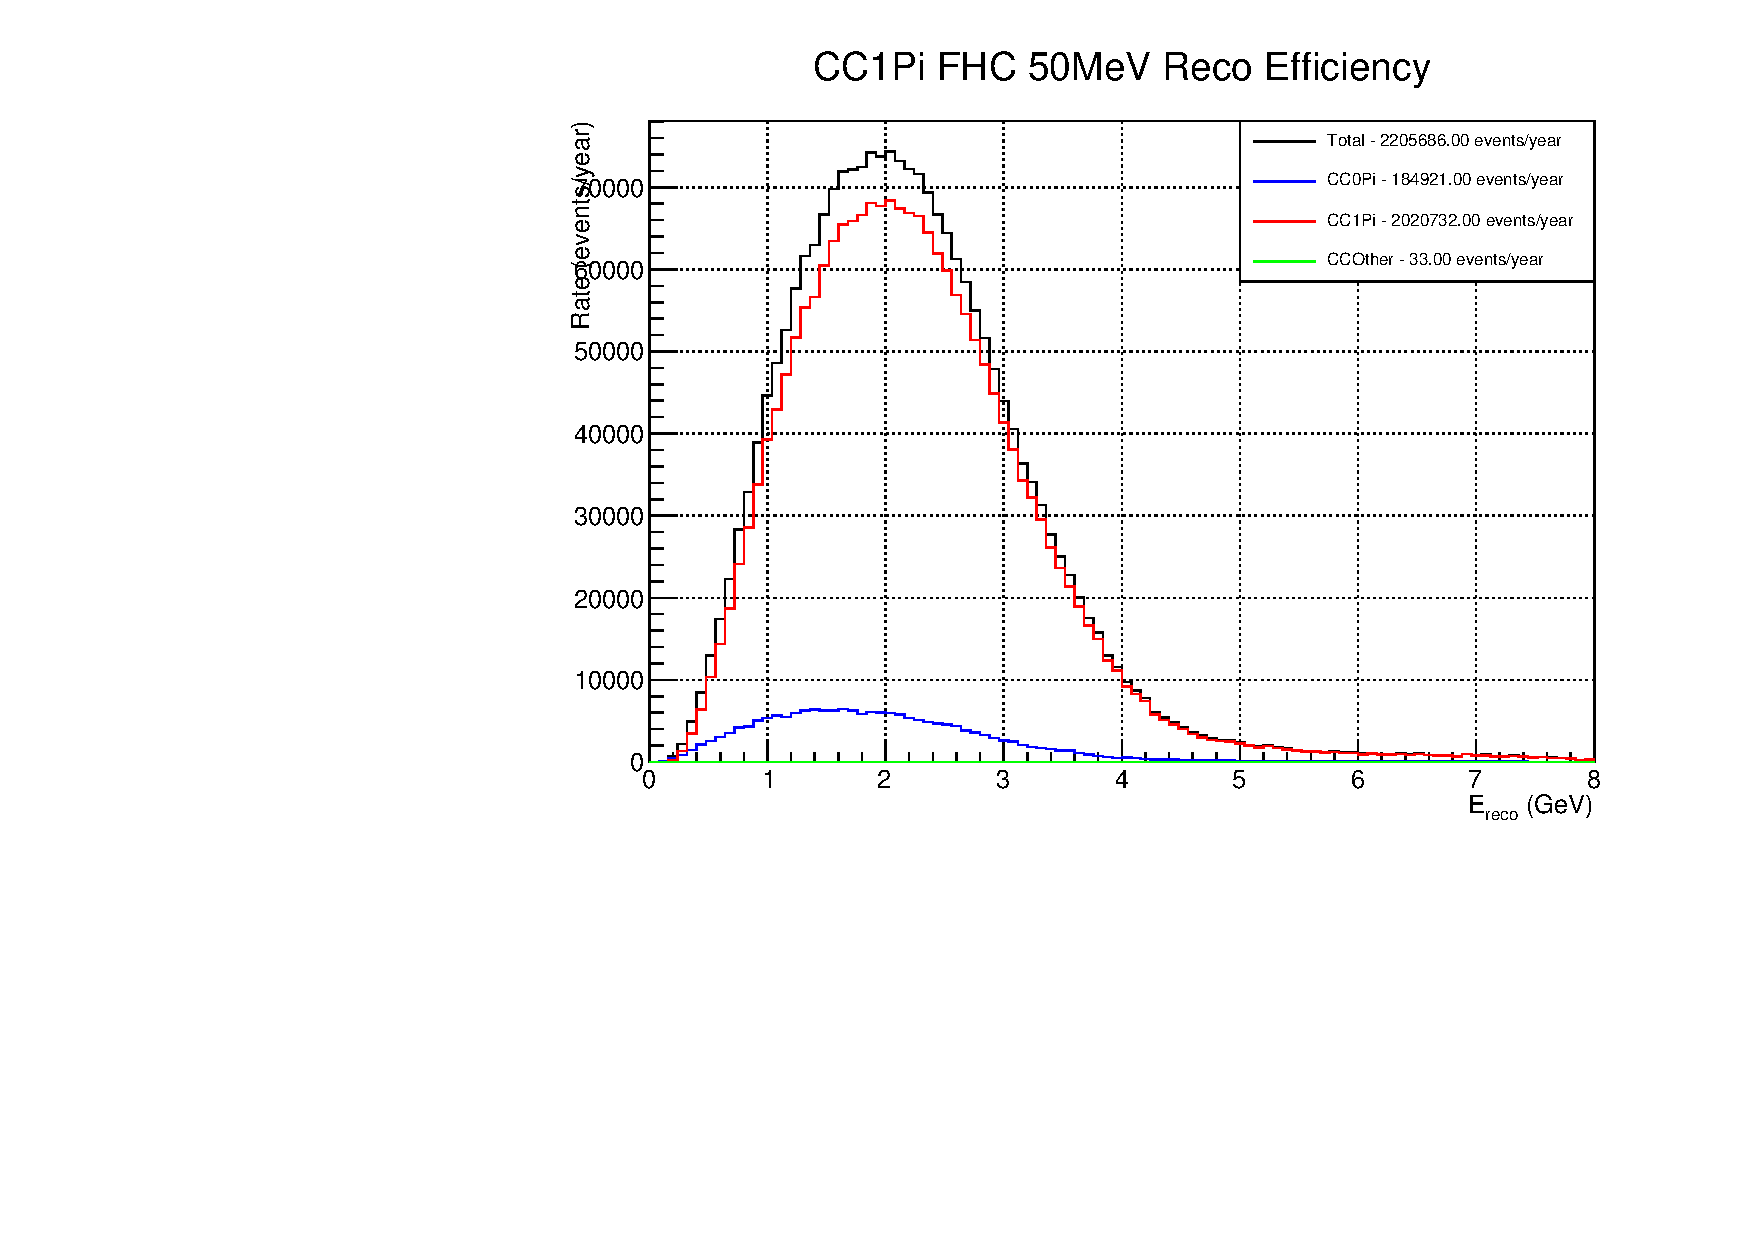
\includegraphics[width=0.245\textwidth]{plots/efficiency/CC1Pi_FHC_50MeV.pdf}

\end{center}

\subsubsection{CCOther}

True CCOther events can be reconstructed as CC1Pi or CC0Pi depending upon how many pions are beneath the tracking threshold.

\begin{center}

\includegraphics[width=0.245\textwidth]{plots/efficiency/CCOther_FHC_No_Threshold.pdf}
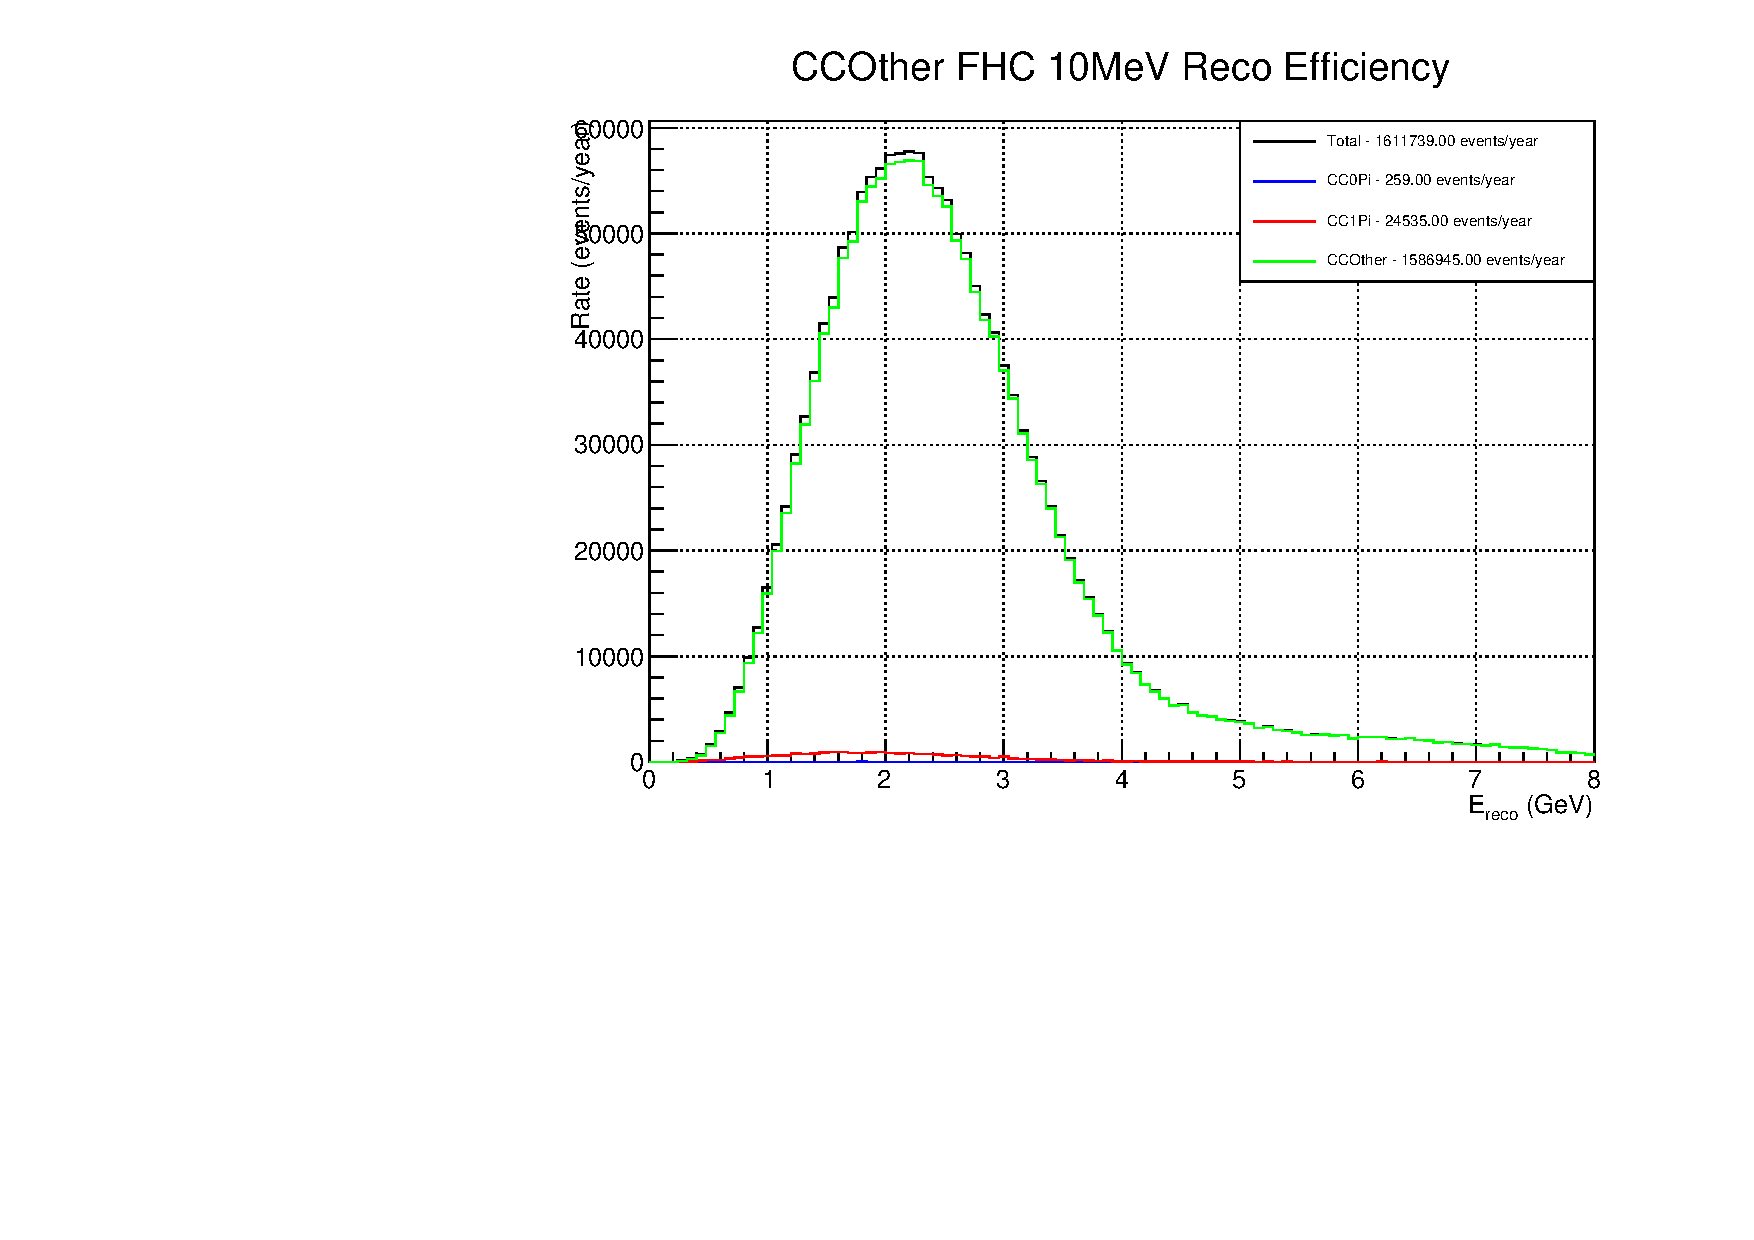
\includegraphics[width=0.245\textwidth]{plots/efficiency/CCOther_FHC_10MeV.pdf} 
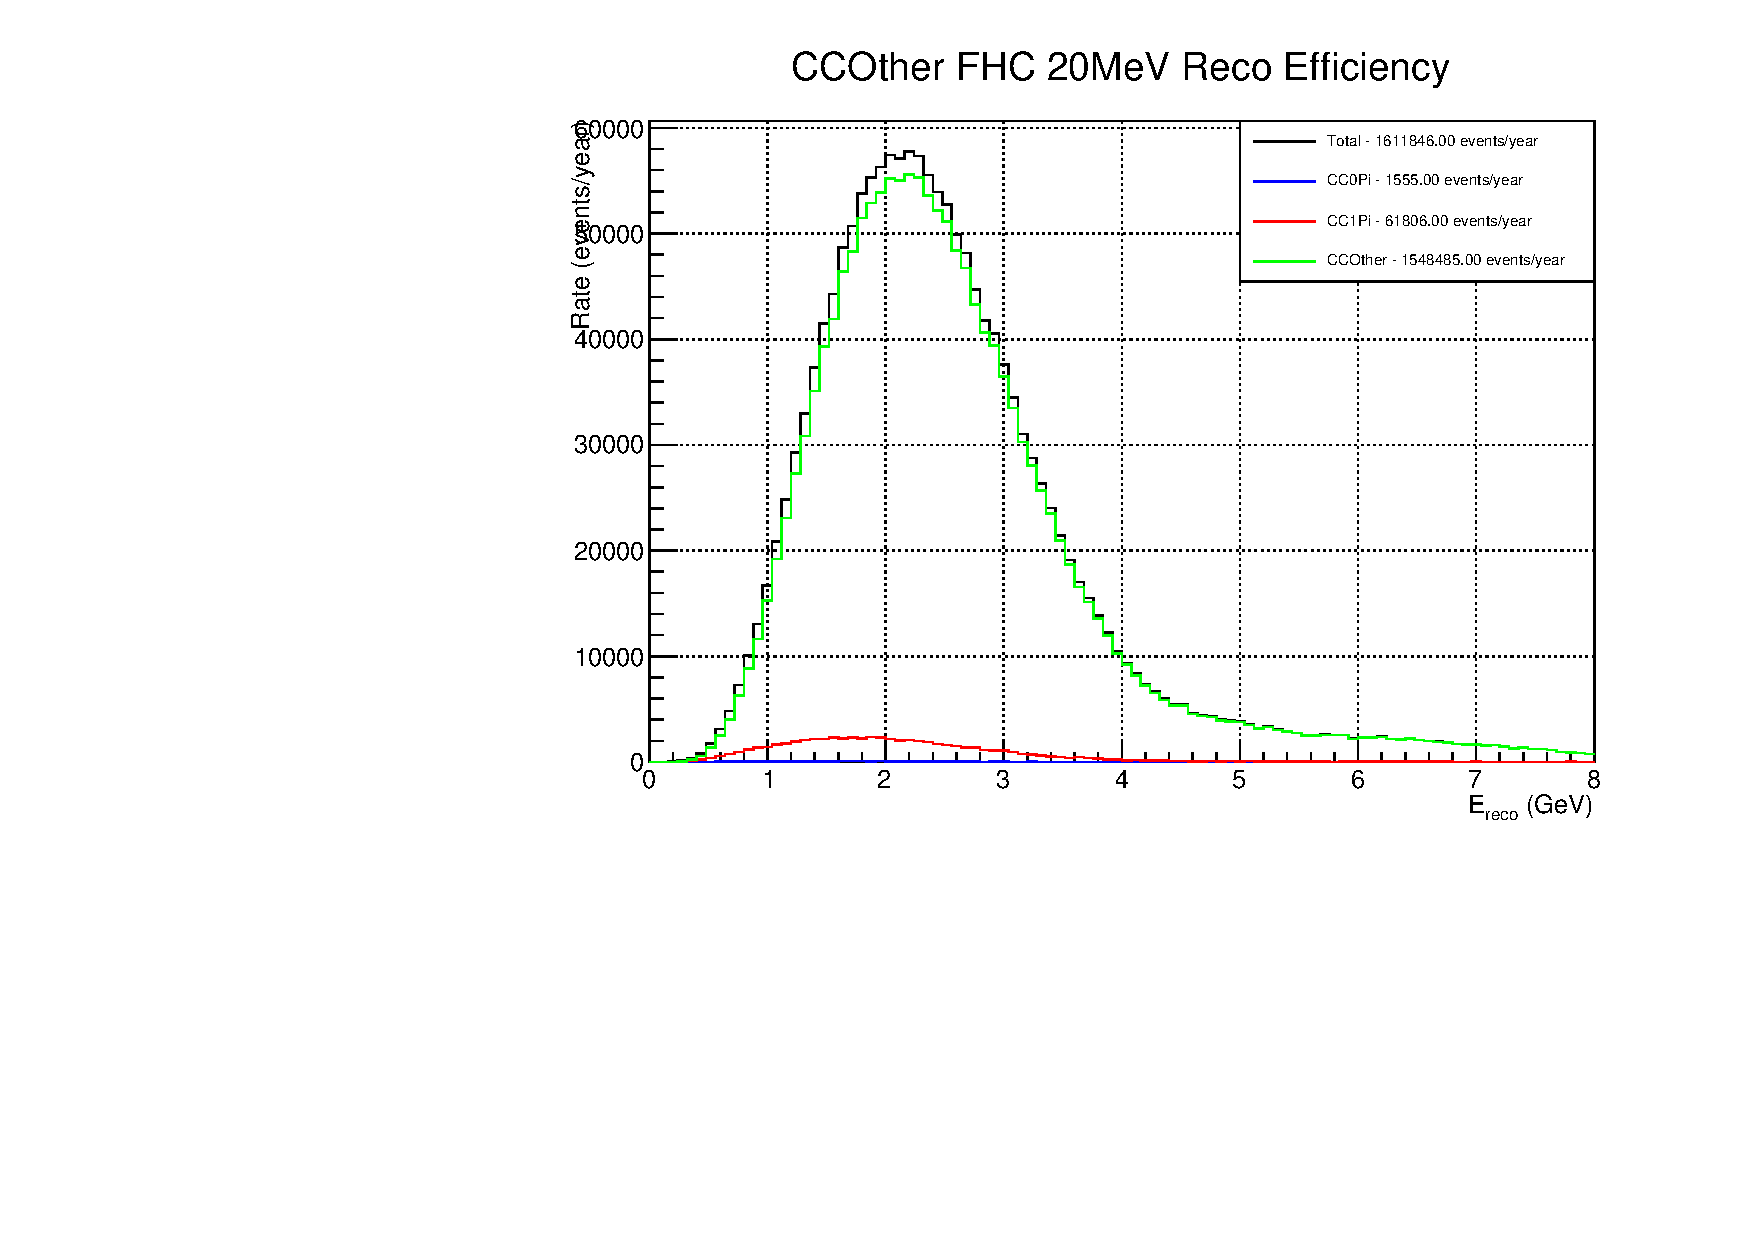
\includegraphics[width=0.245\textwidth]{plots/efficiency/CCOther_FHC_20MeV.pdf}
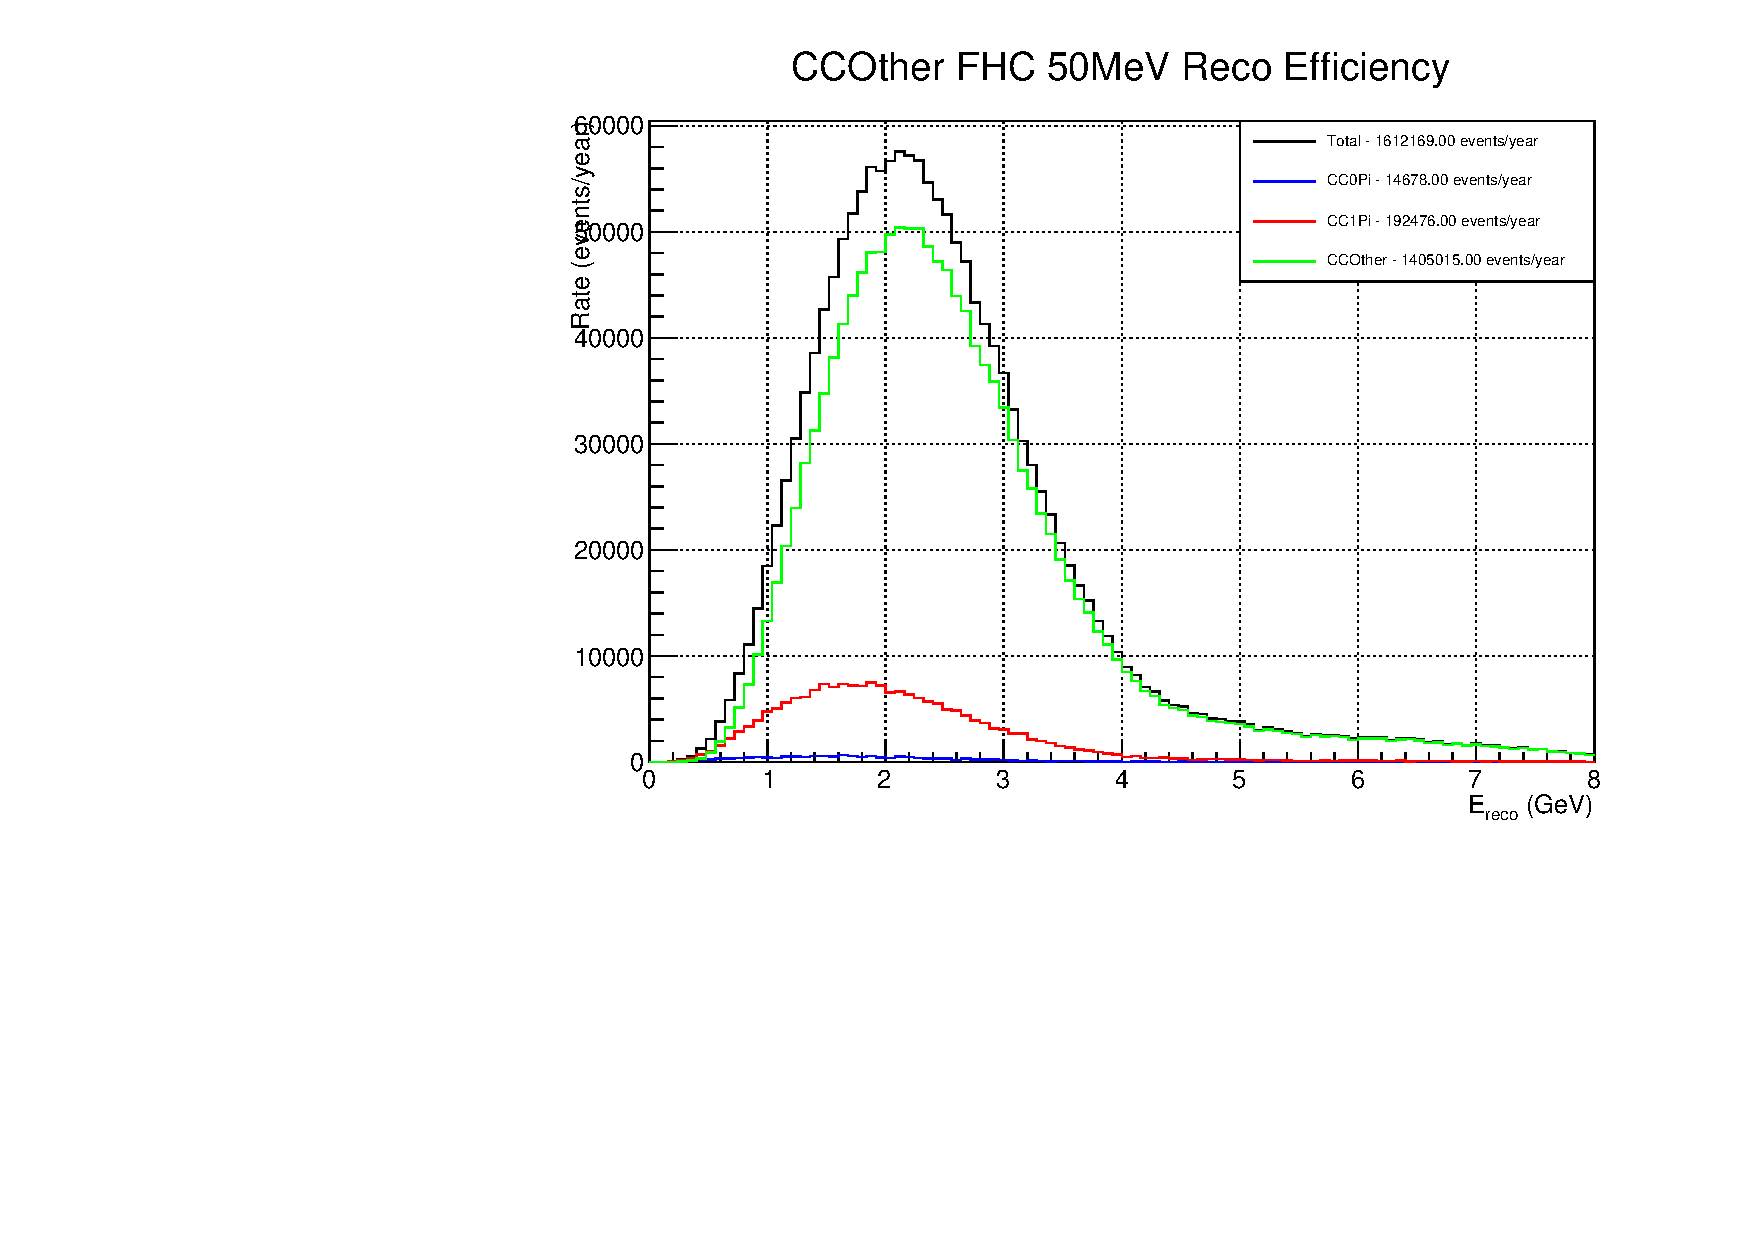
\includegraphics[width=0.245\textwidth]{plots/efficiency/CCOther_FHC_50MeV.pdf}

\end{center}


\subsection{RHC}

\subsubsection{CC0Pi}

\begin{center}

\includegraphics[width=0.245\textwidth]{plots/efficiency/CC0Pi_RHC_No_Threshold.pdf}
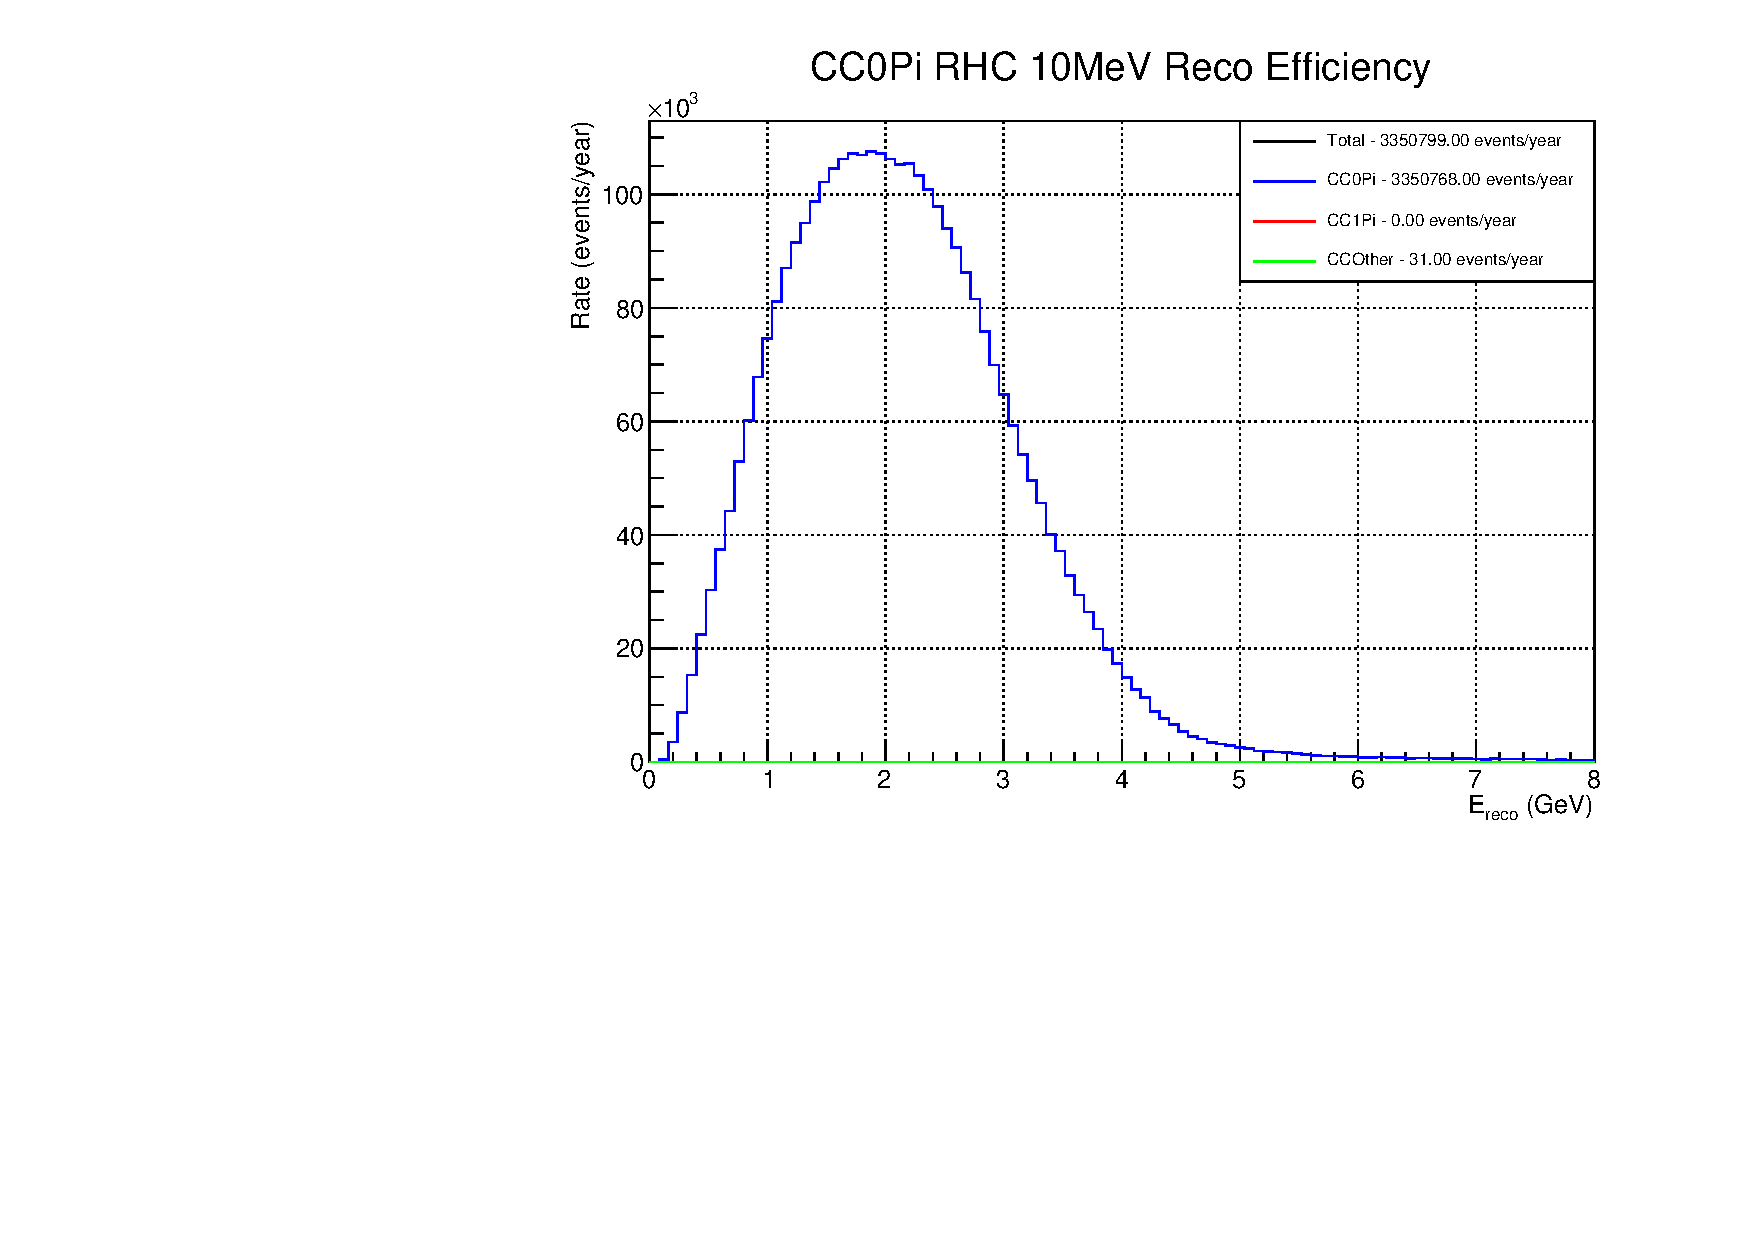
\includegraphics[width=0.245\textwidth]{plots/efficiency/CC0Pi_RHC_10MeV.pdf} 
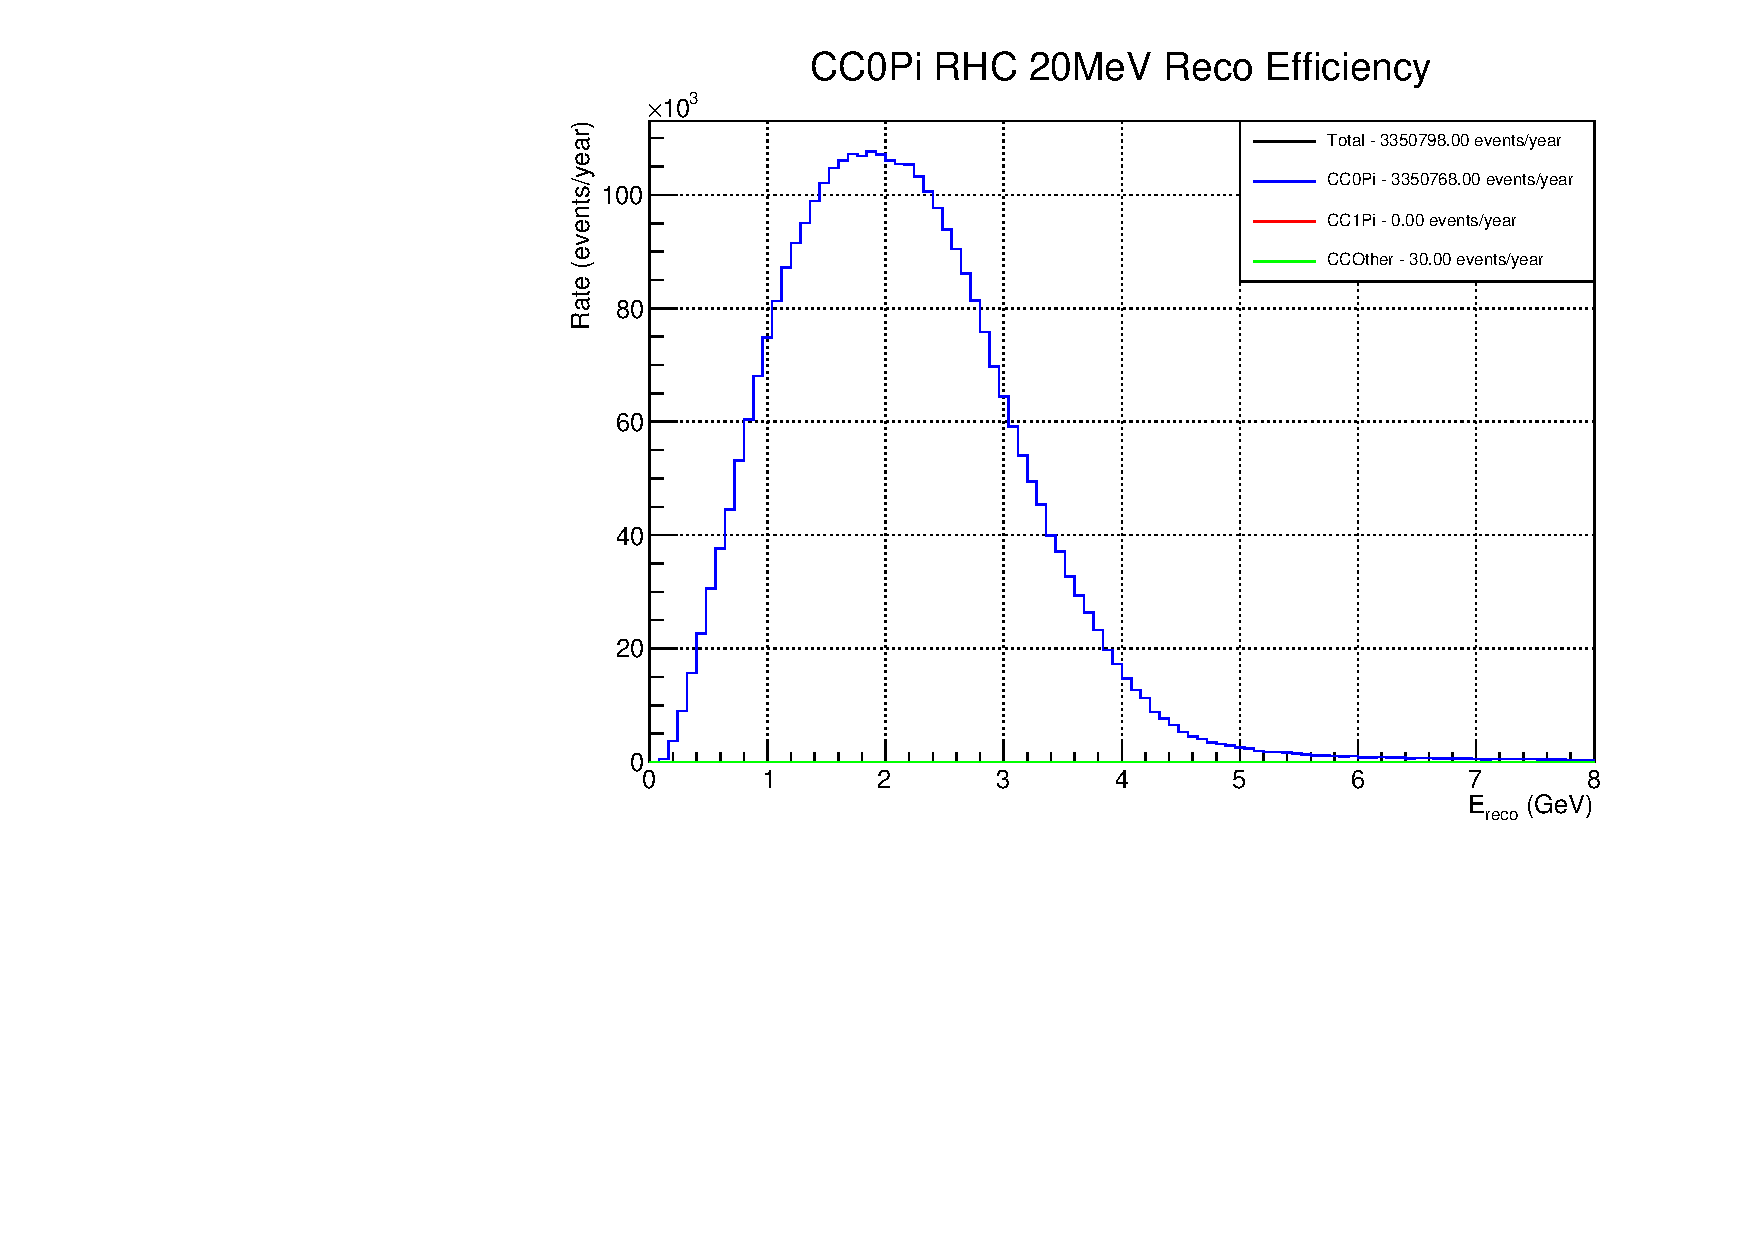
\includegraphics[width=0.245\textwidth]{plots/efficiency/CC0Pi_RHC_20MeV.pdf}
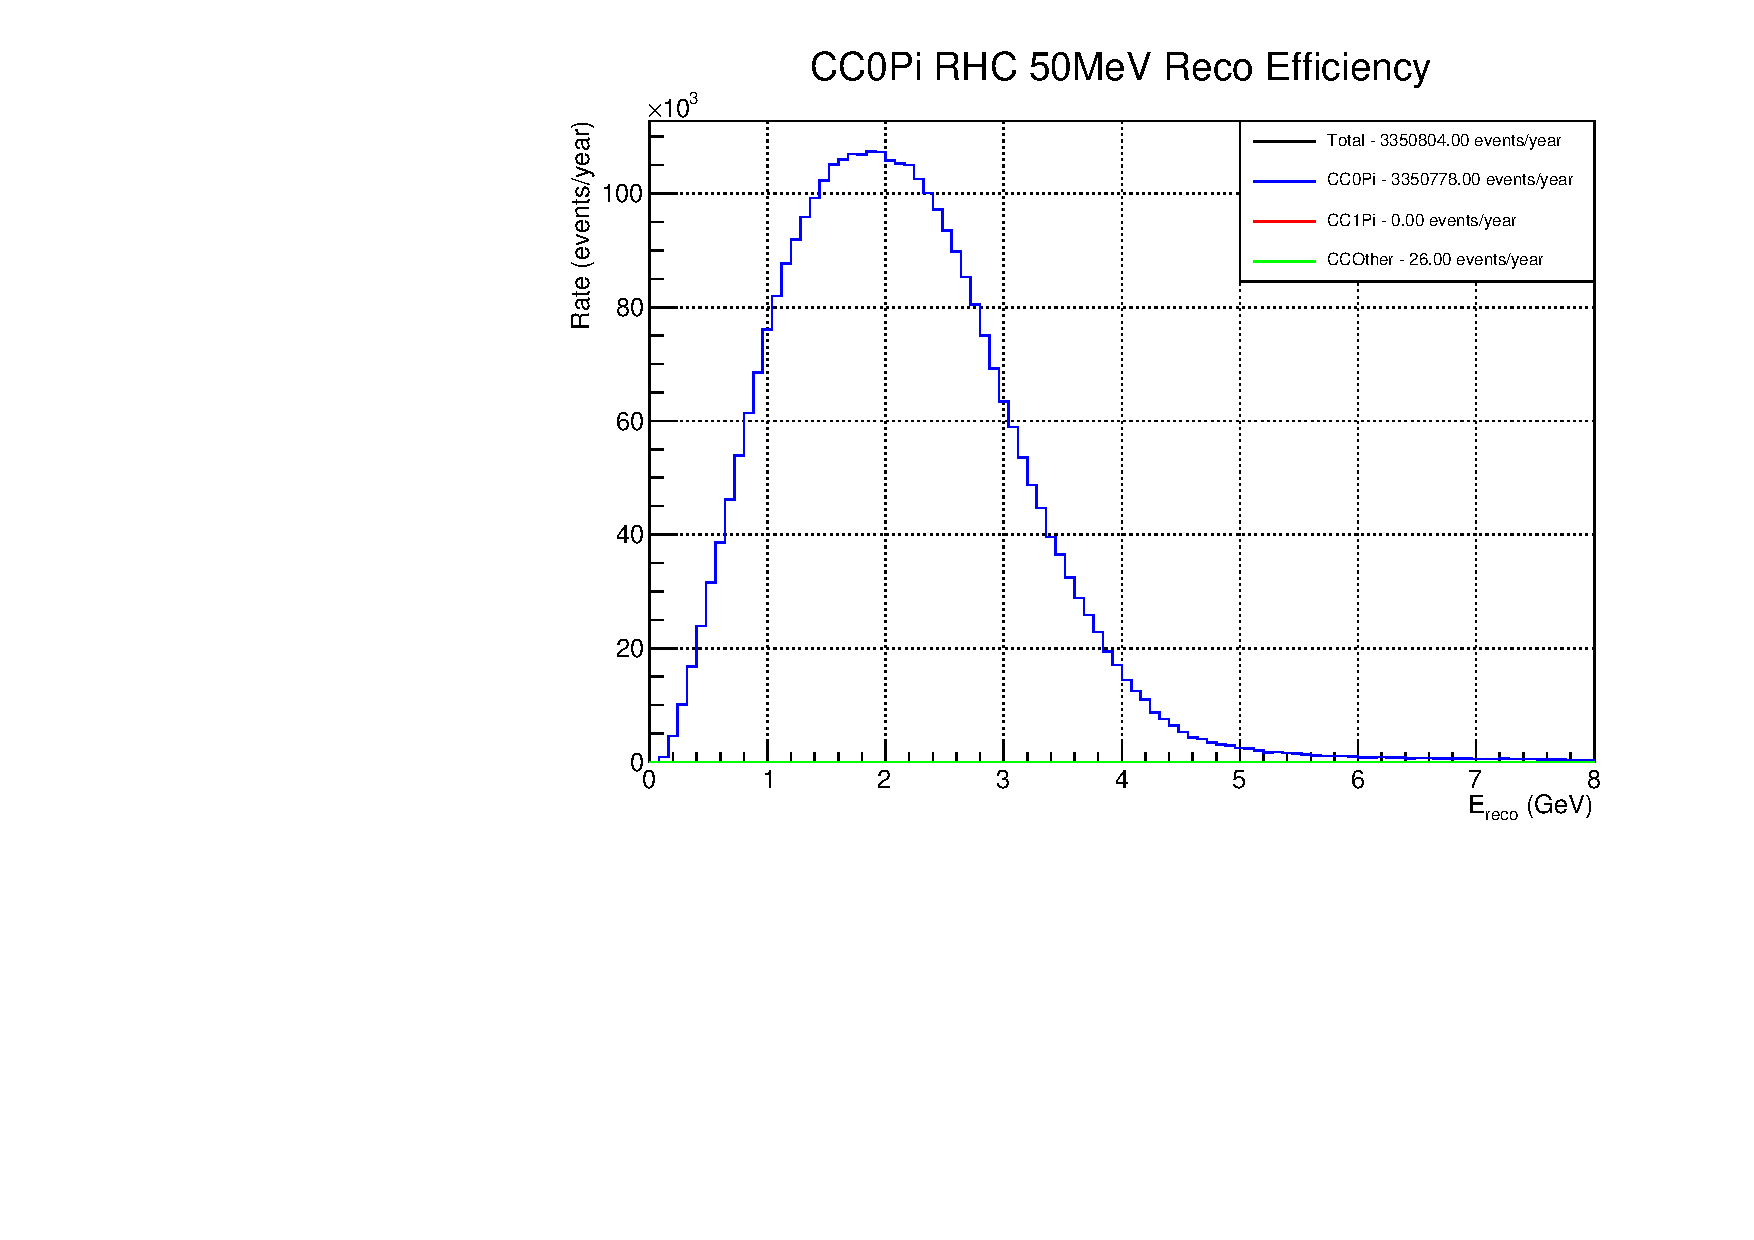
\includegraphics[width=0.245\textwidth]{plots/efficiency/CC0Pi_RHC_50MeV.pdf}

\end{center}

\subsubsection{CC1Pi}

\begin{center}

\includegraphics[width=0.245\textwidth]{plots/efficiency/CC1Pi_RHC_No_Threshold.pdf}
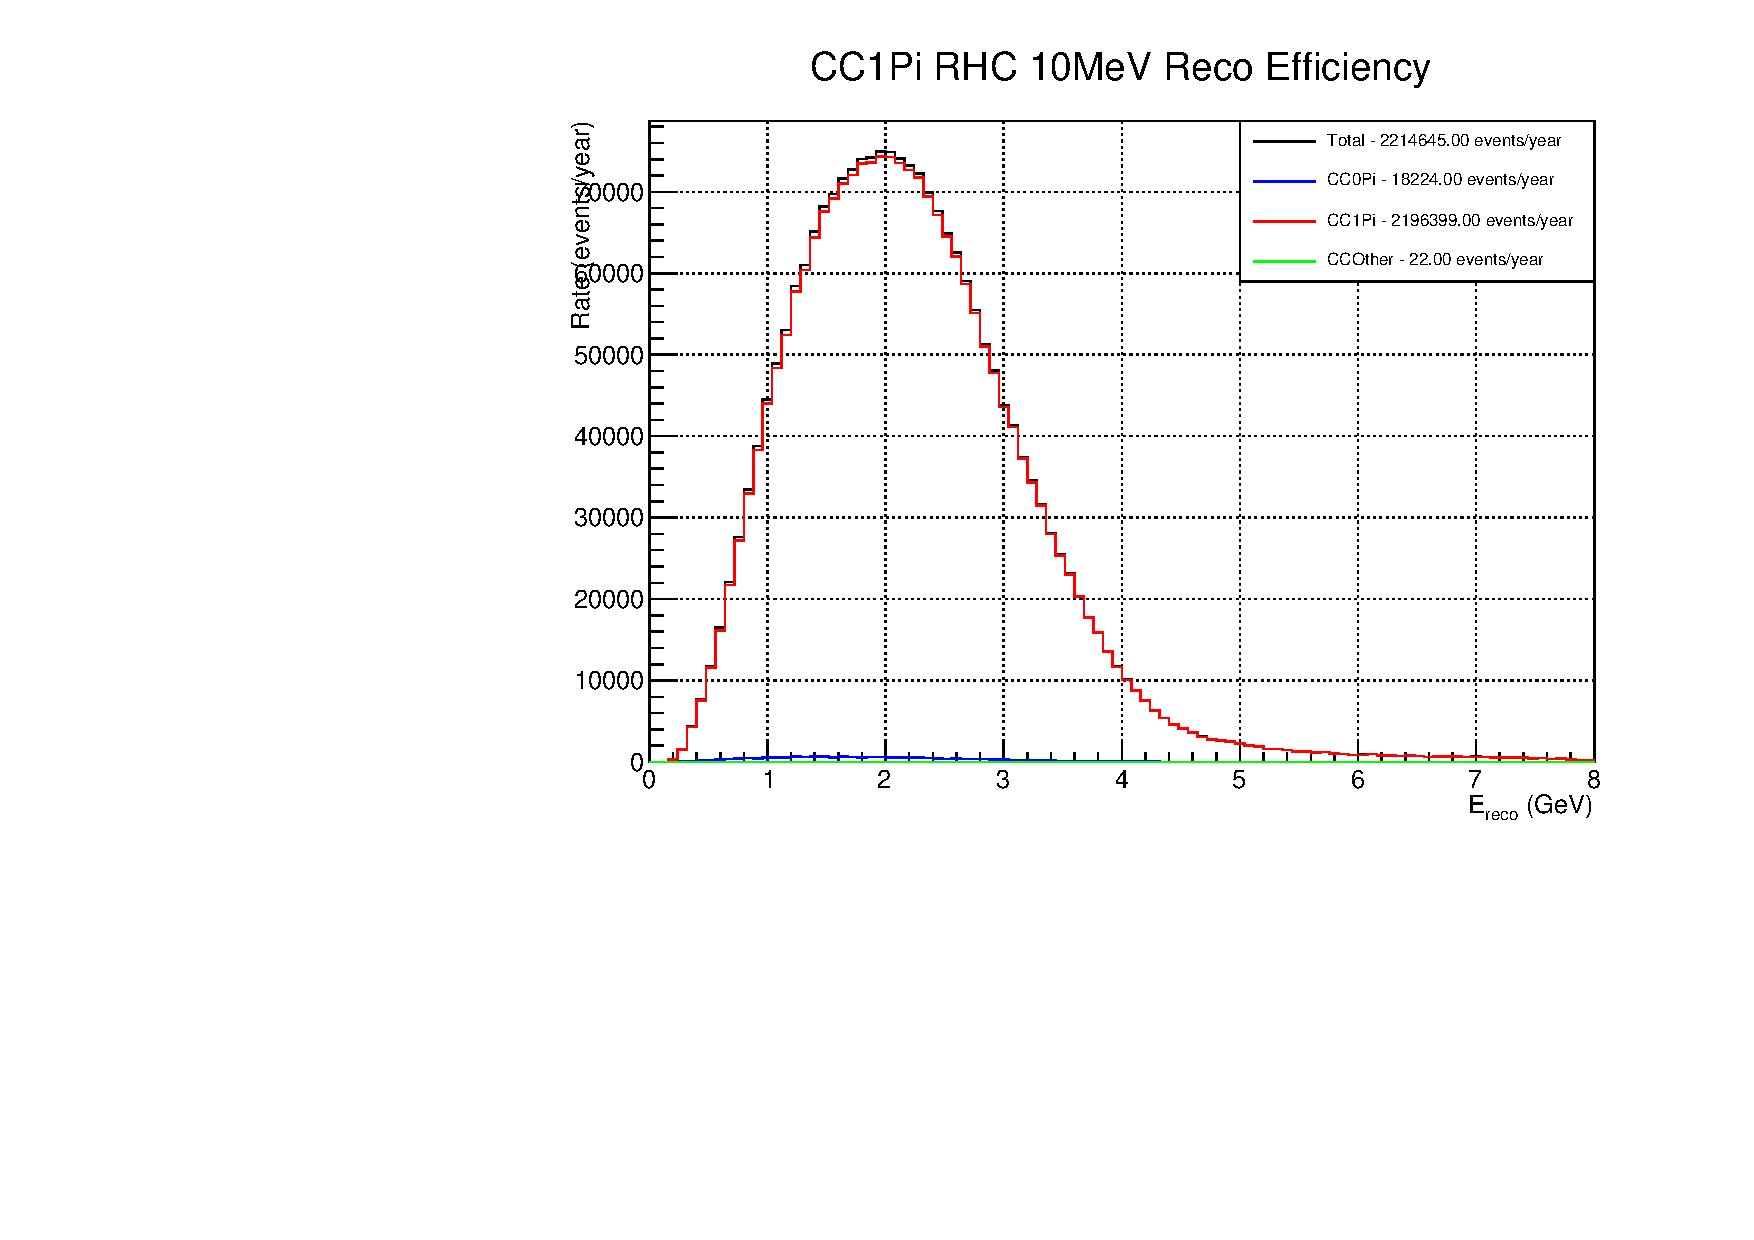
\includegraphics[width=0.245\textwidth]{plots/efficiency/CC1Pi_RHC_10MeV.pdf} 
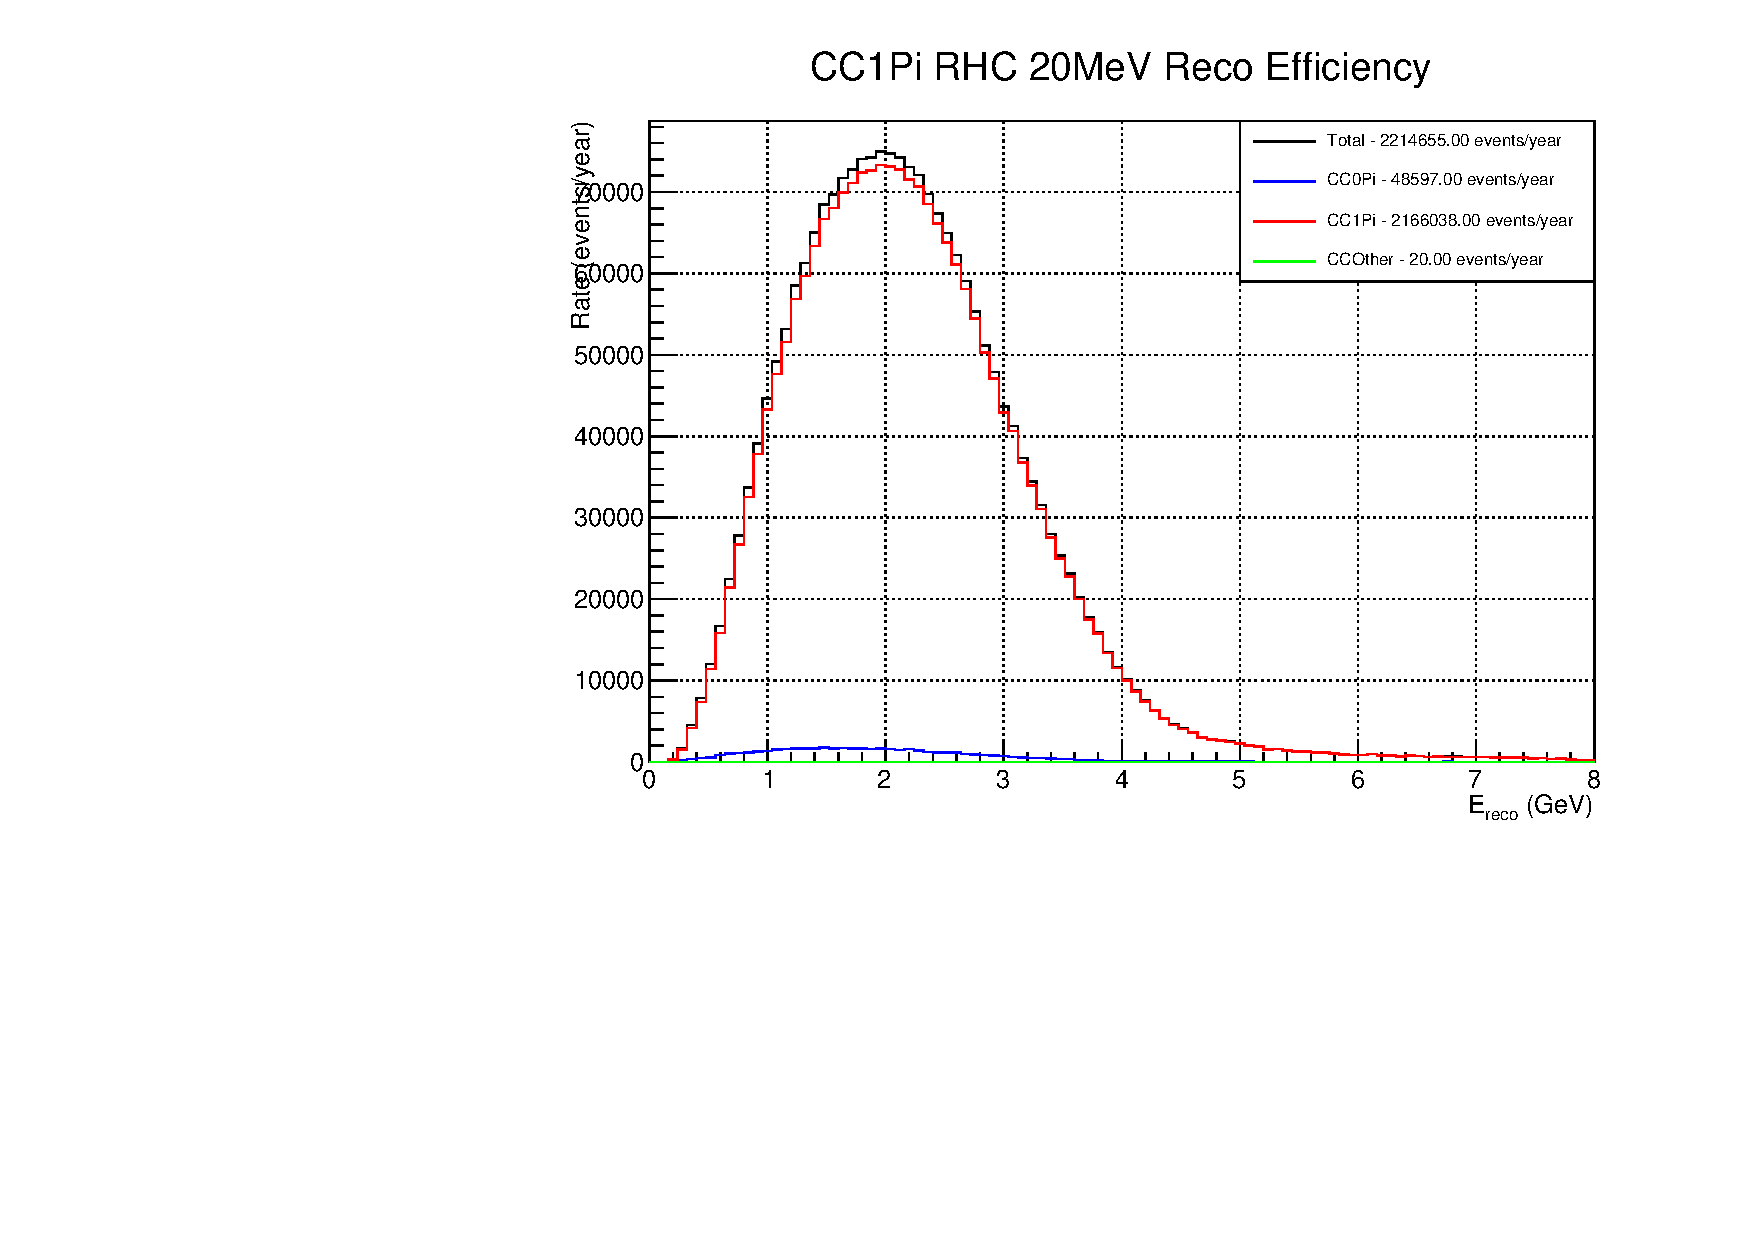
\includegraphics[width=0.245\textwidth]{plots/efficiency/CC1Pi_RHC_20MeV.pdf}
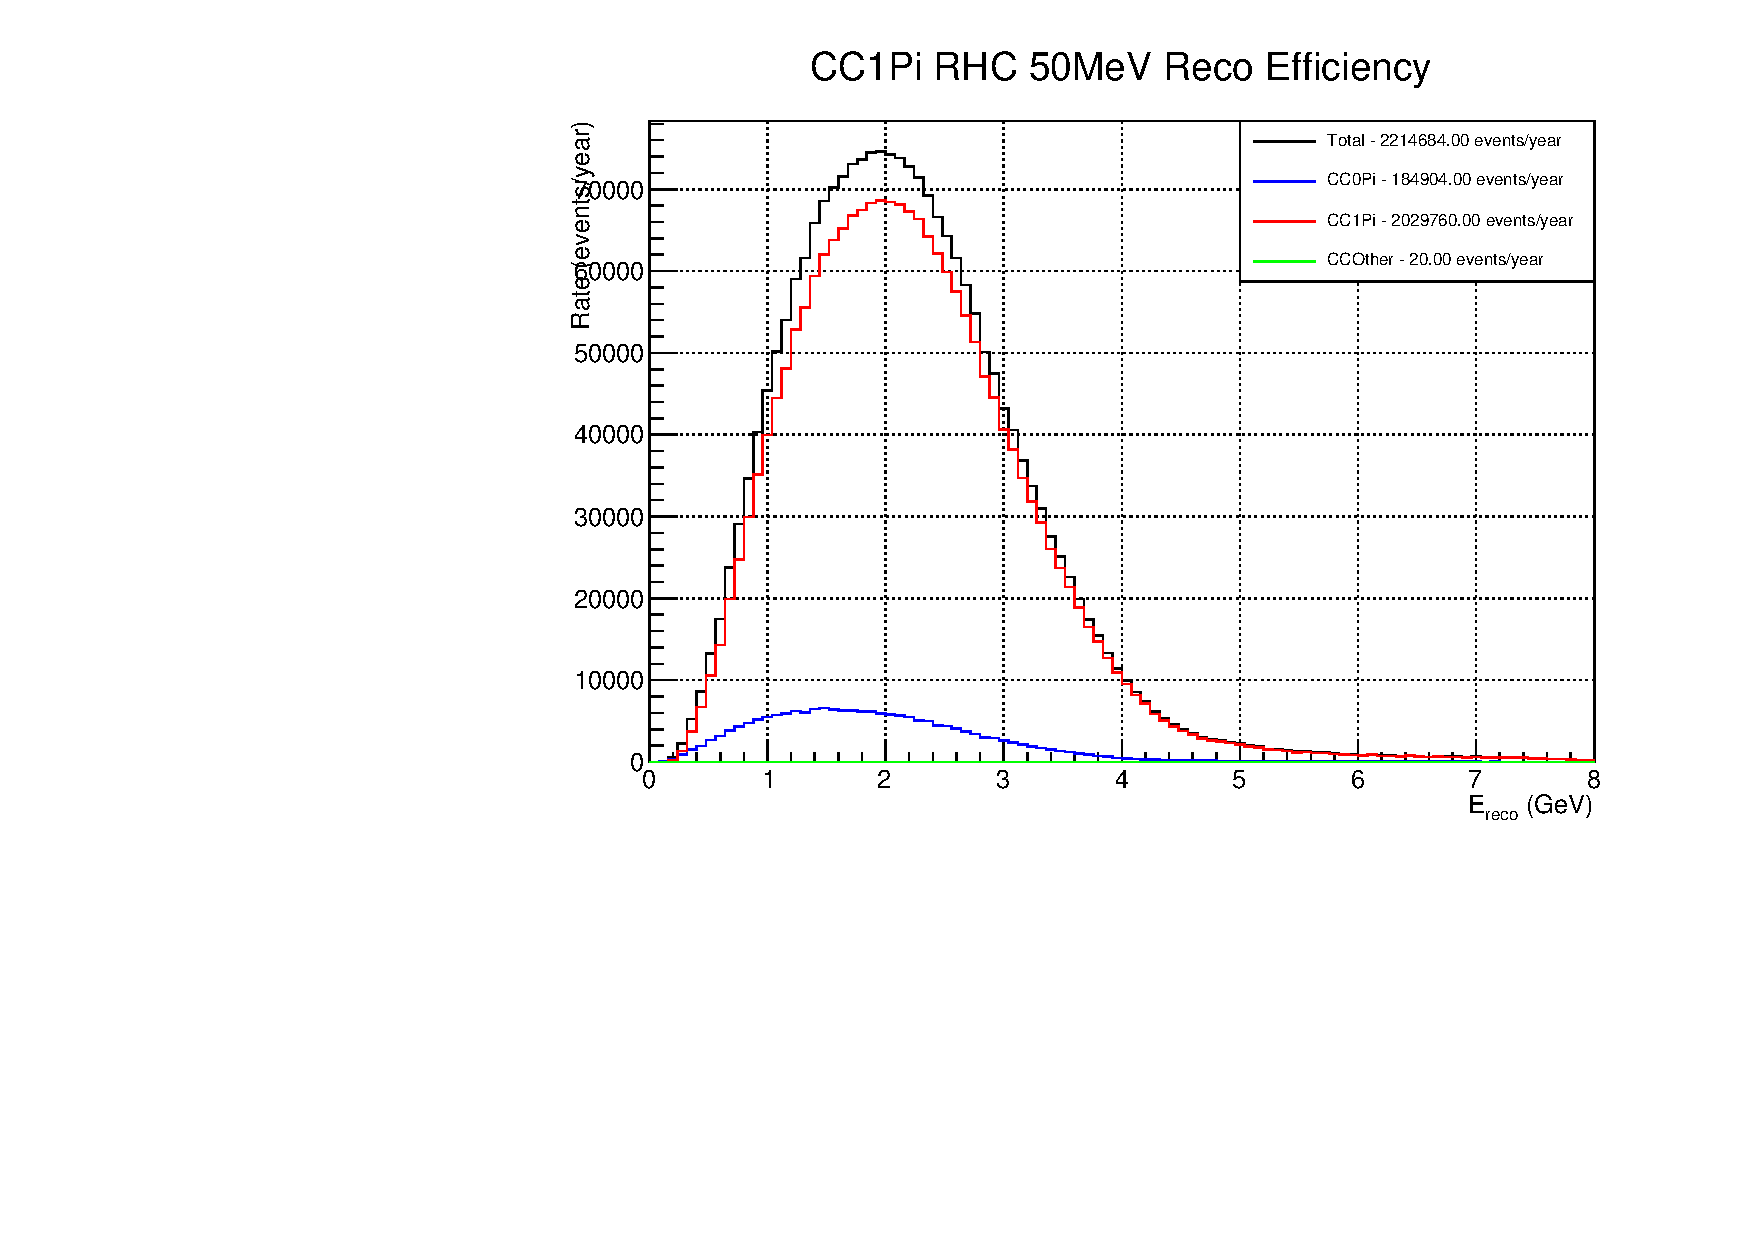
\includegraphics[width=0.245\textwidth]{plots/efficiency/CC1Pi_RHC_50MeV.pdf}

\end{center}

\subsubsection{CCOther}

\begin{center}

\includegraphics[width=0.245\textwidth]{plots/efficiency/CCOther_RHC_No_Threshold.pdf}
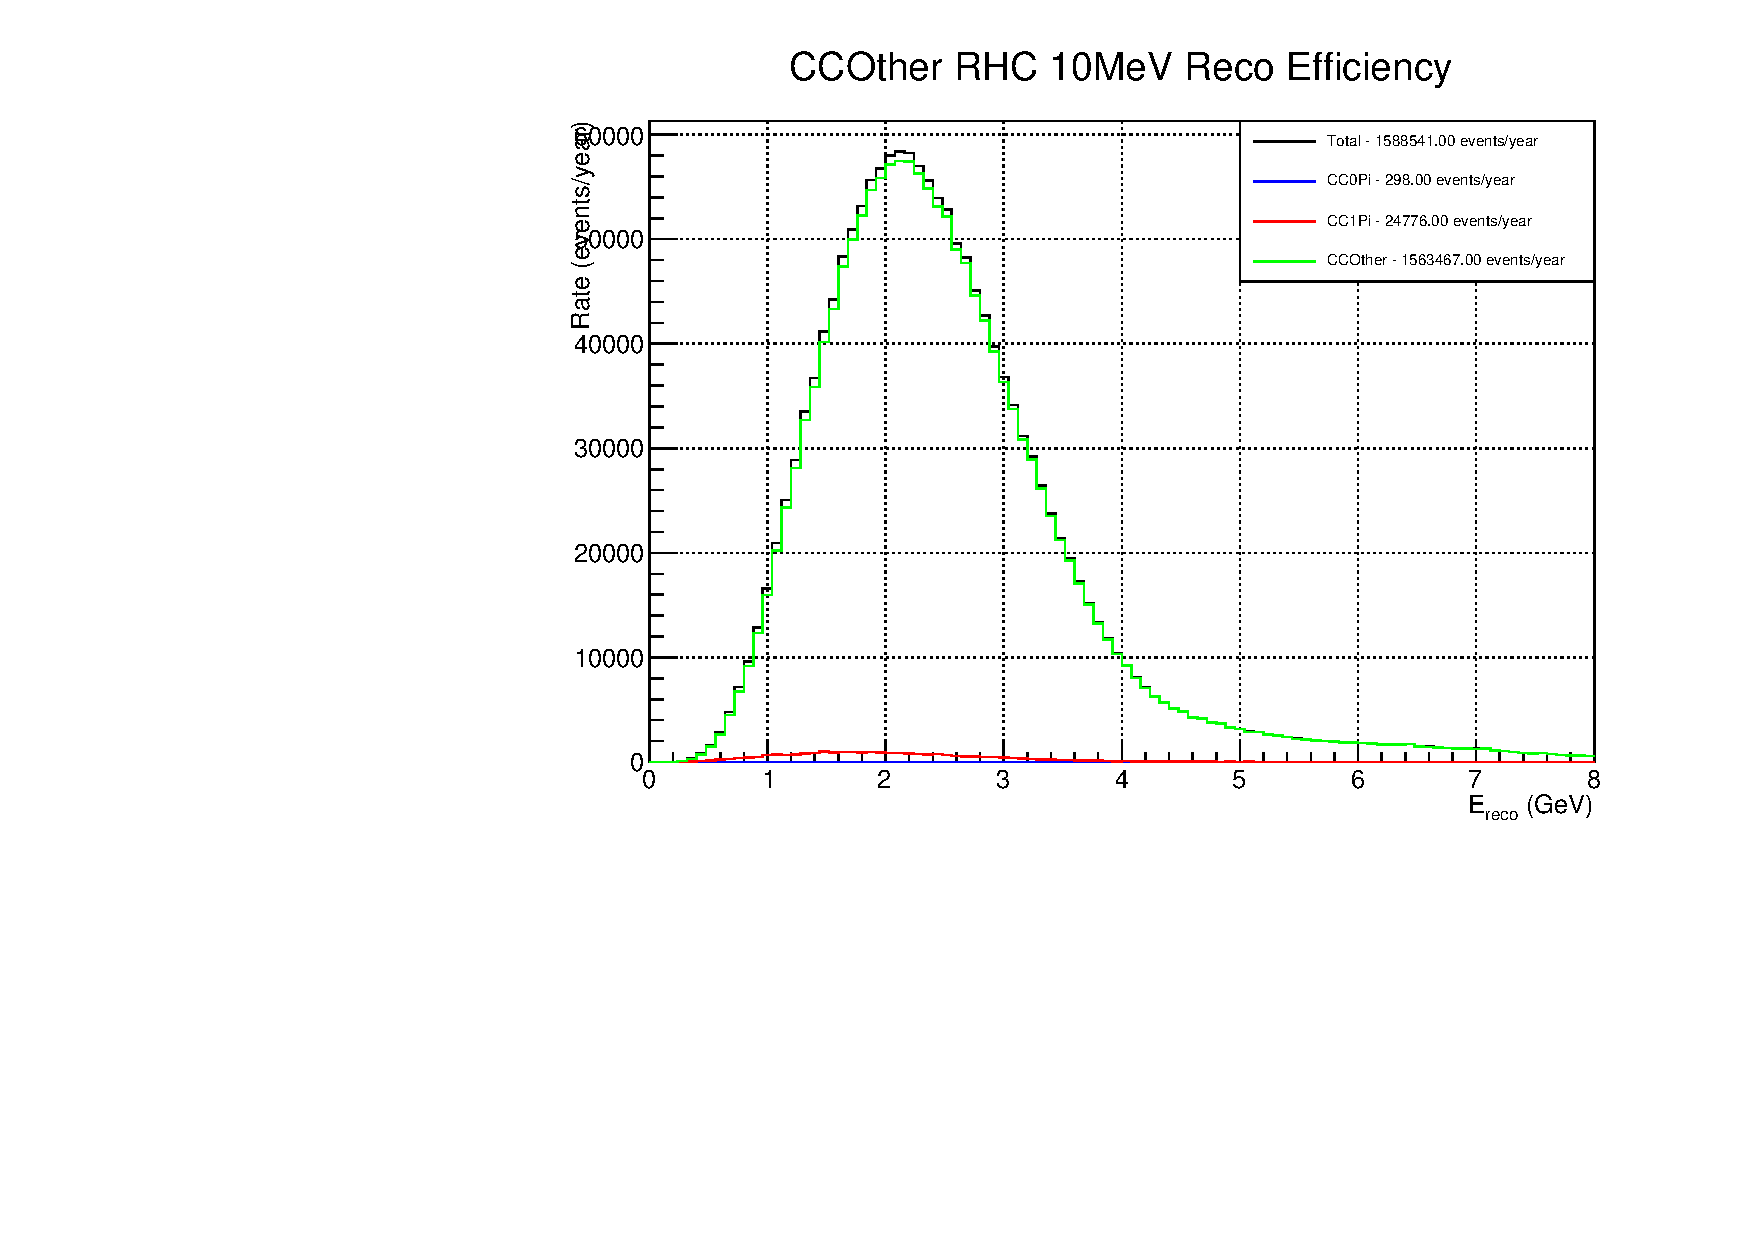
\includegraphics[width=0.245\textwidth]{plots/efficiency/CCOther_RHC_10MeV.pdf} 
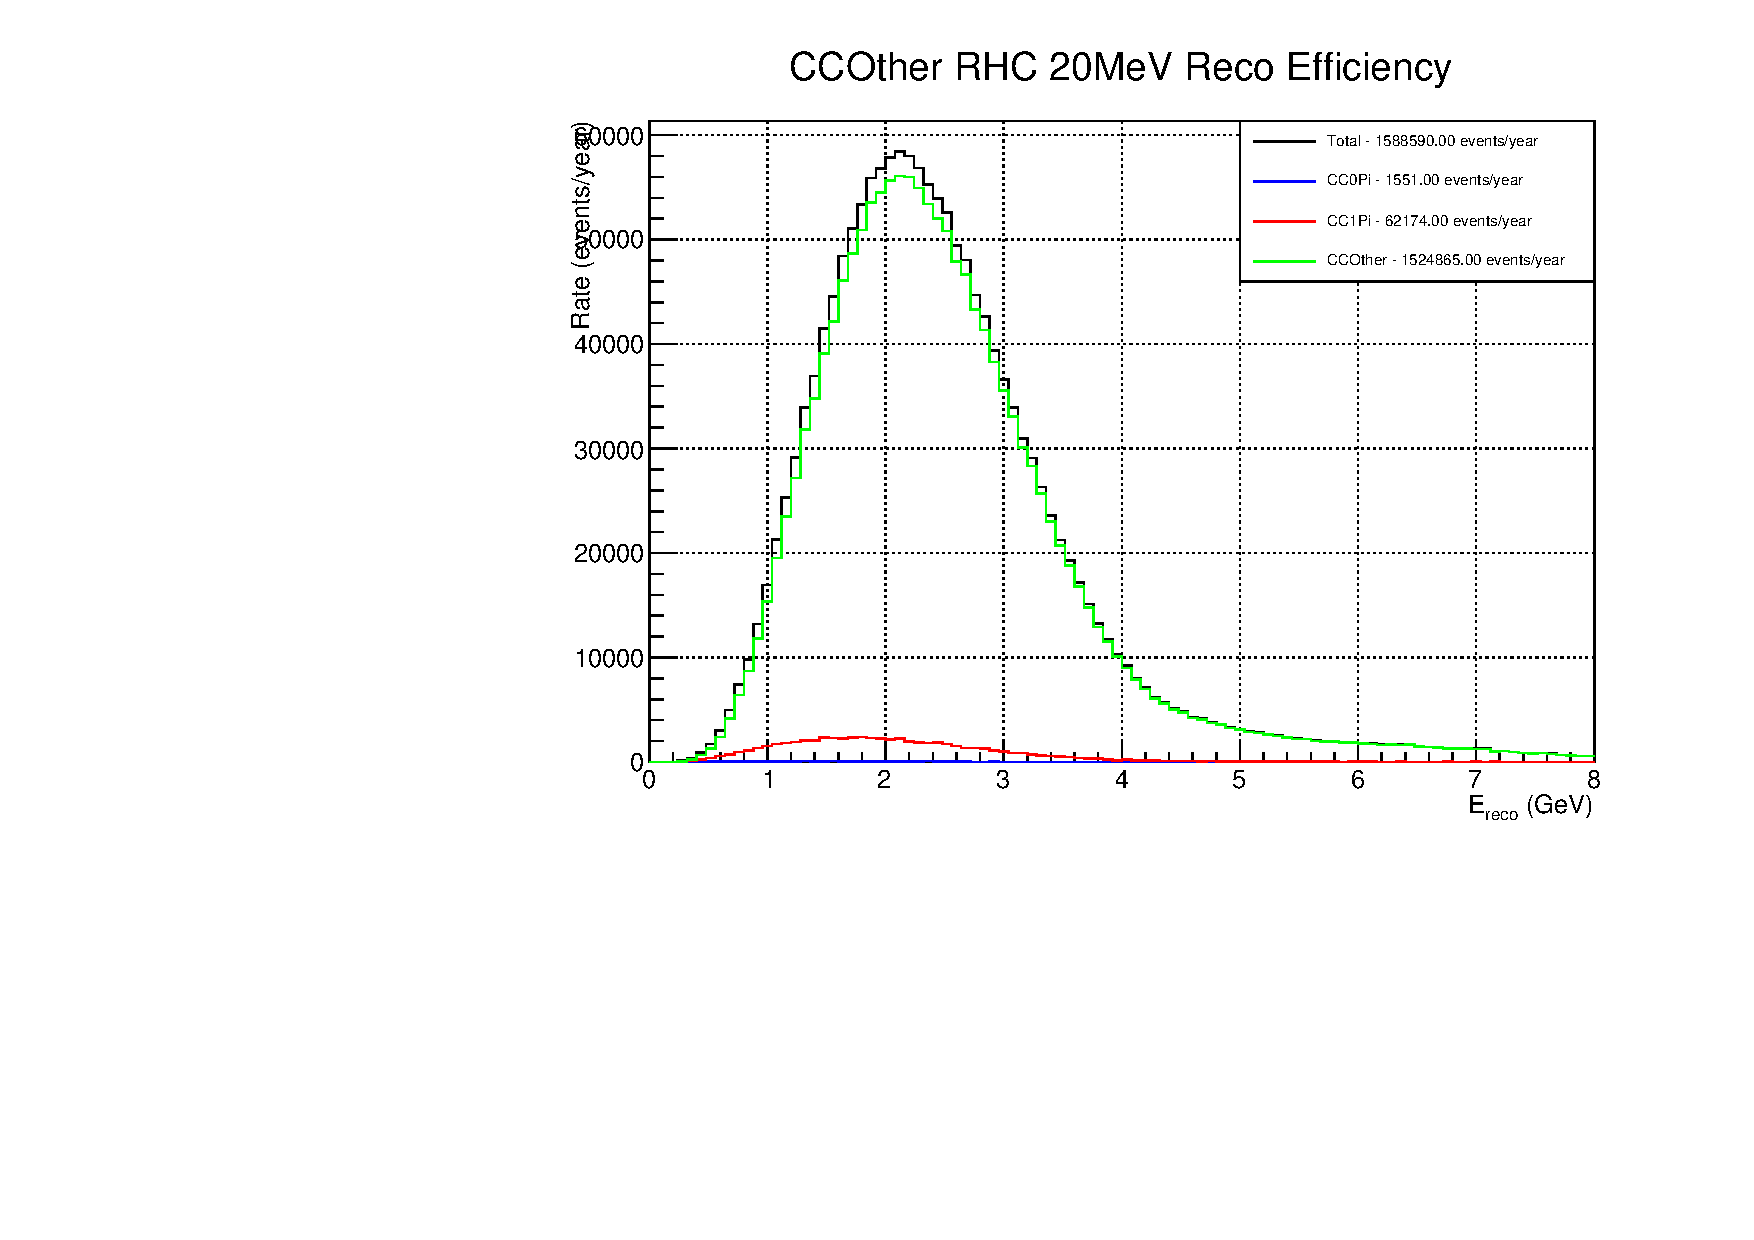
\includegraphics[width=0.245\textwidth]{plots/efficiency/CCOther_RHC_20MeV.pdf}
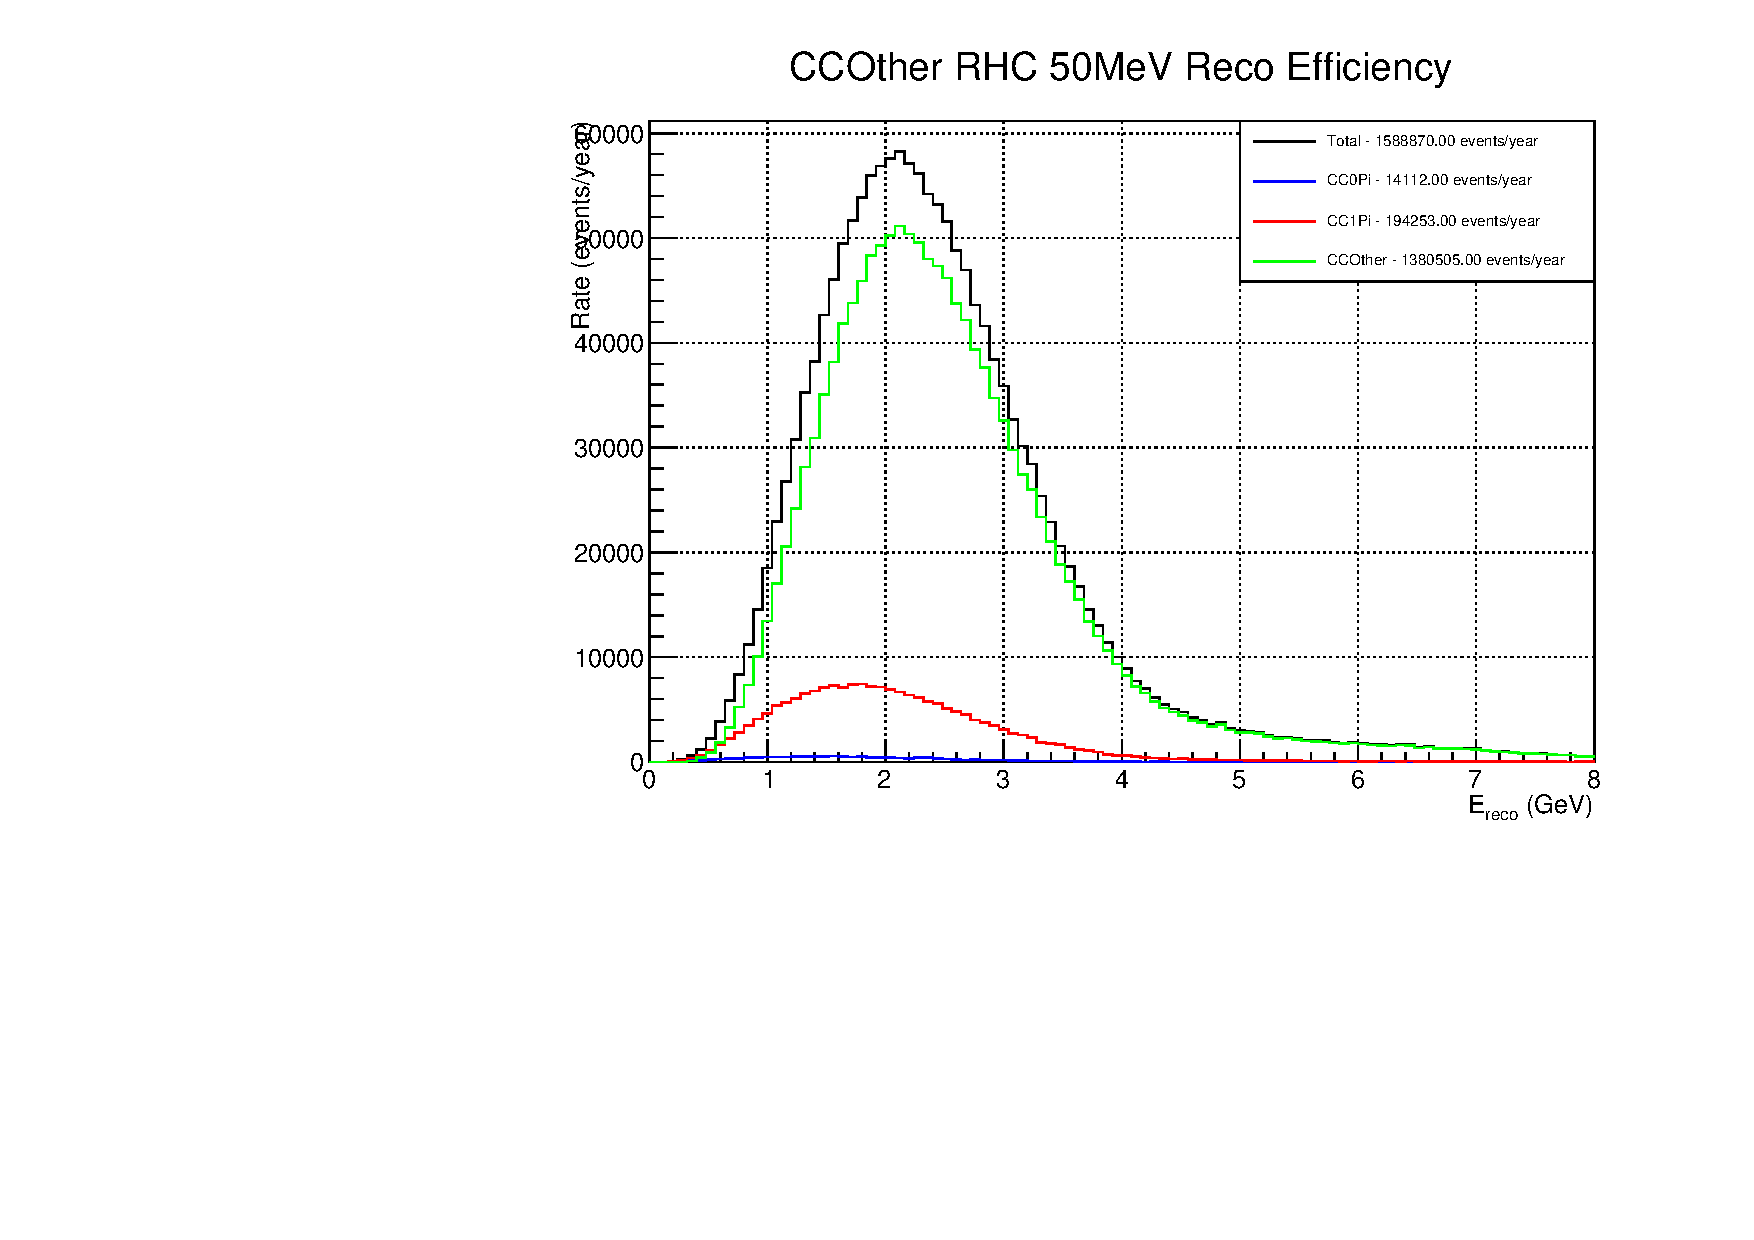
\includegraphics[width=0.245\textwidth]{plots/efficiency/CCOther_RHC_50MeV.pdf}

\end{center}


\section{Purity}

Purity is defined here as the migration to a given reconstructed topology from all true topologies.  The following plots are separated in terms of the reconstructed topology and show the true topology of the events that reconstruct to that topology.

\subsection{FHC}

\subsubsection{CC0Pi}

Events of any true topology can reconstruct to CC0Pi.

\begin{center}

\includegraphics[width=0.245\textwidth]{plots/purity/CC0Pi_FHC_No_Threshold.pdf}
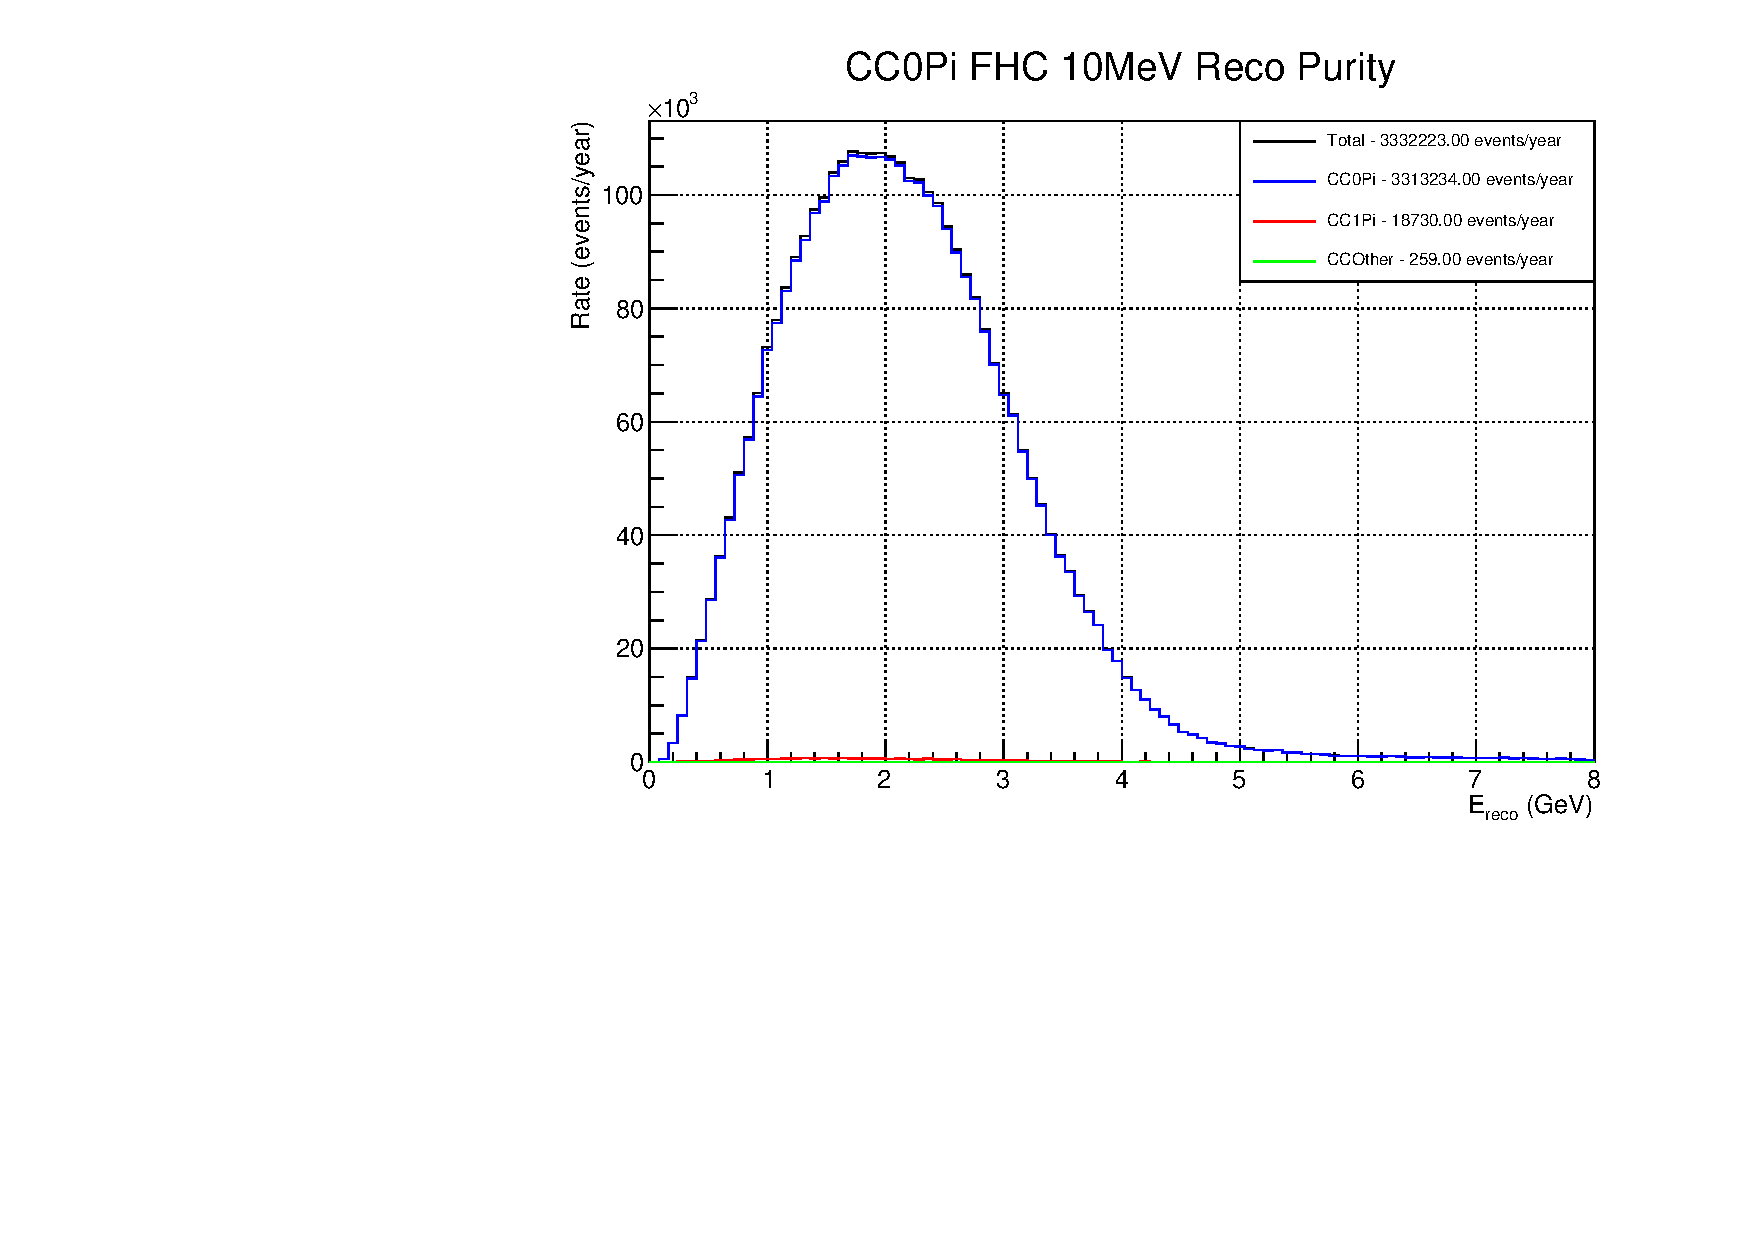
\includegraphics[width=0.245\textwidth]{plots/purity/CC0Pi_FHC_10MeV.pdf} 
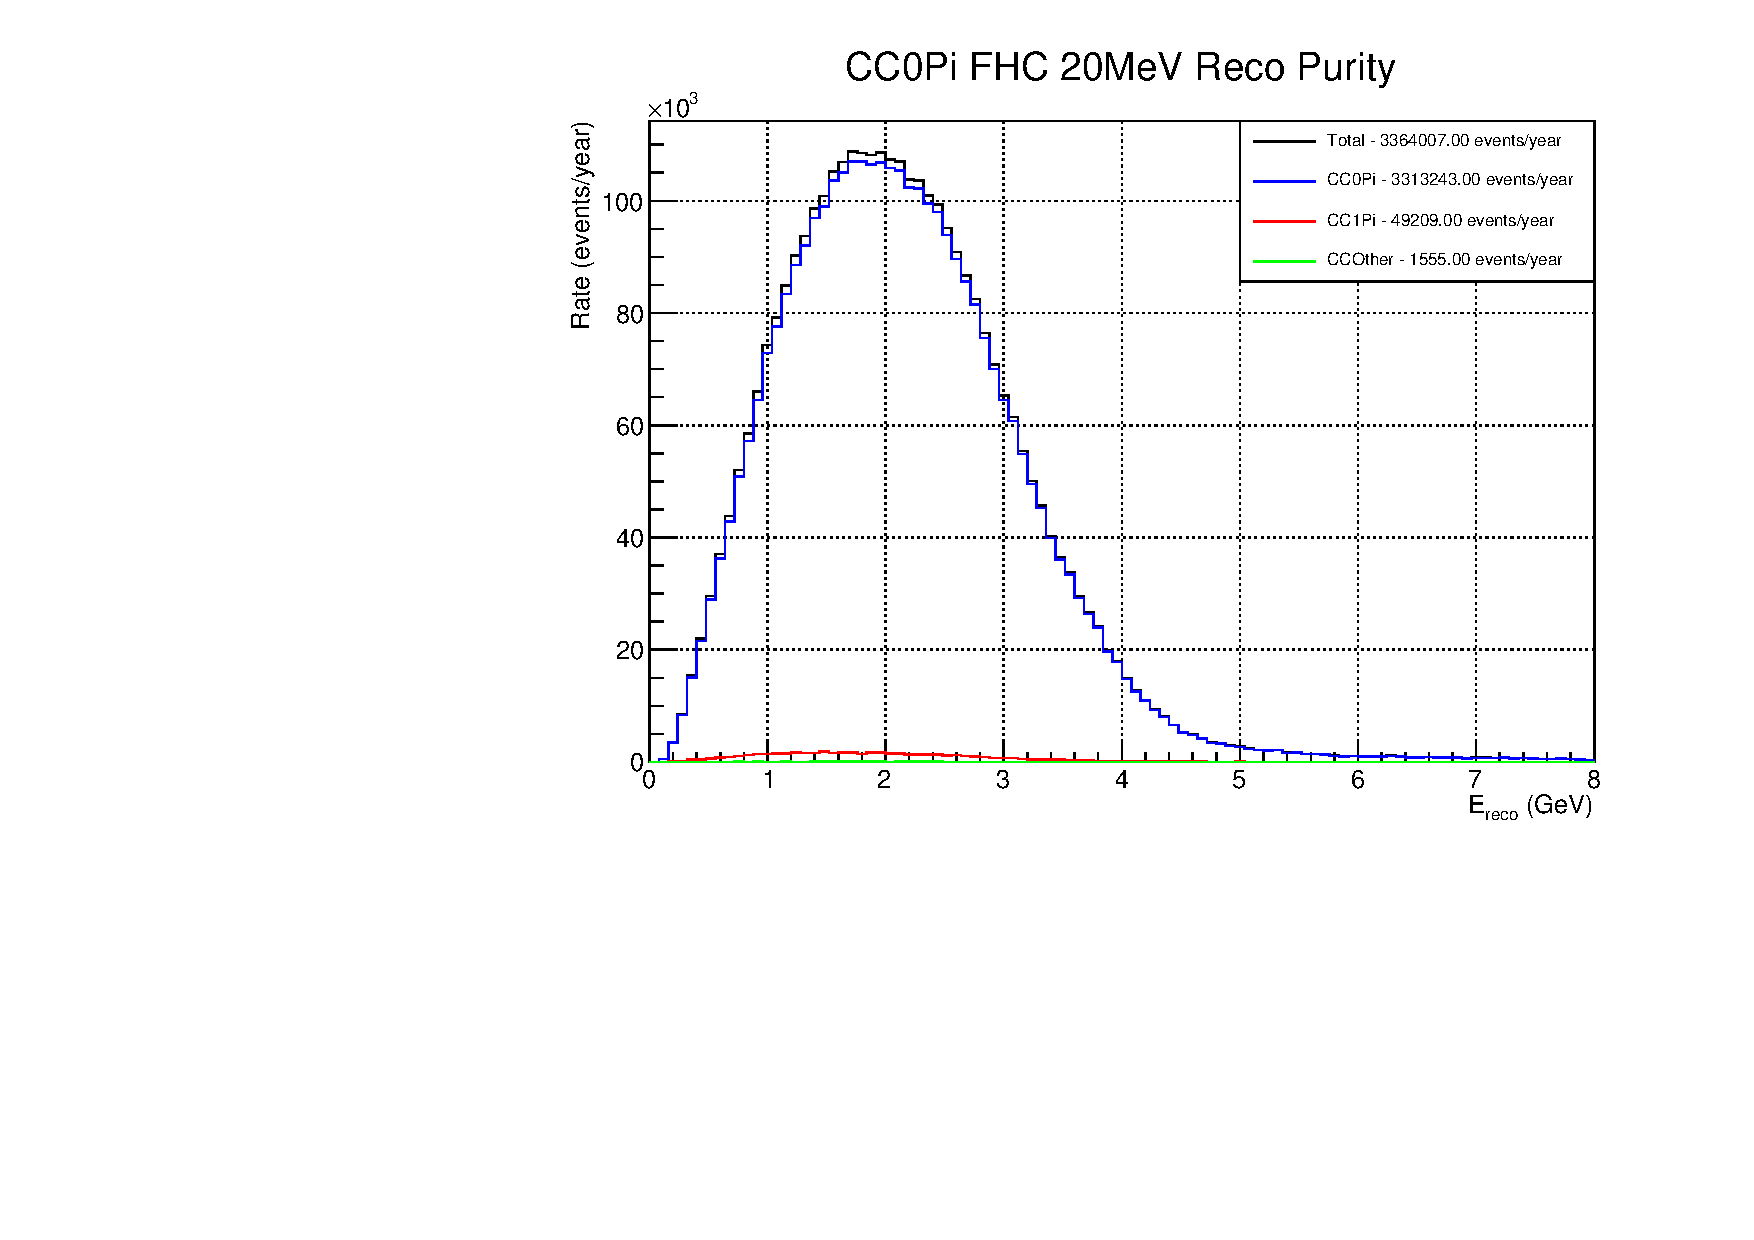
\includegraphics[width=0.245\textwidth]{plots/purity/CC0Pi_FHC_20MeV.pdf}
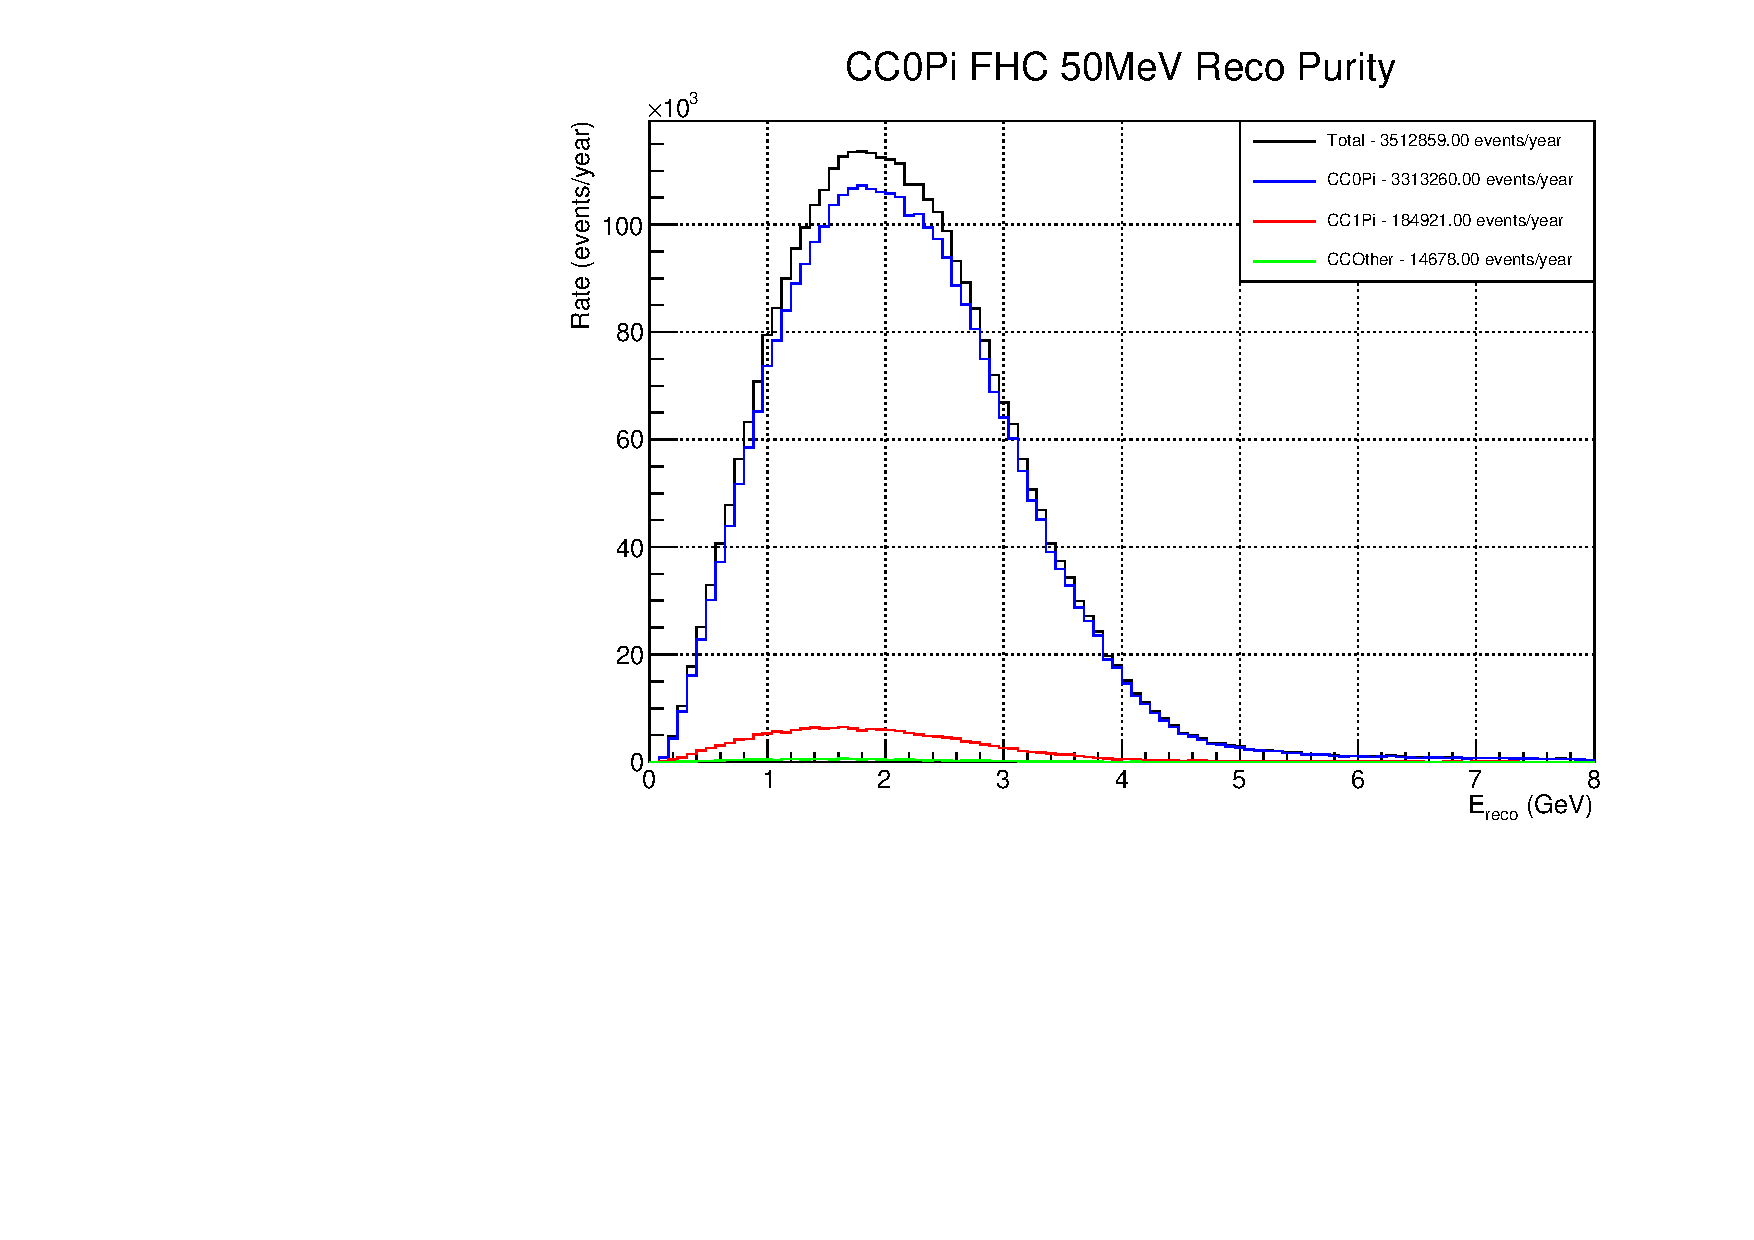
\includegraphics[width=0.245\textwidth]{plots/purity/CC0Pi_FHC_50MeV.pdf}

\end{center}

\subsubsection{CC1Pi}

Only CCOther events can reconstruct to CC1Pi

\begin{center}

\includegraphics[width=0.245\textwidth]{plots/purity/CC1Pi_FHC_No_Threshold.pdf}
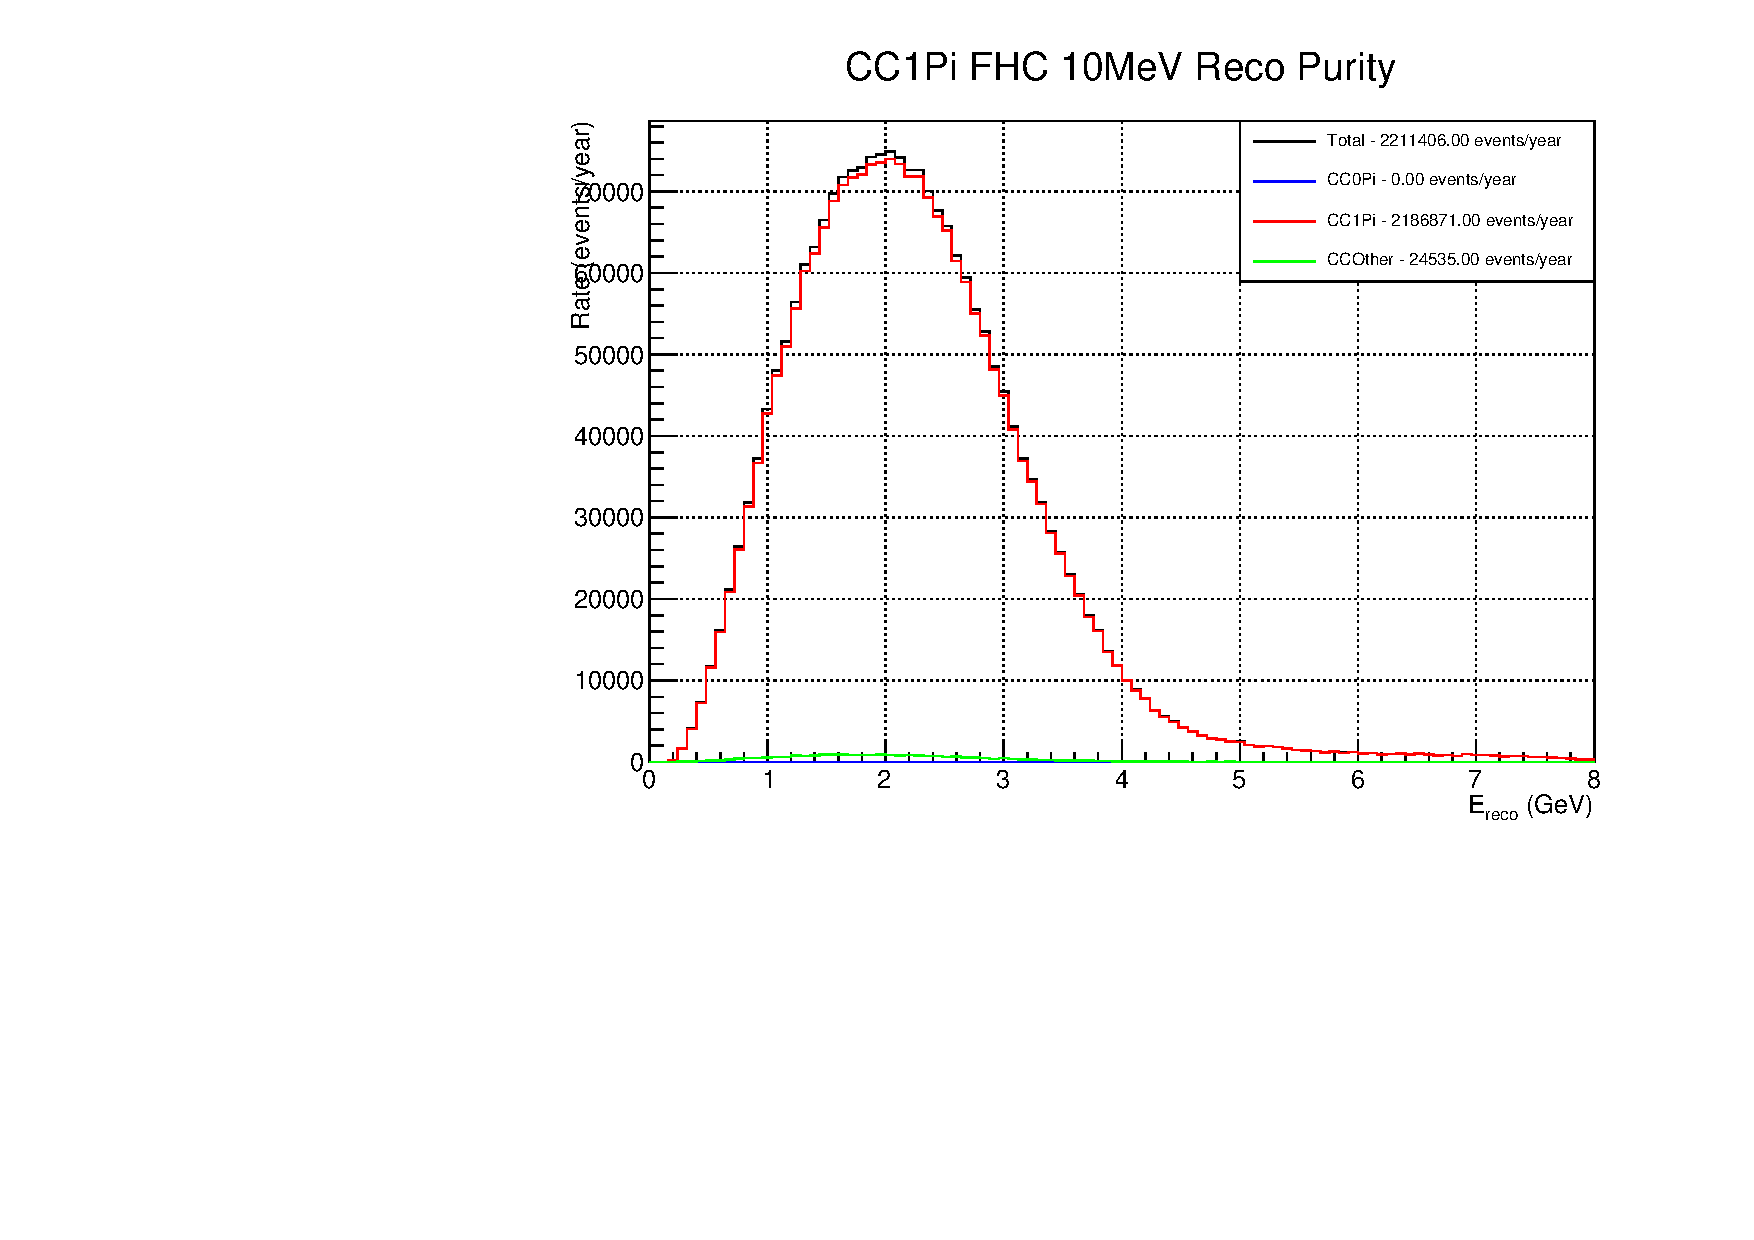
\includegraphics[width=0.245\textwidth]{plots/purity/CC1Pi_FHC_10MeV.pdf} 
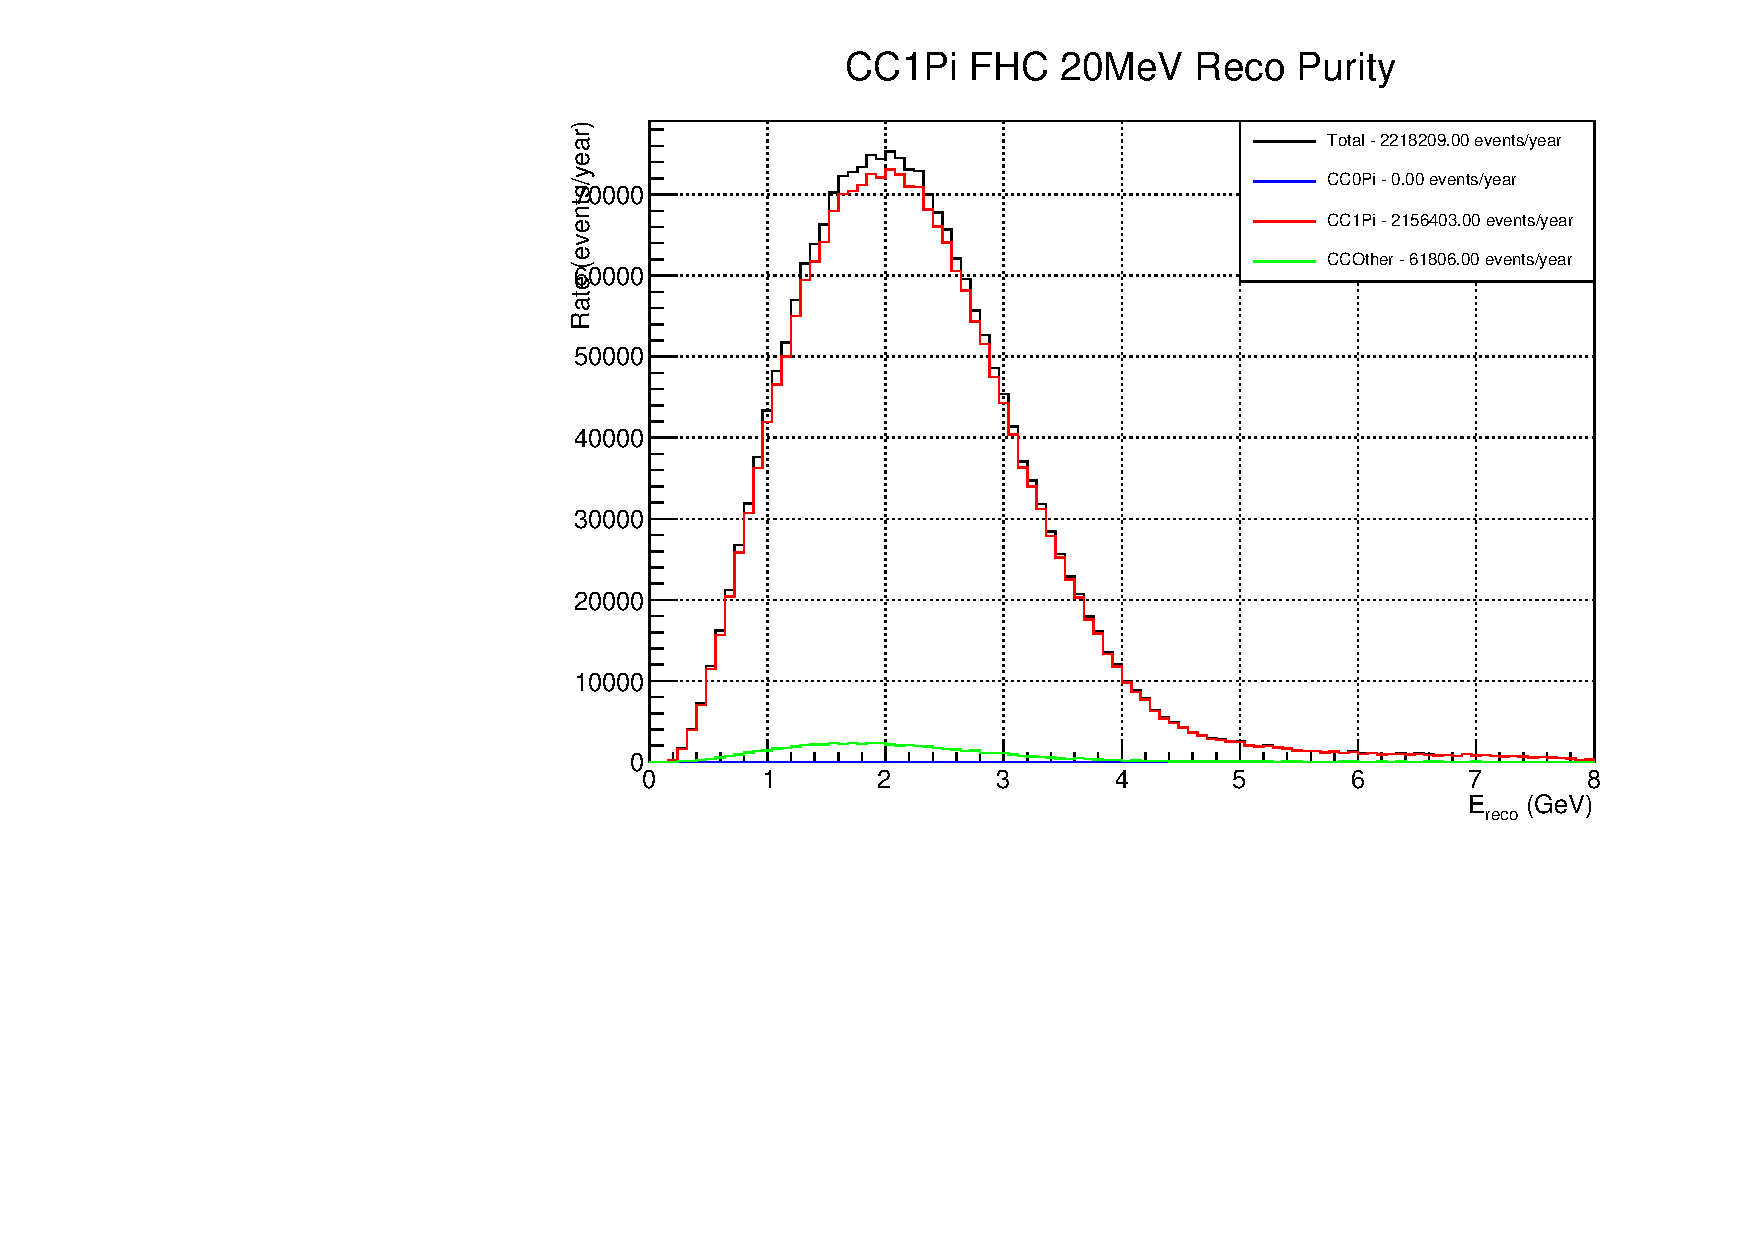
\includegraphics[width=0.245\textwidth]{plots/purity/CC1Pi_FHC_20MeV.pdf}
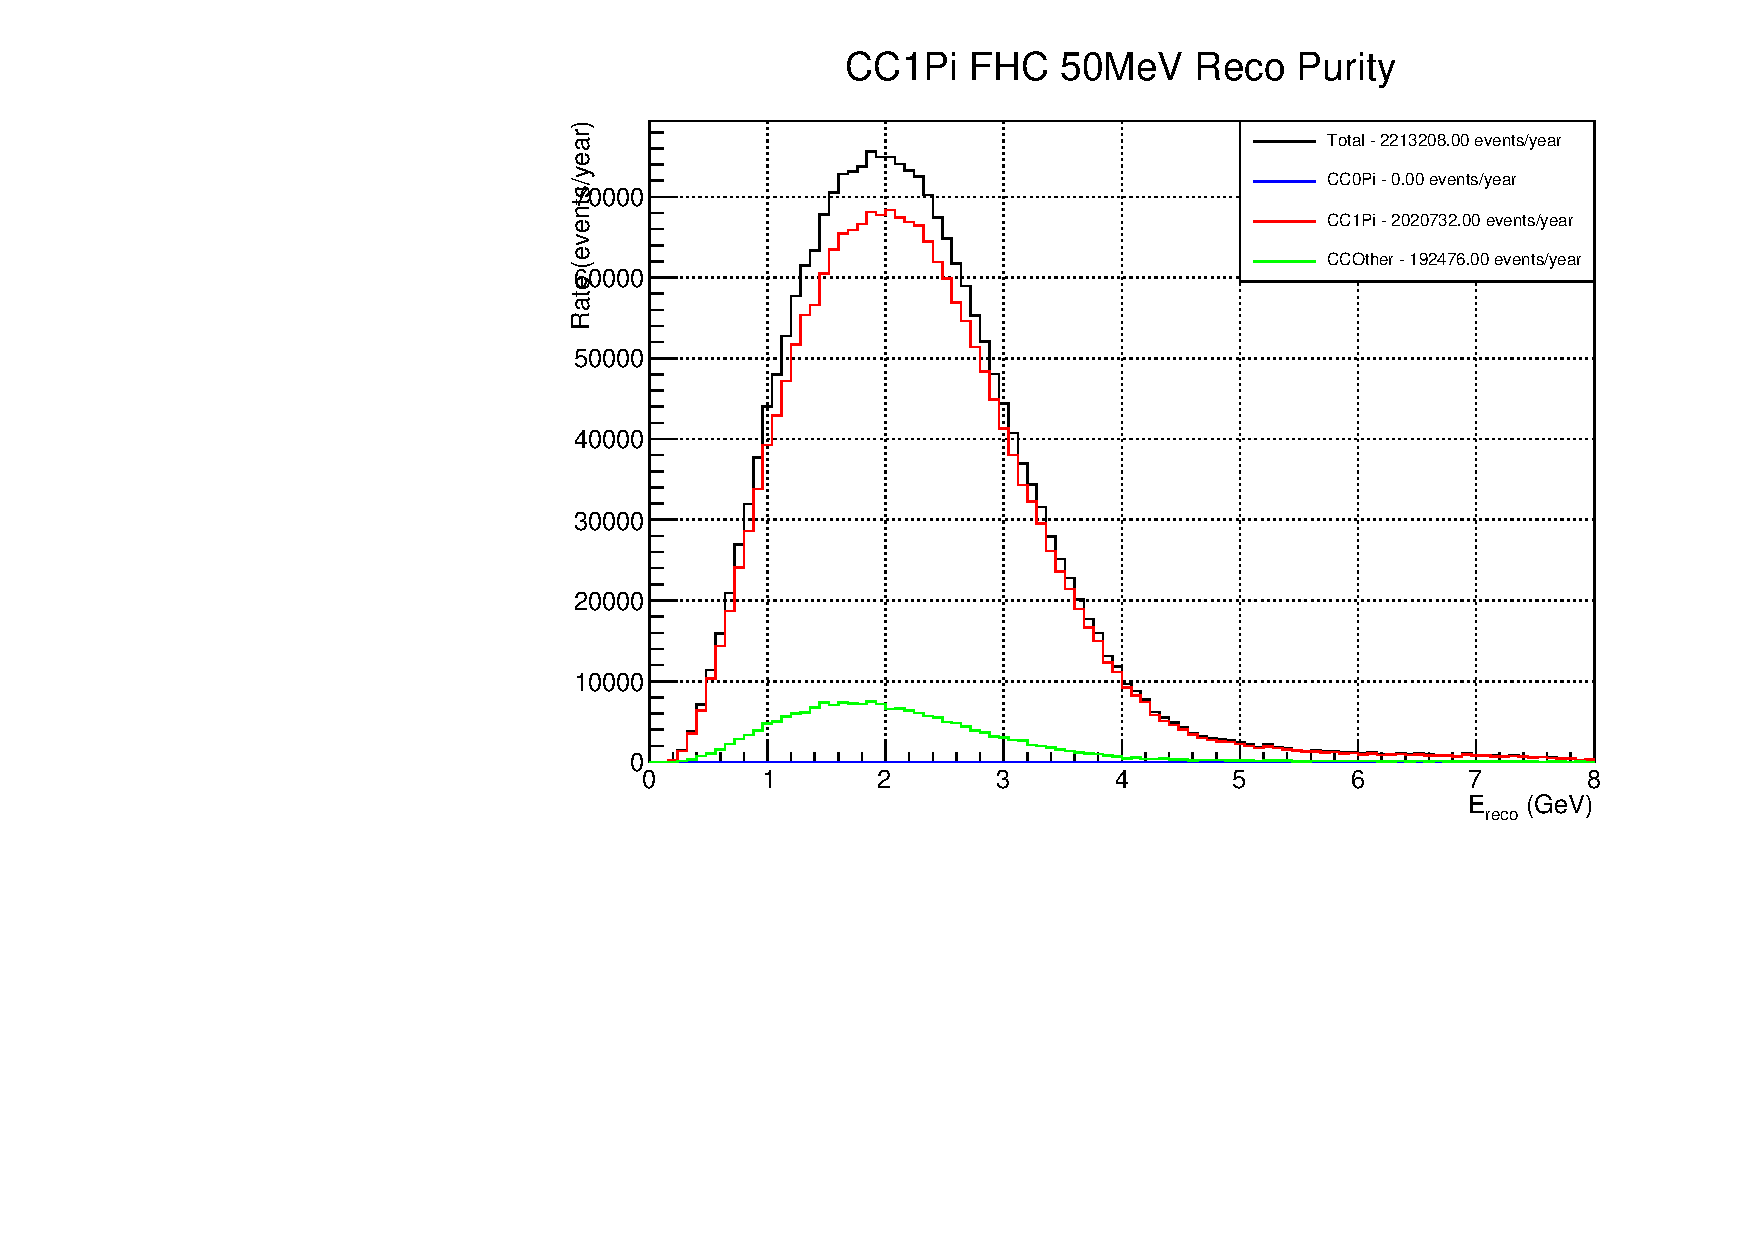
\includegraphics[width=0.245\textwidth]{plots/purity/CC1Pi_FHC_50MeV.pdf}

\end{center}

\subsubsection{CCOther}

Events reconstructed as CCOther events will always be true CCOther events.

\begin{center}

\includegraphics[width=0.245\textwidth]{plots/purity/CCOther_FHC_No_Threshold.pdf}
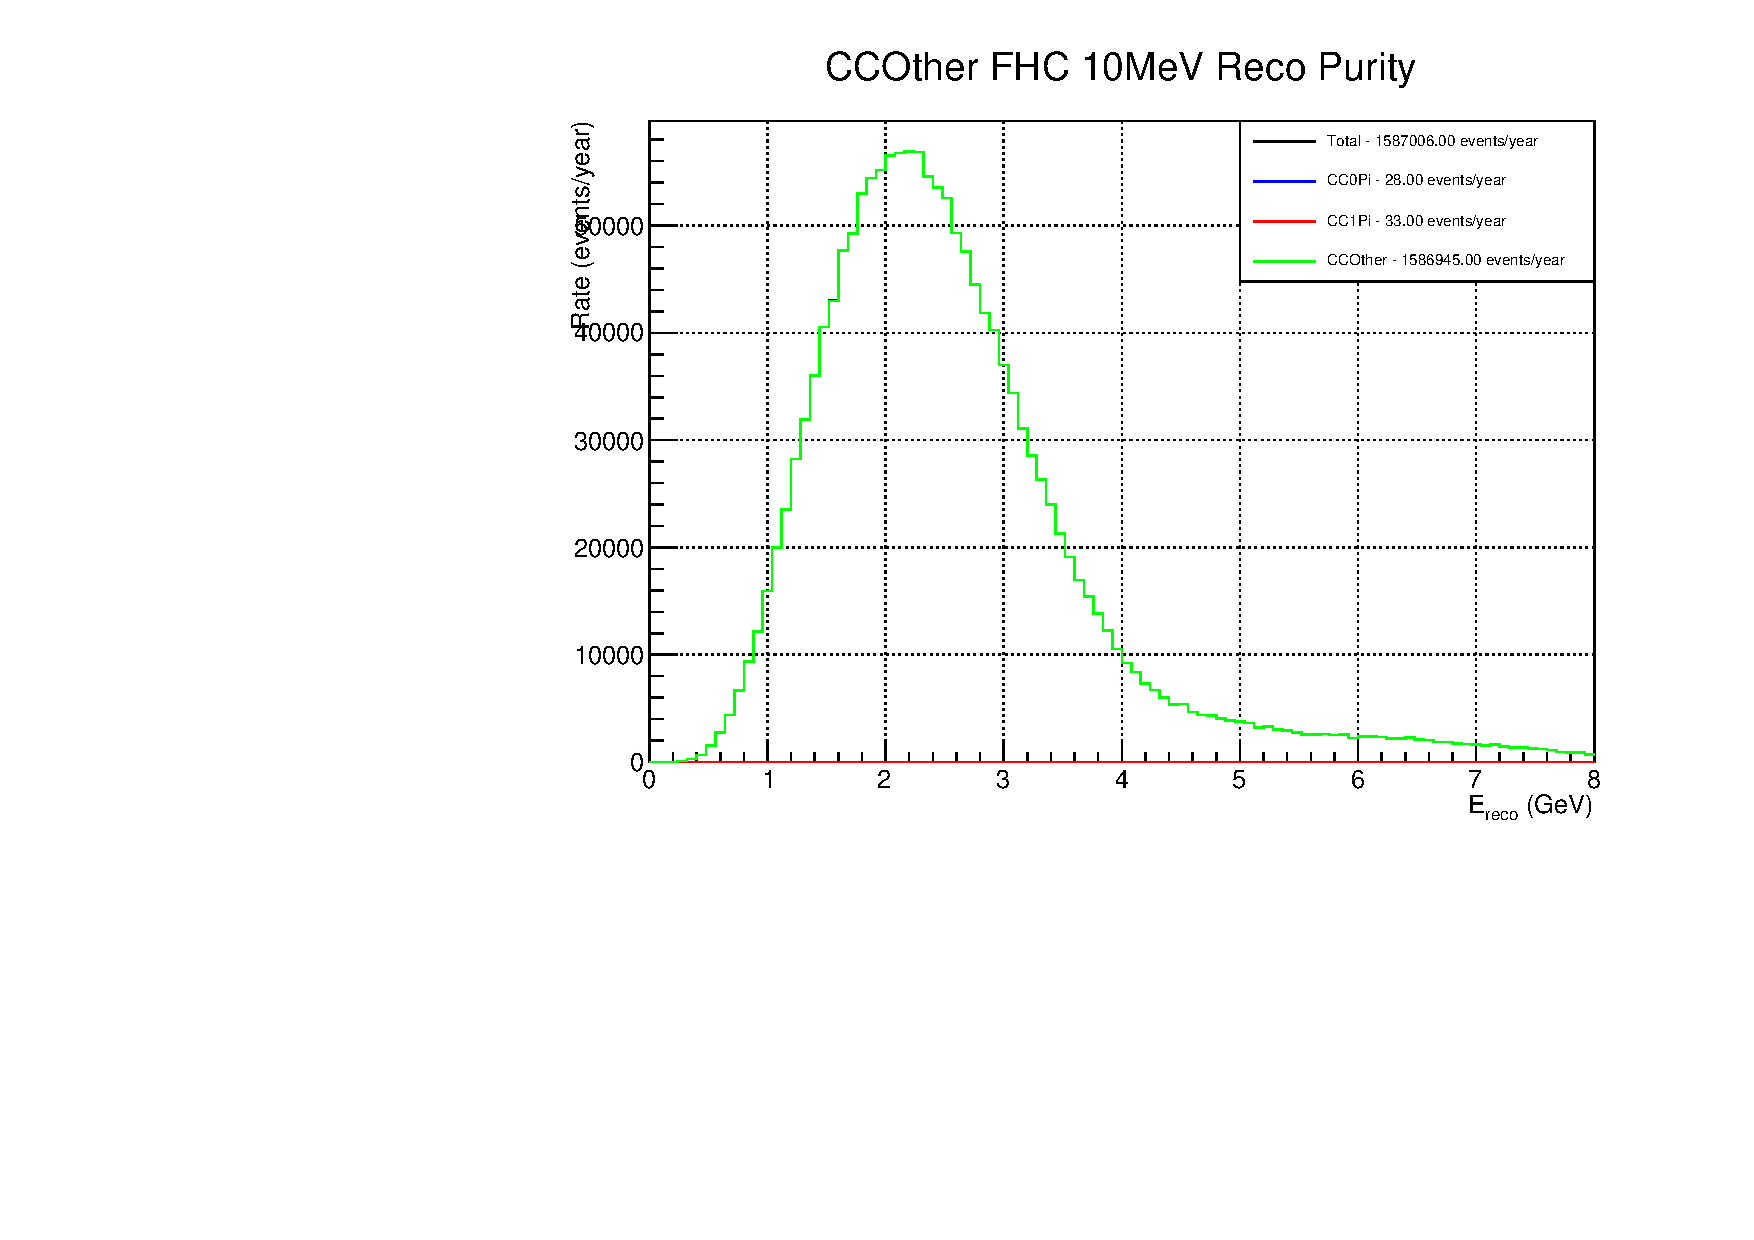
\includegraphics[width=0.245\textwidth]{plots/purity/CCOther_FHC_10MeV.pdf} 
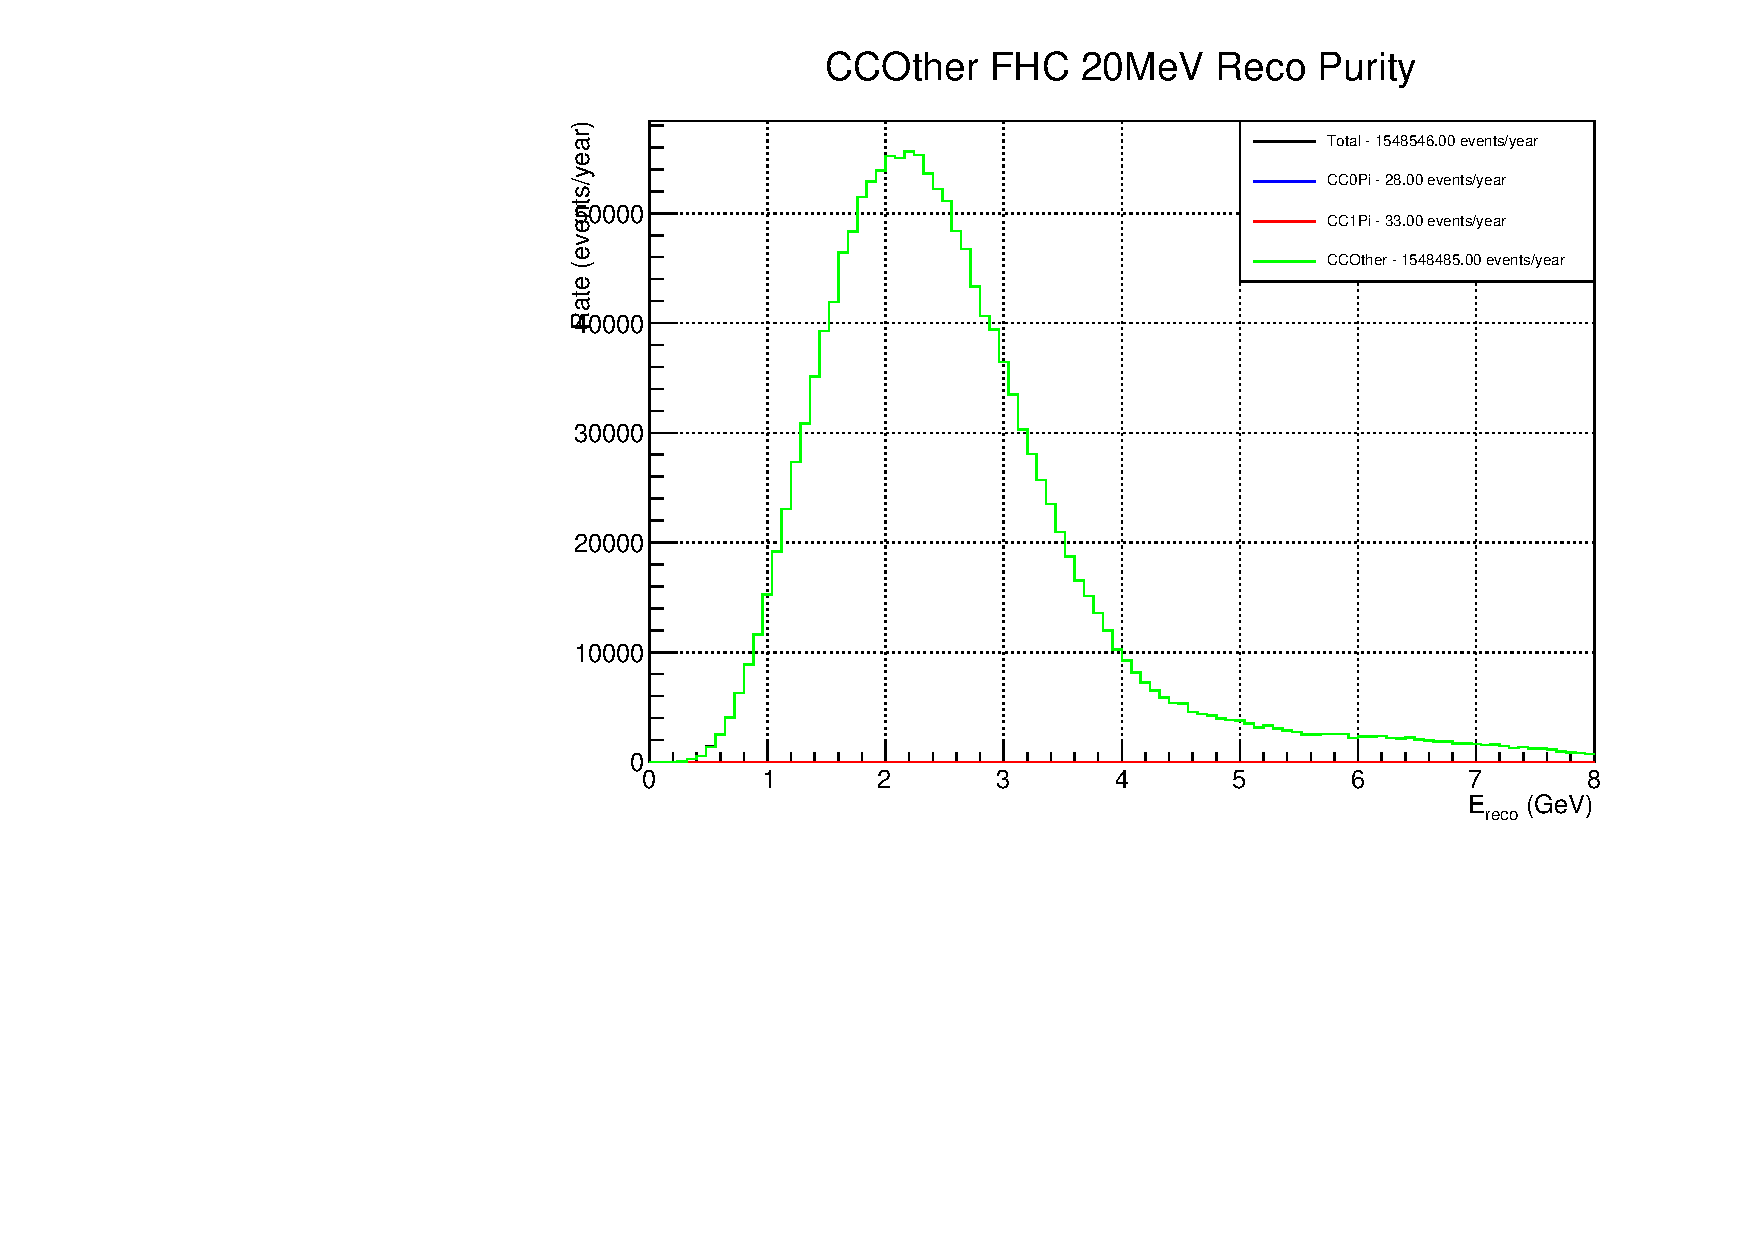
\includegraphics[width=0.245\textwidth]{plots/purity/CCOther_FHC_20MeV.pdf}
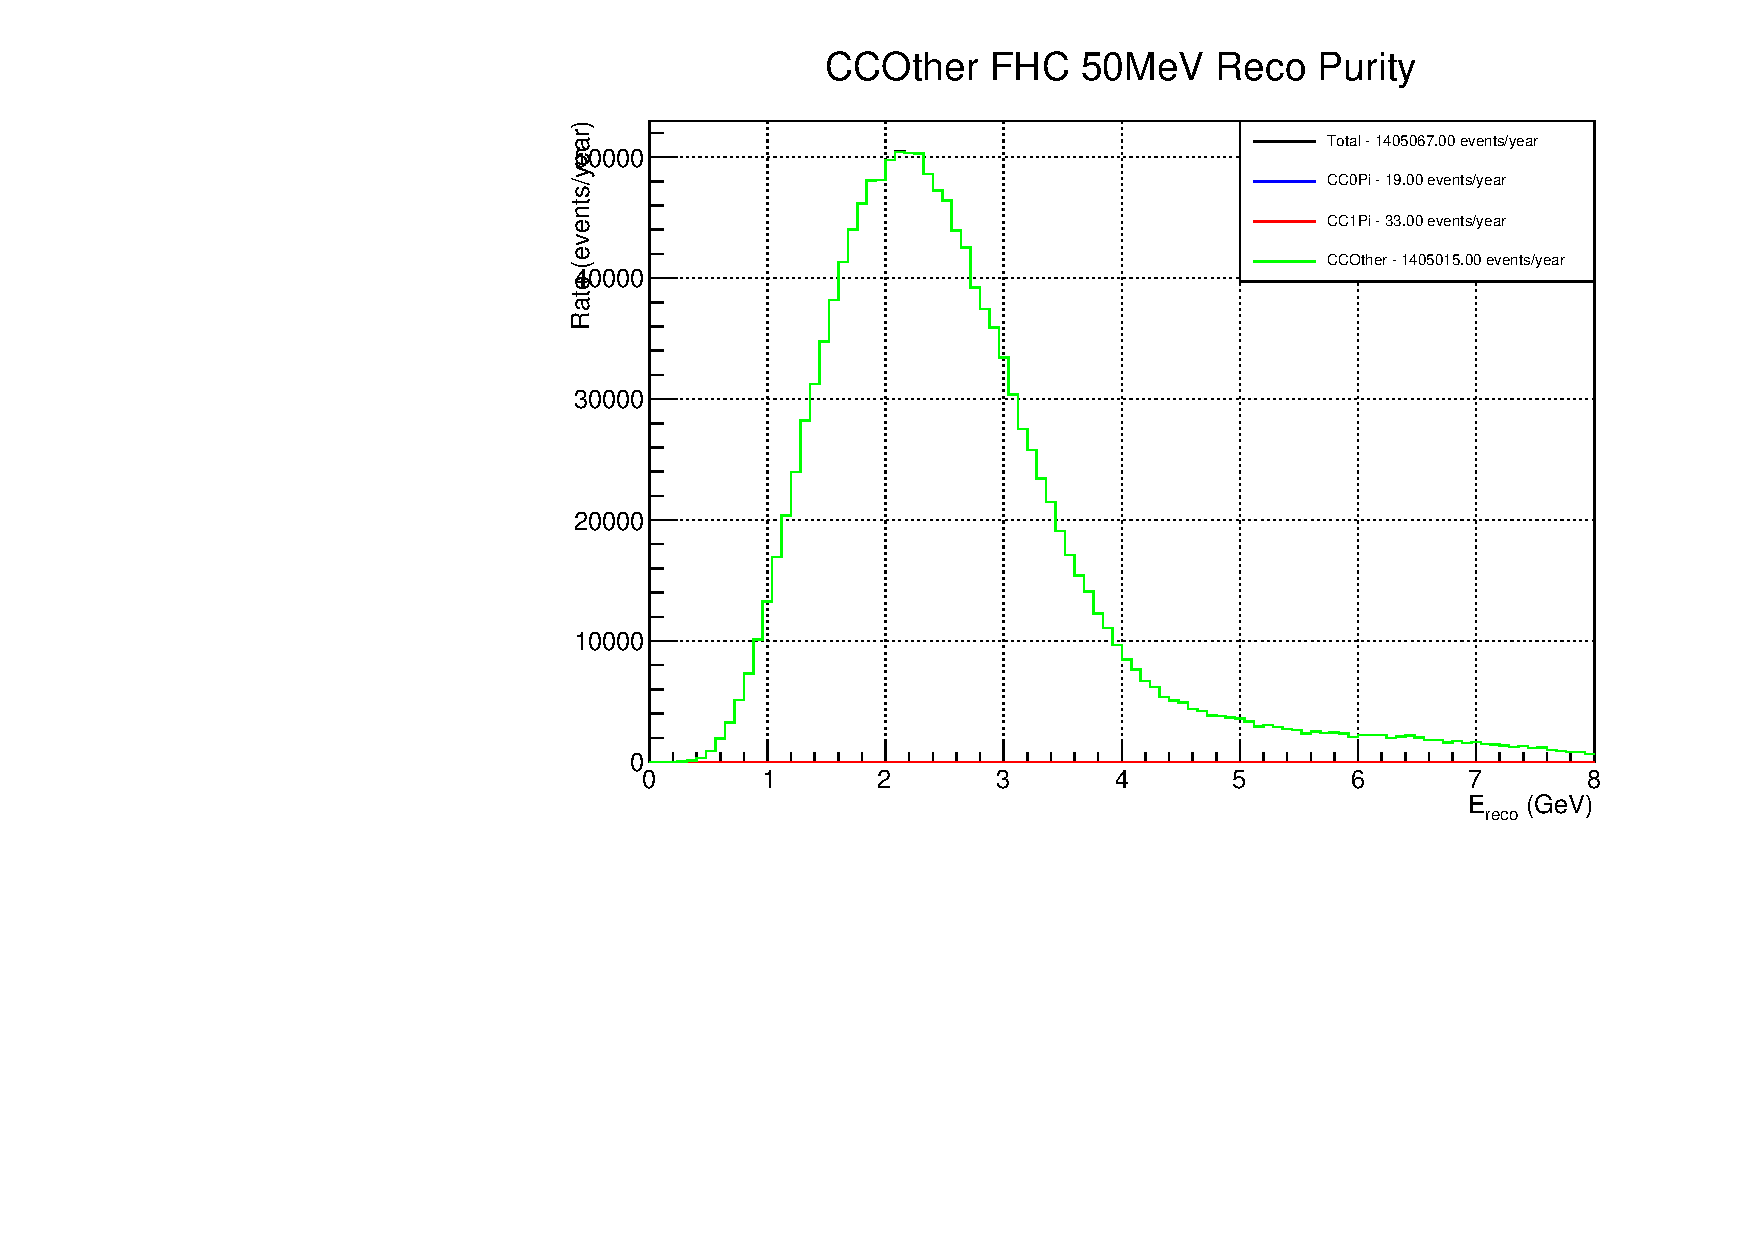
\includegraphics[width=0.245\textwidth]{plots/purity/CCOther_FHC_50MeV.pdf}

\end{center}


\subsection{RHC}

\subsubsection{CC0Pi}

\begin{center}

\includegraphics[width=0.245\textwidth]{plots/purity/CC0Pi_RHC_No_Threshold.pdf}
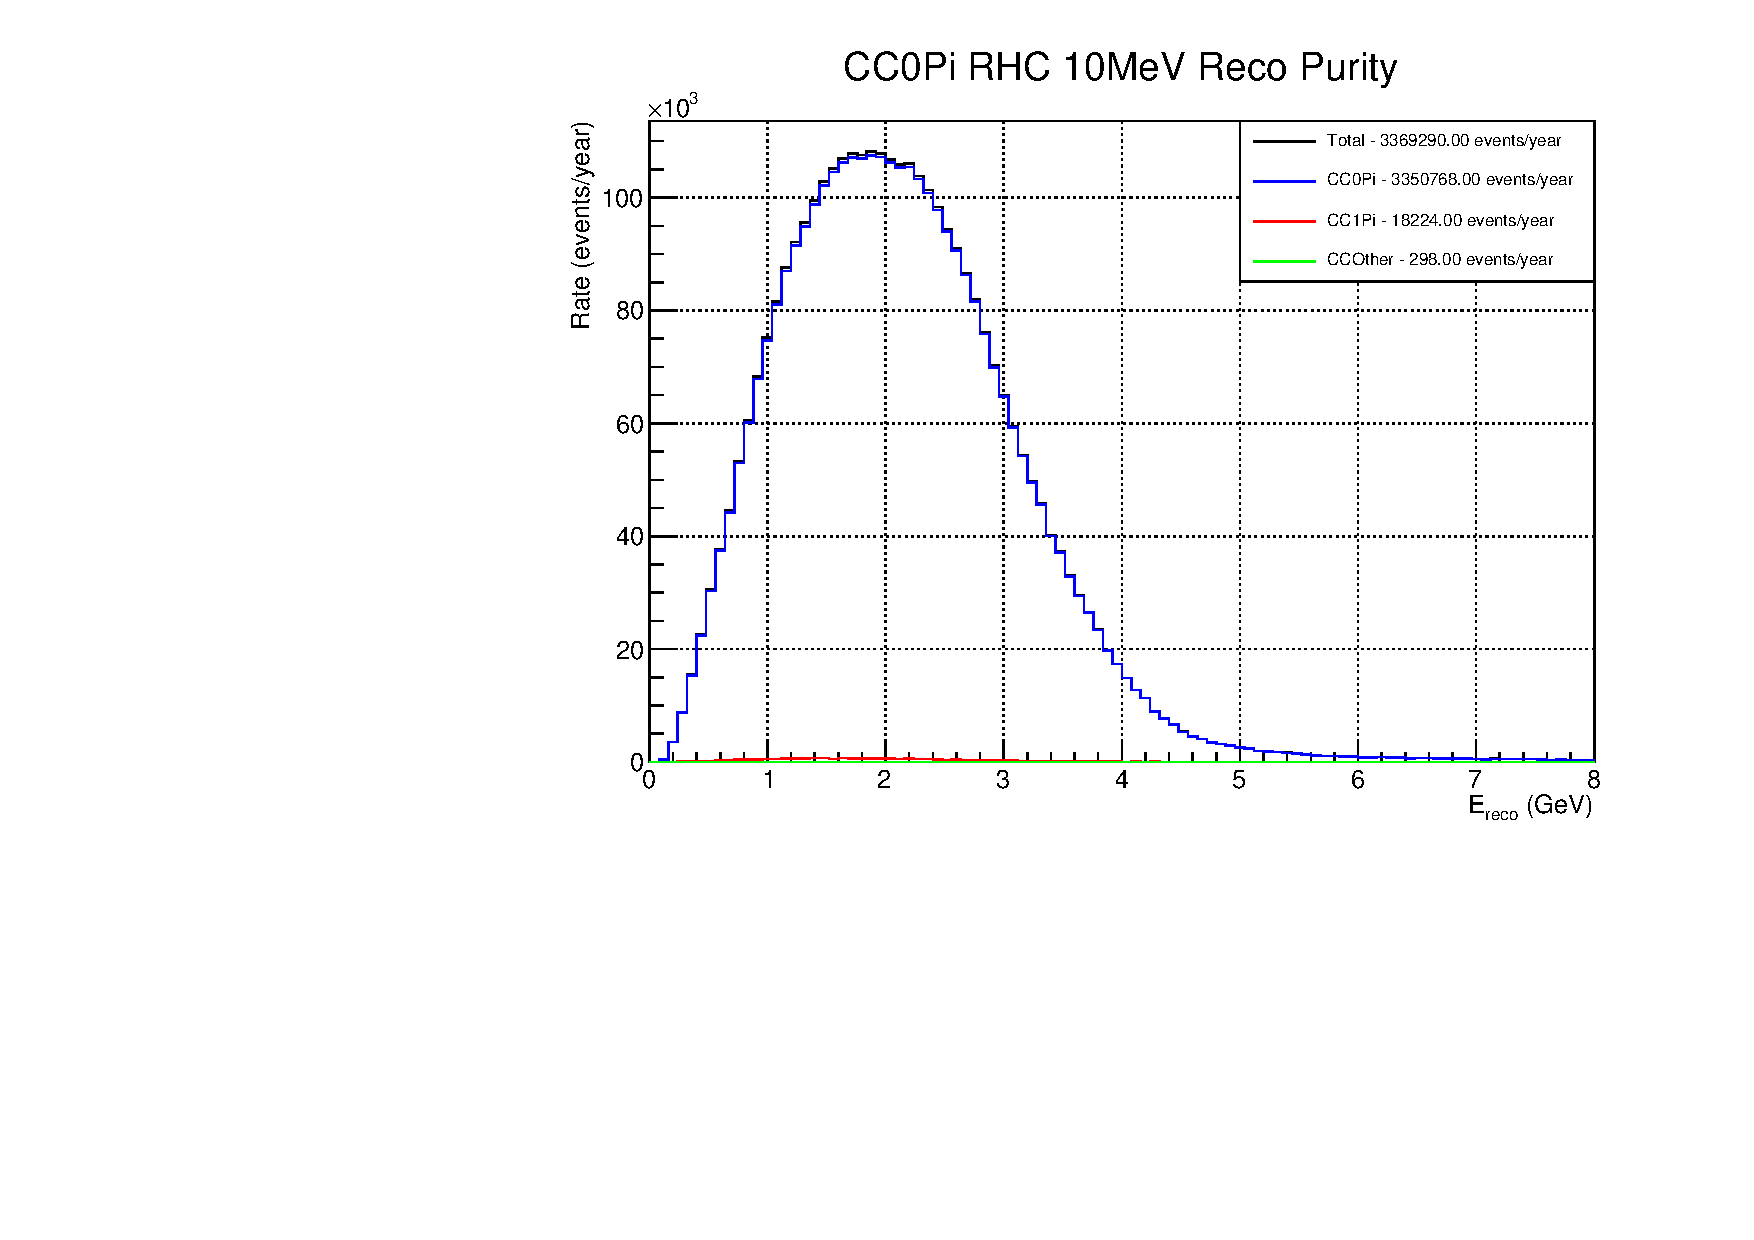
\includegraphics[width=0.245\textwidth]{plots/purity/CC0Pi_RHC_10MeV.pdf} 
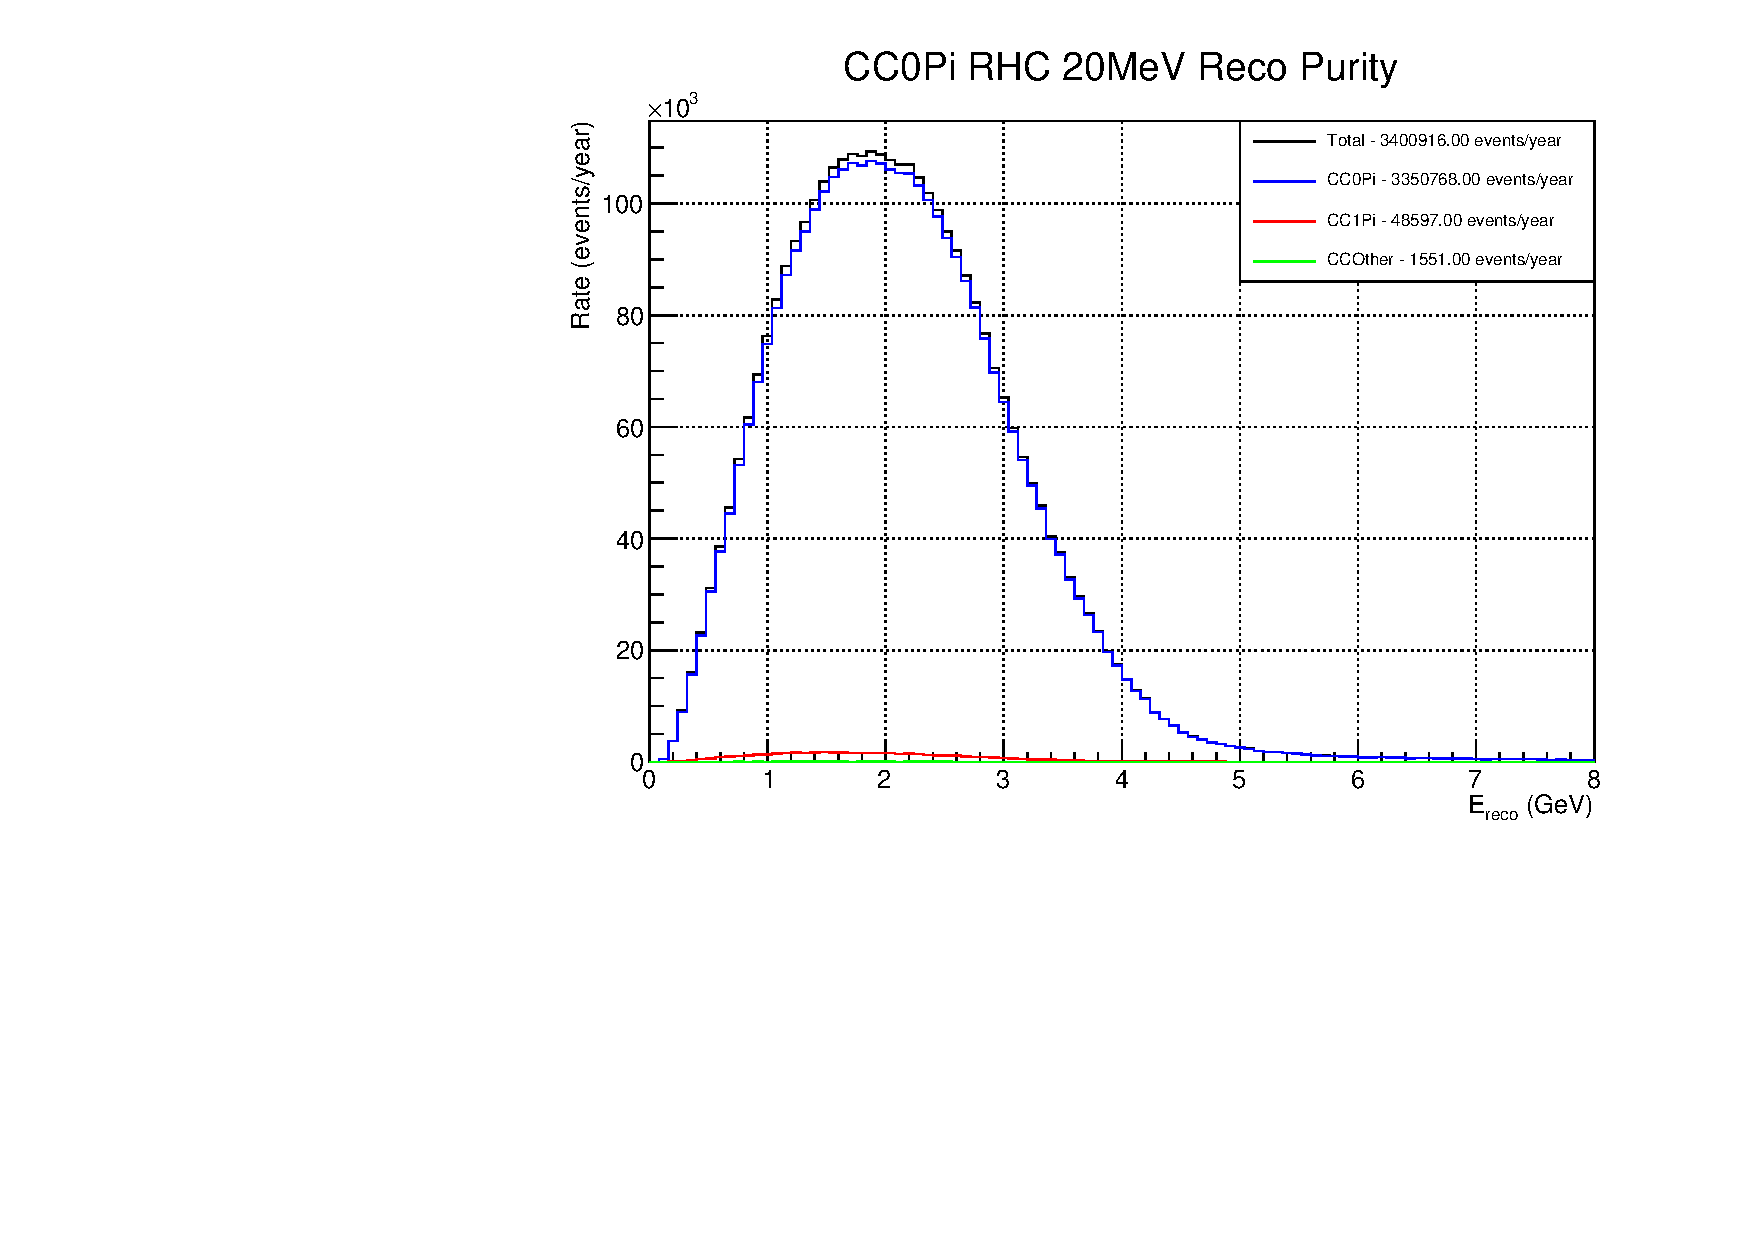
\includegraphics[width=0.245\textwidth]{plots/purity/CC0Pi_RHC_20MeV.pdf}
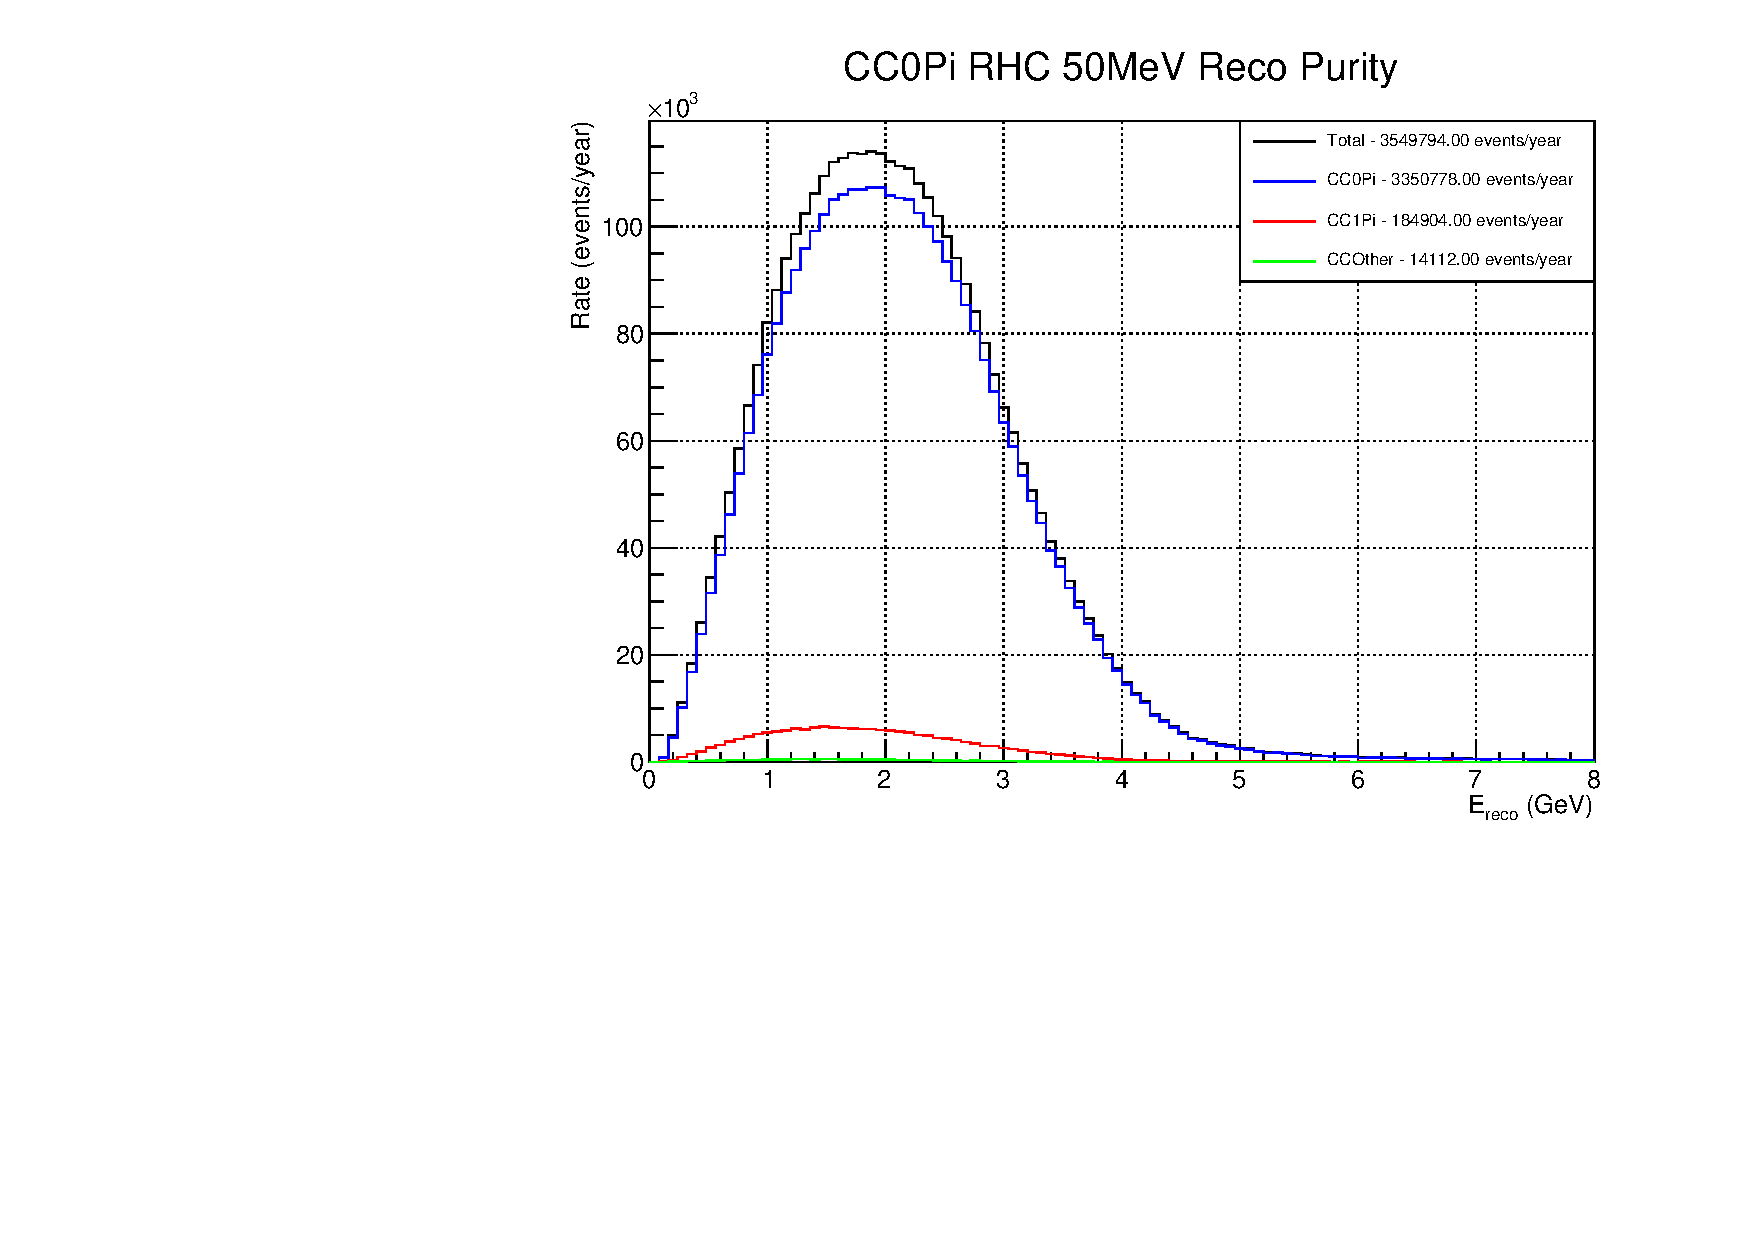
\includegraphics[width=0.245\textwidth]{plots/purity/CC0Pi_RHC_50MeV.pdf}

\end{center}

\subsubsection{CC1Pi}

\begin{center}

\includegraphics[width=0.245\textwidth]{plots/purity/CC1Pi_RHC_No_Threshold.pdf}
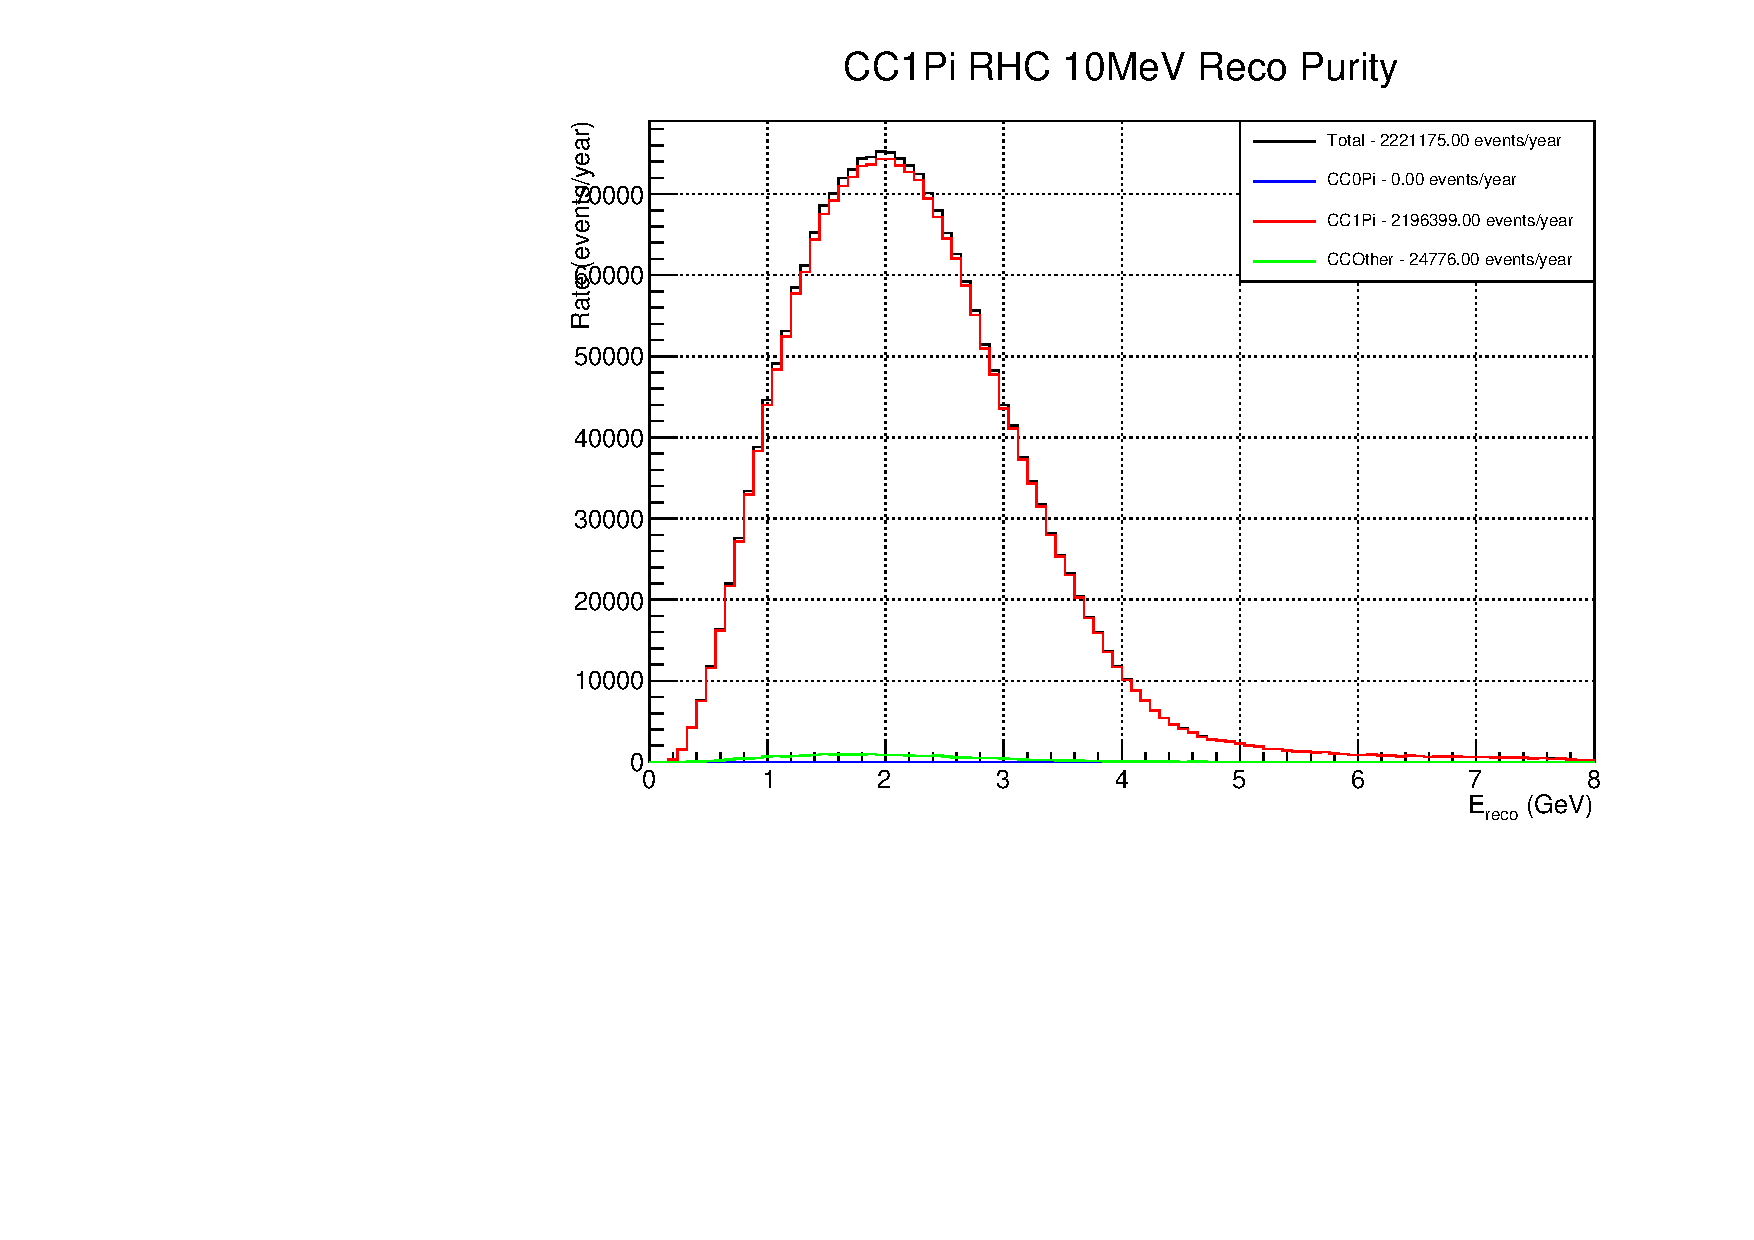
\includegraphics[width=0.245\textwidth]{plots/purity/CC1Pi_RHC_10MeV.pdf} 
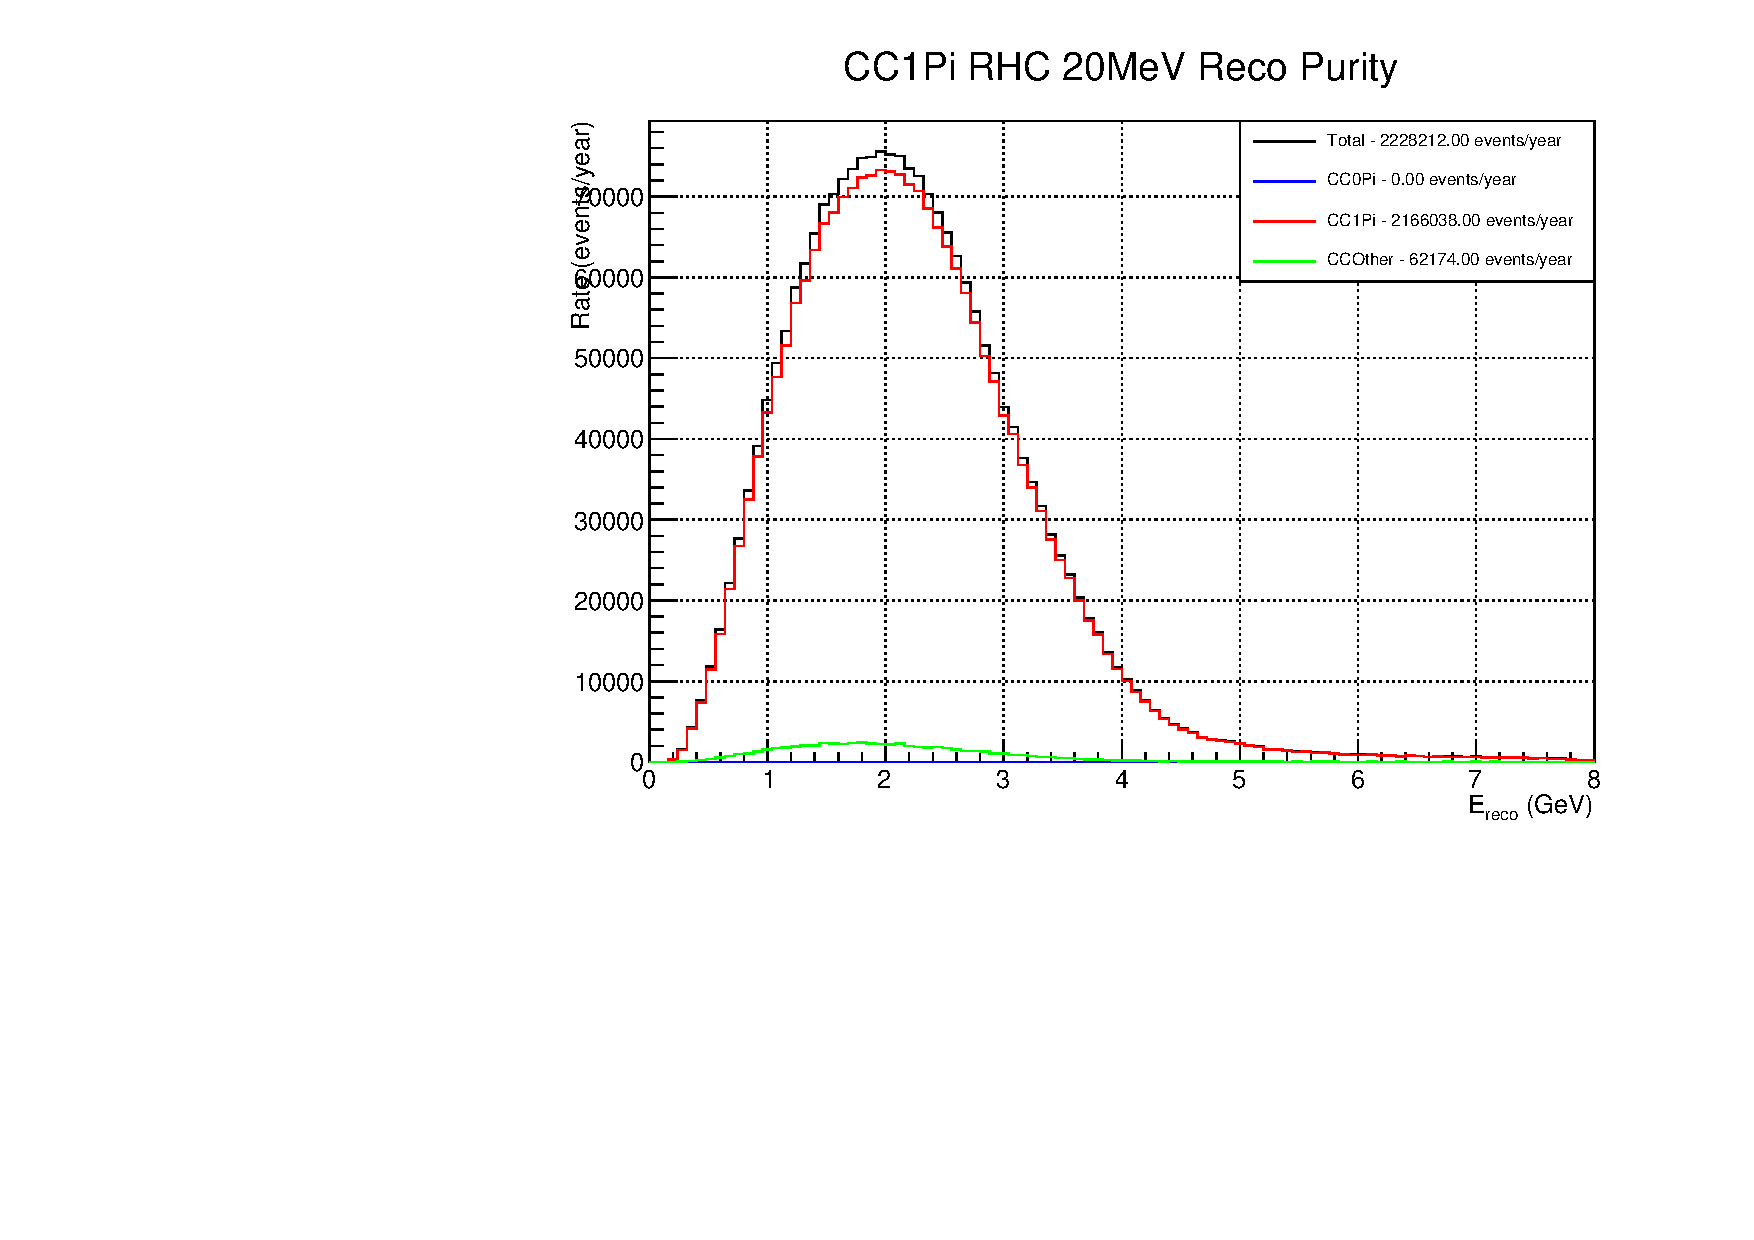
\includegraphics[width=0.245\textwidth]{plots/purity/CC1Pi_RHC_20MeV.pdf}
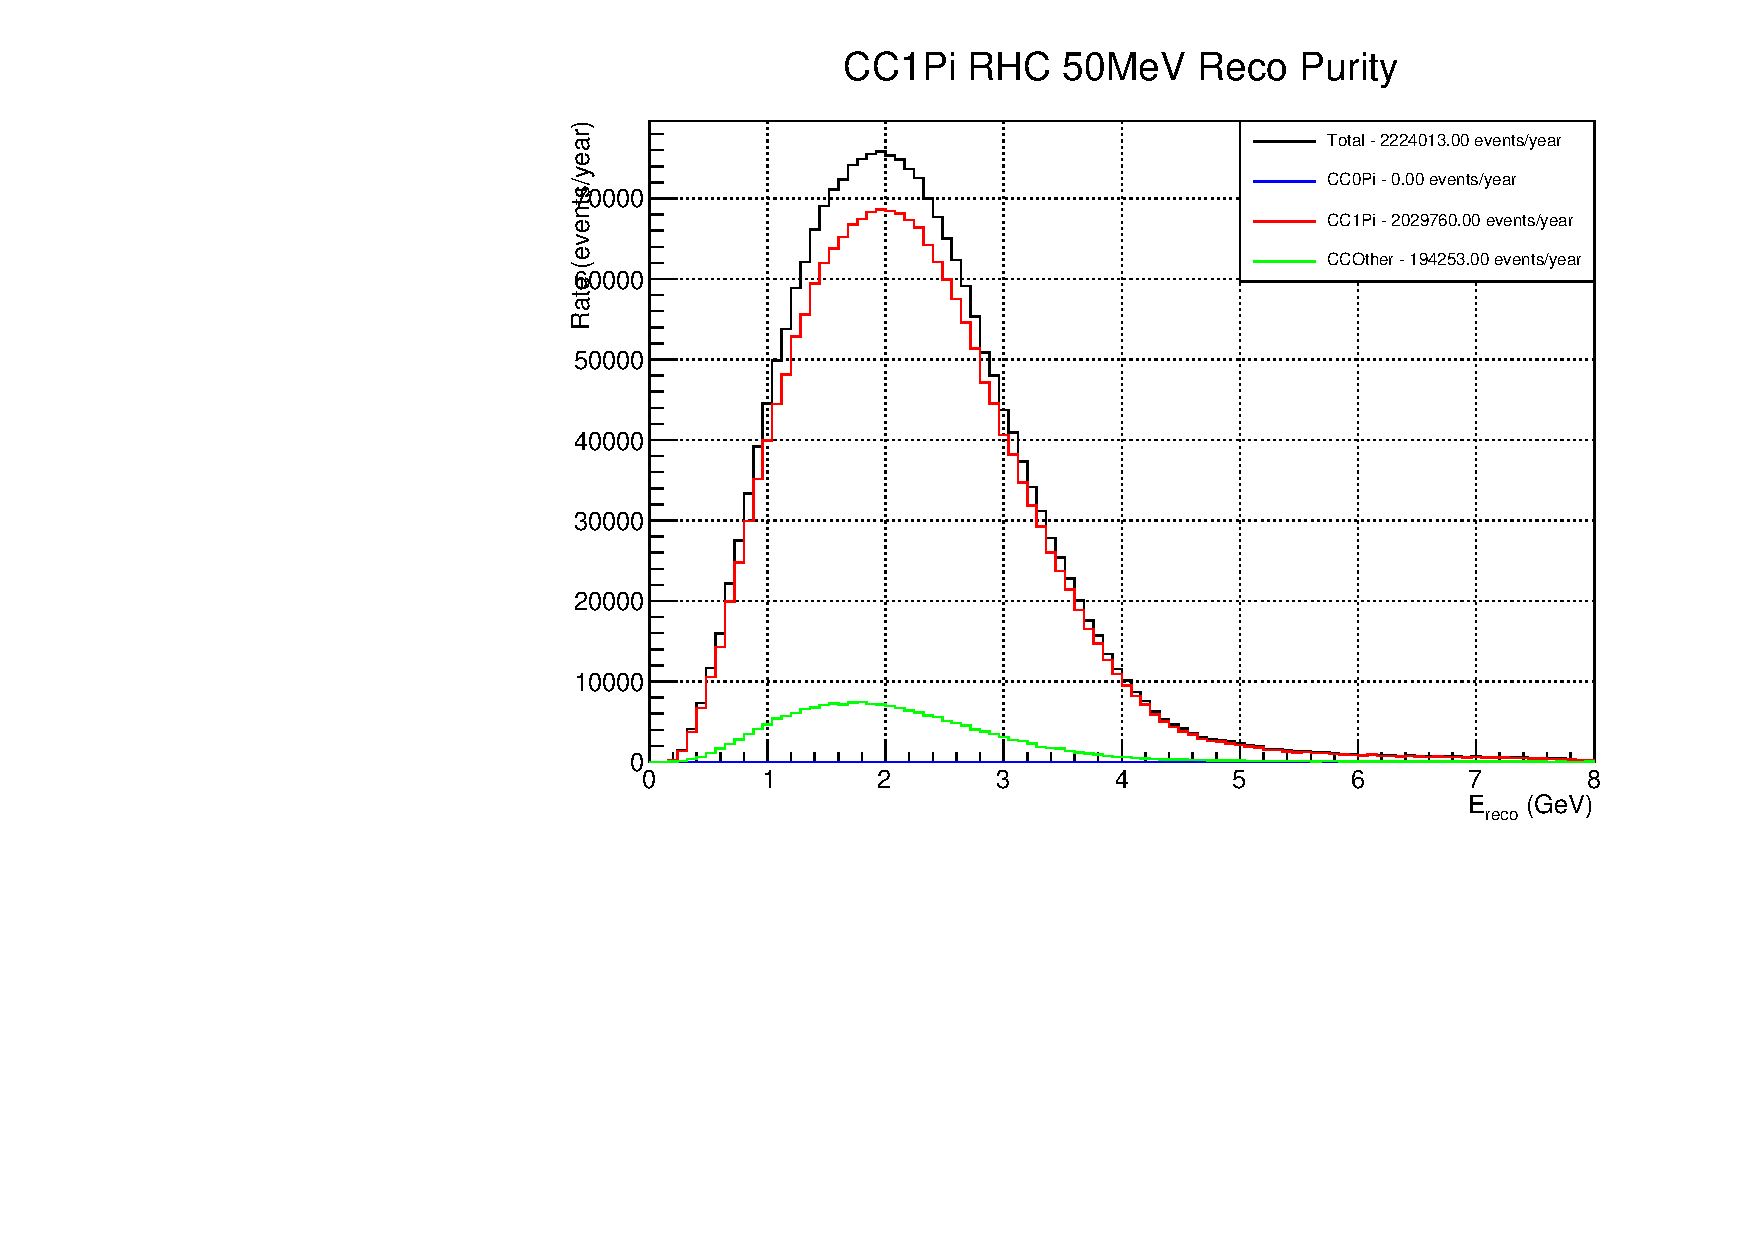
\includegraphics[width=0.245\textwidth]{plots/purity/CC1Pi_RHC_50MeV.pdf}

\end{center}

\subsubsection{CCOther}

\begin{center}

\includegraphics[width=0.245\textwidth]{plots/purity/CCOther_RHC_No_Threshold.pdf}
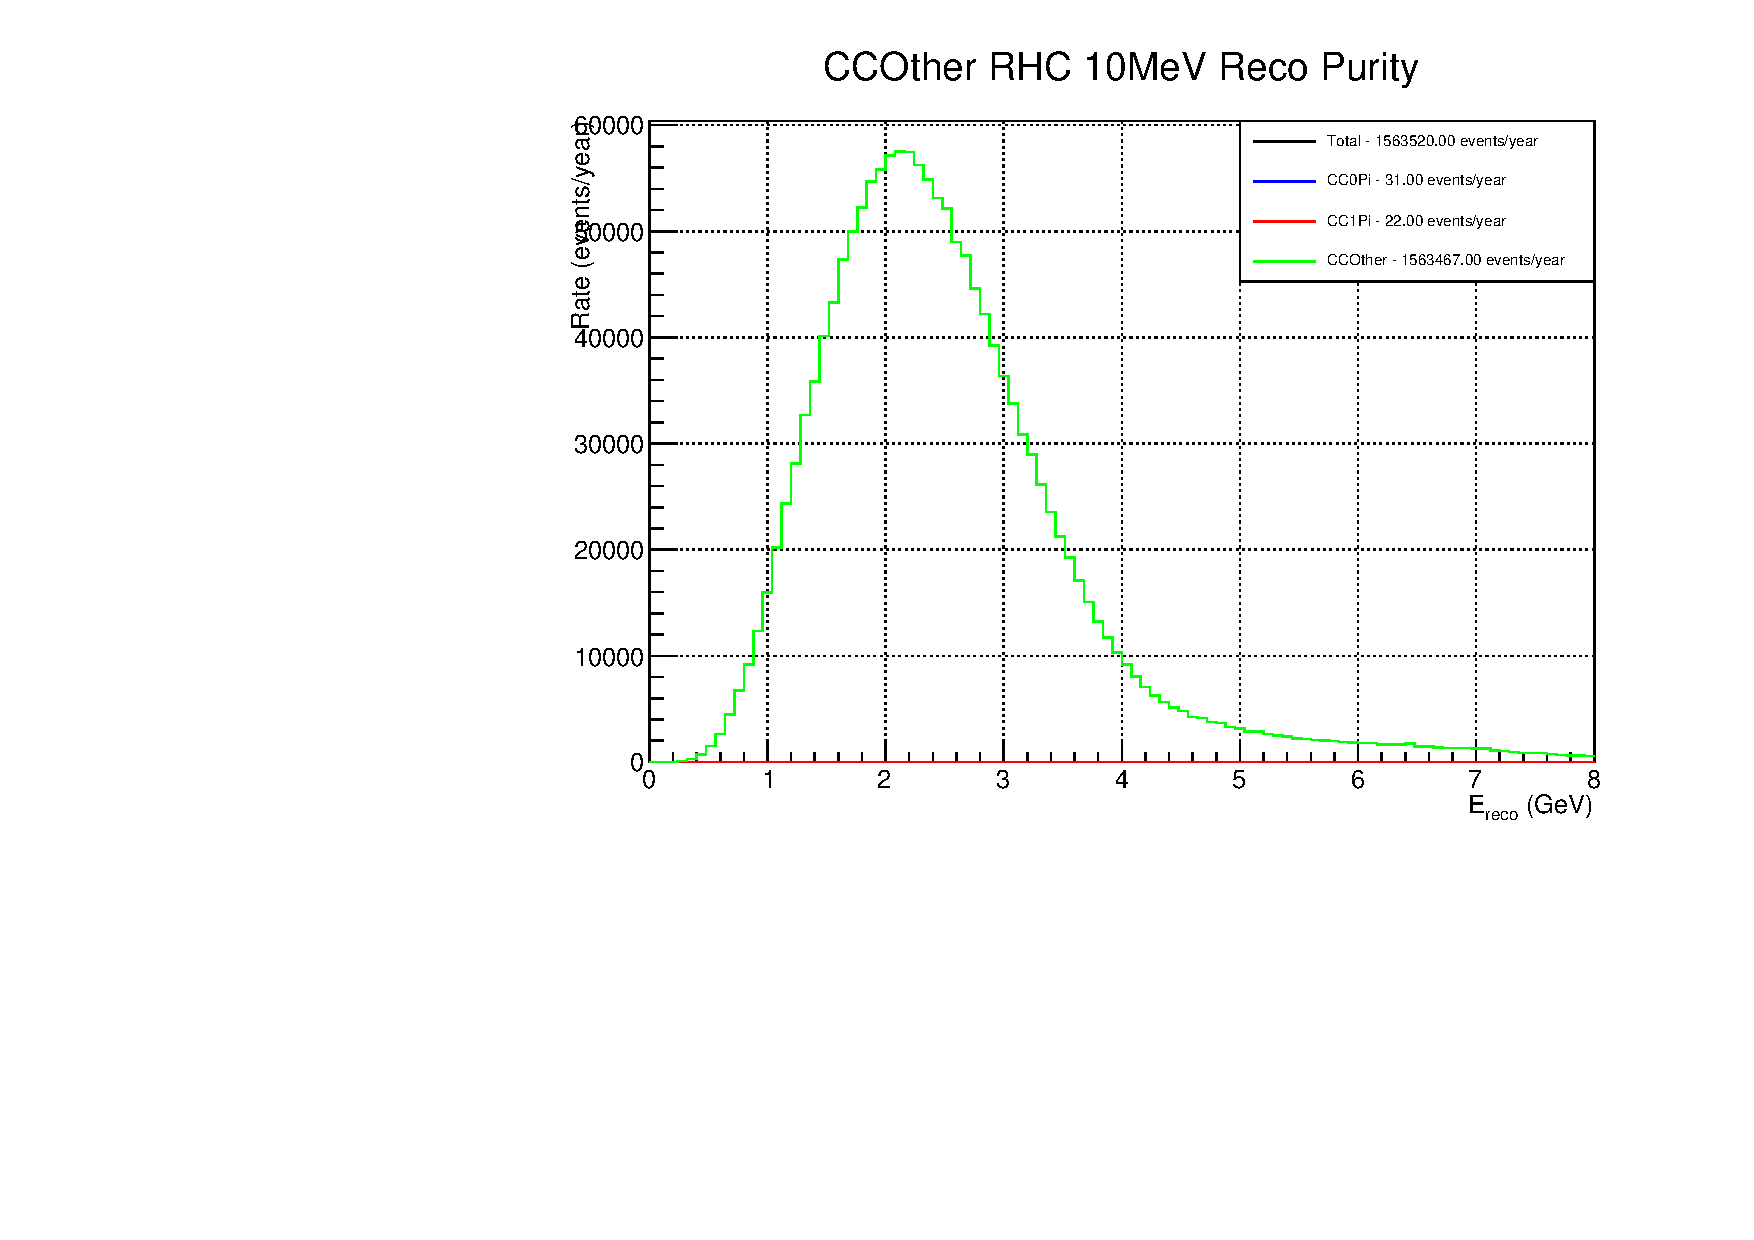
\includegraphics[width=0.245\textwidth]{plots/purity/CCOther_RHC_10MeV.pdf} 
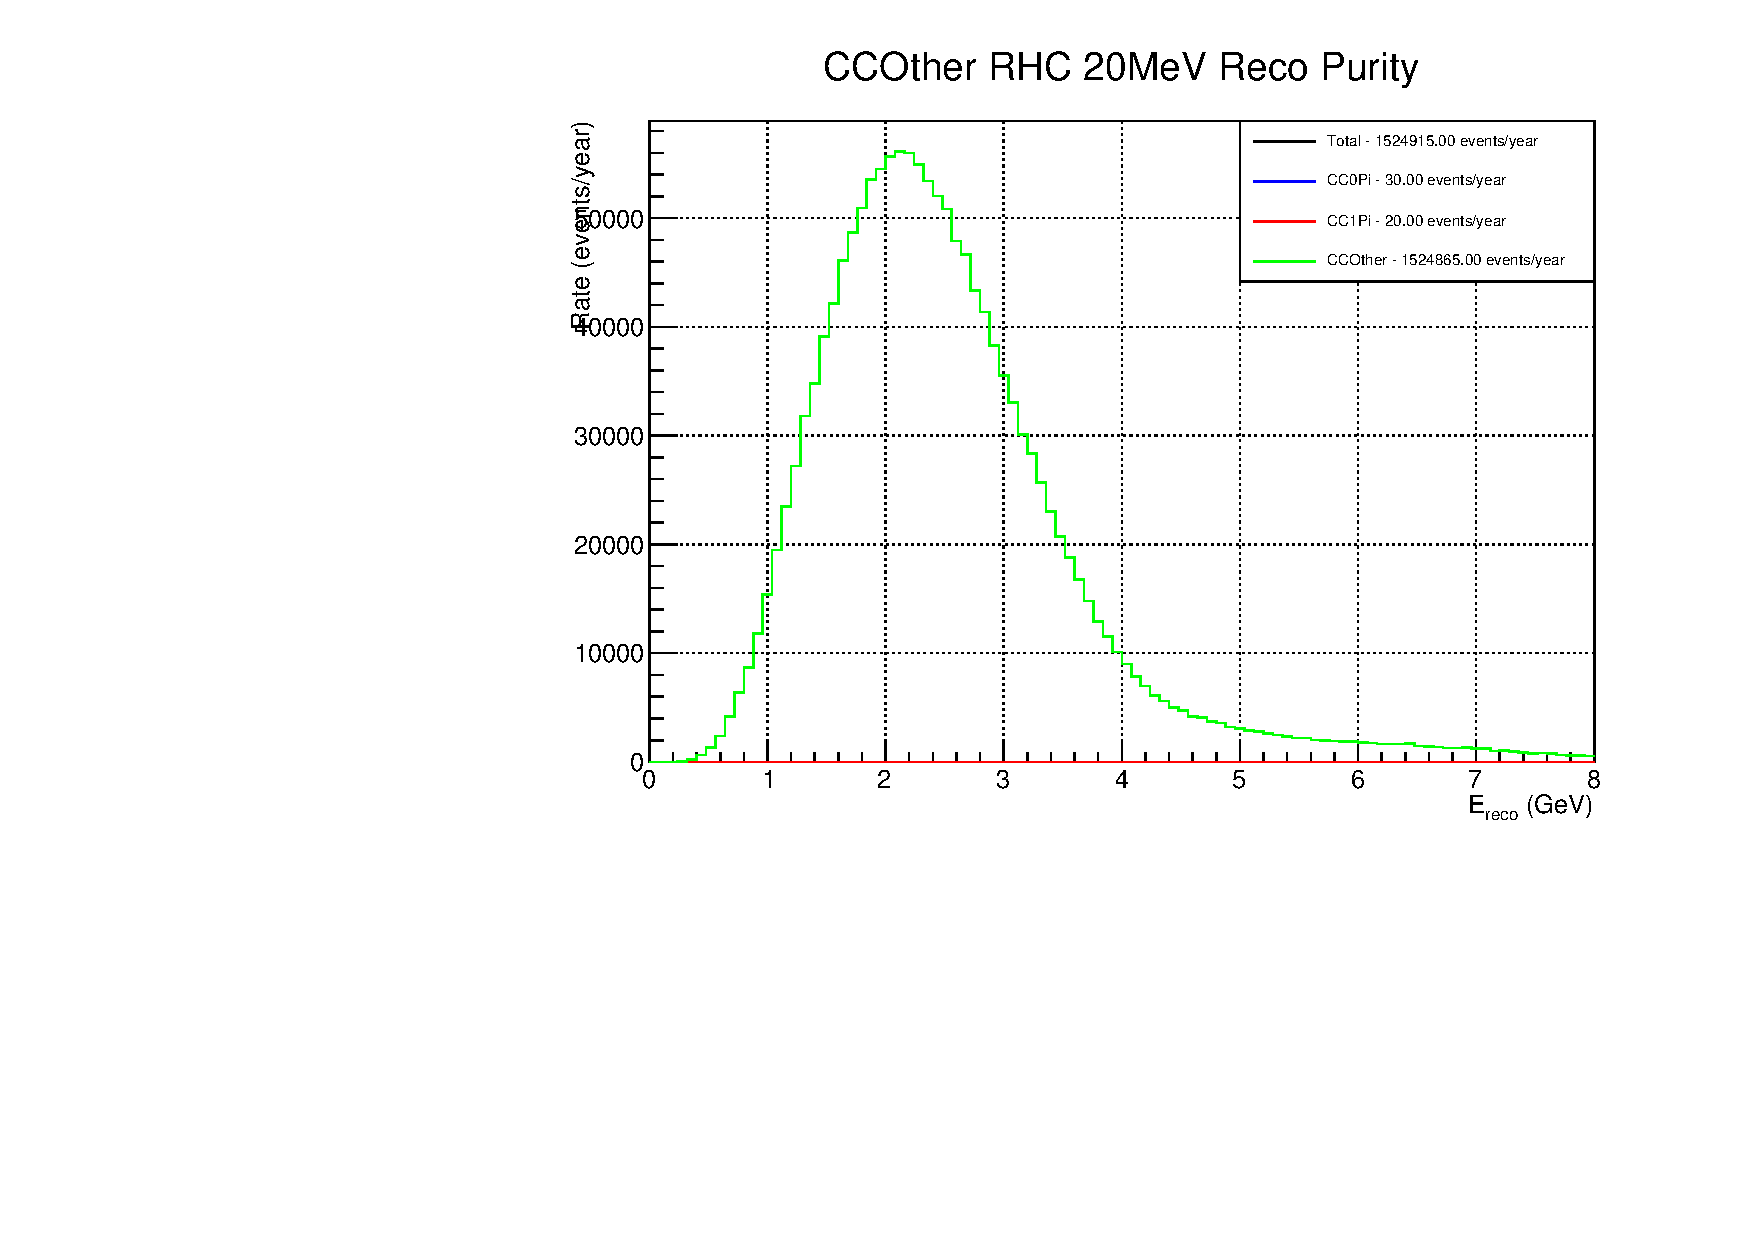
\includegraphics[width=0.245\textwidth]{plots/purity/CCOther_RHC_20MeV.pdf}
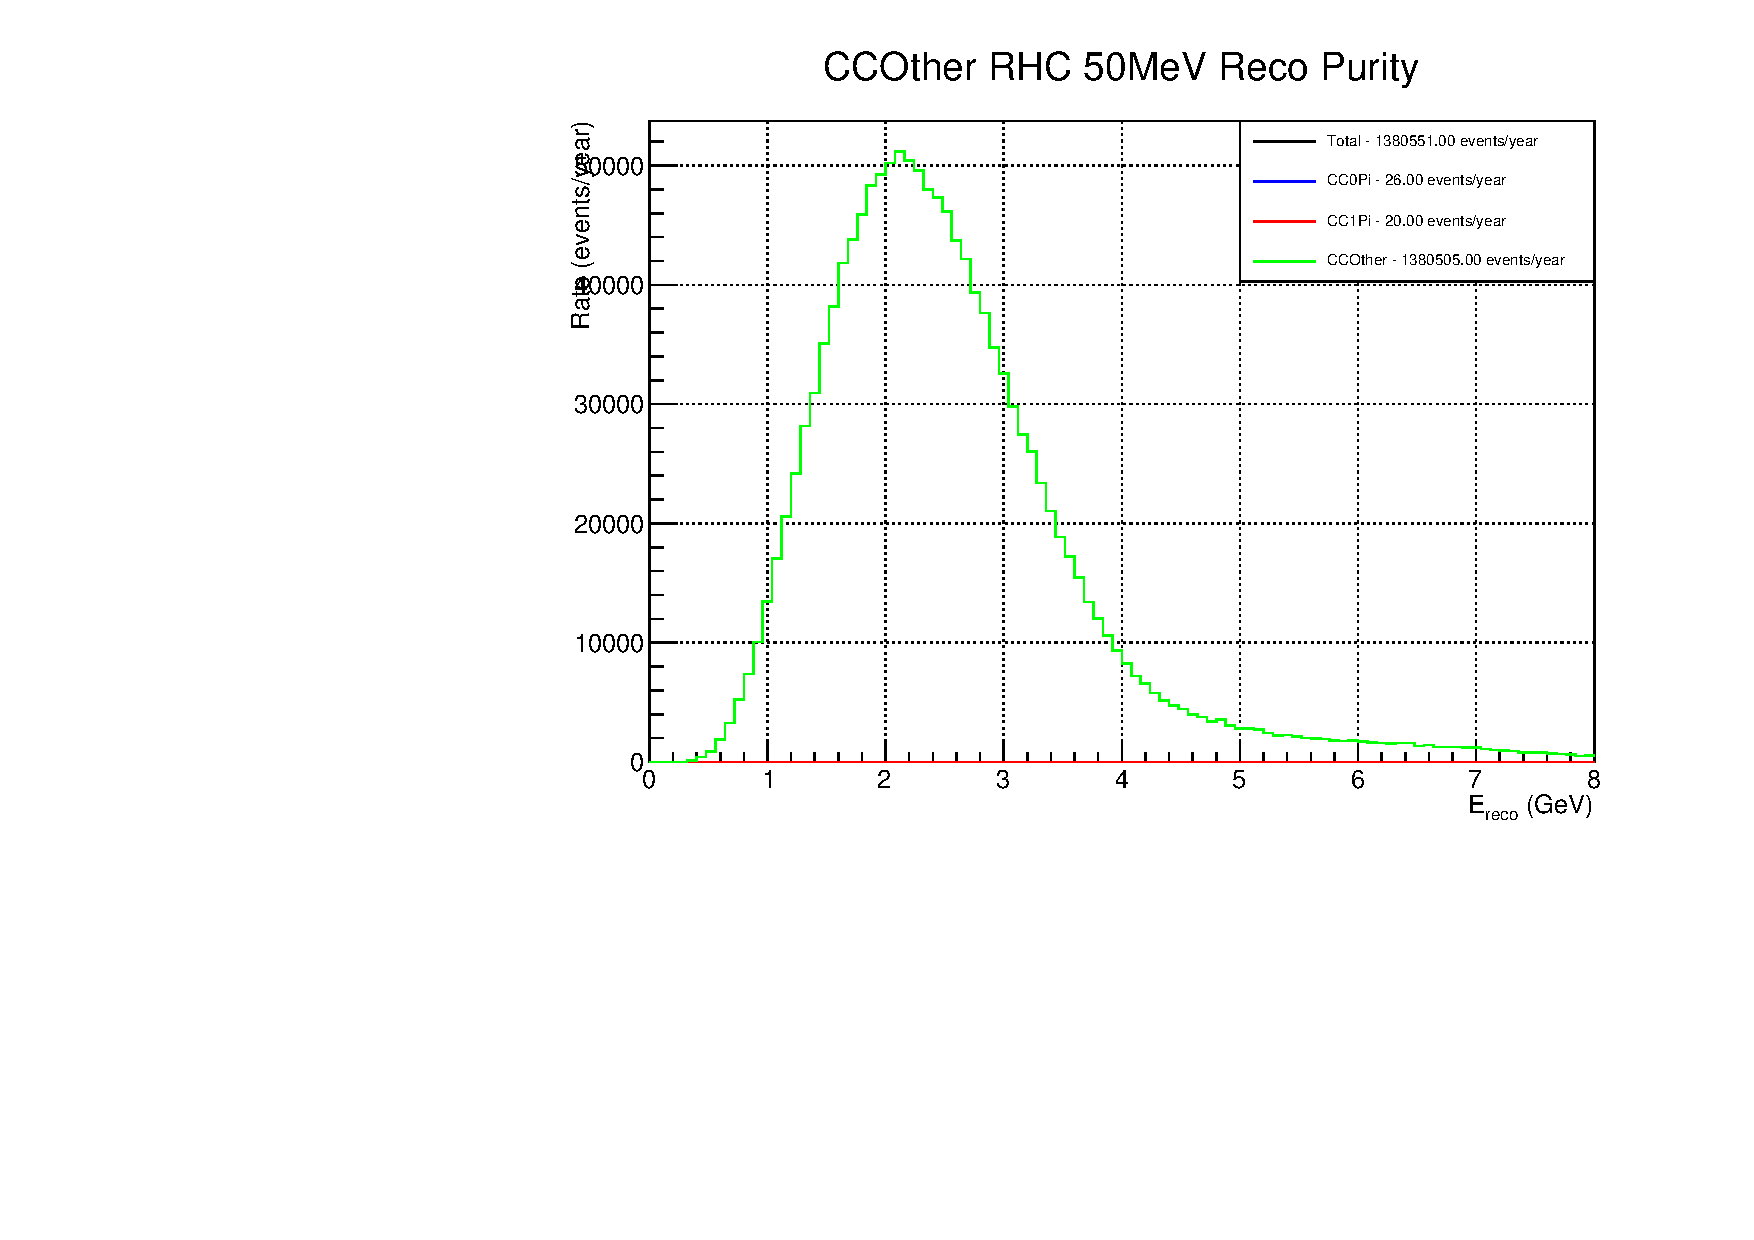
\includegraphics[width=0.245\textwidth]{plots/purity/CCOther_RHC_50MeV.pdf}

\end{center}


\section{Response Matrix}

\subsection{FHC}

\subsubsection{CCInc}

\textbf{No Threshold}

\begin{center}

  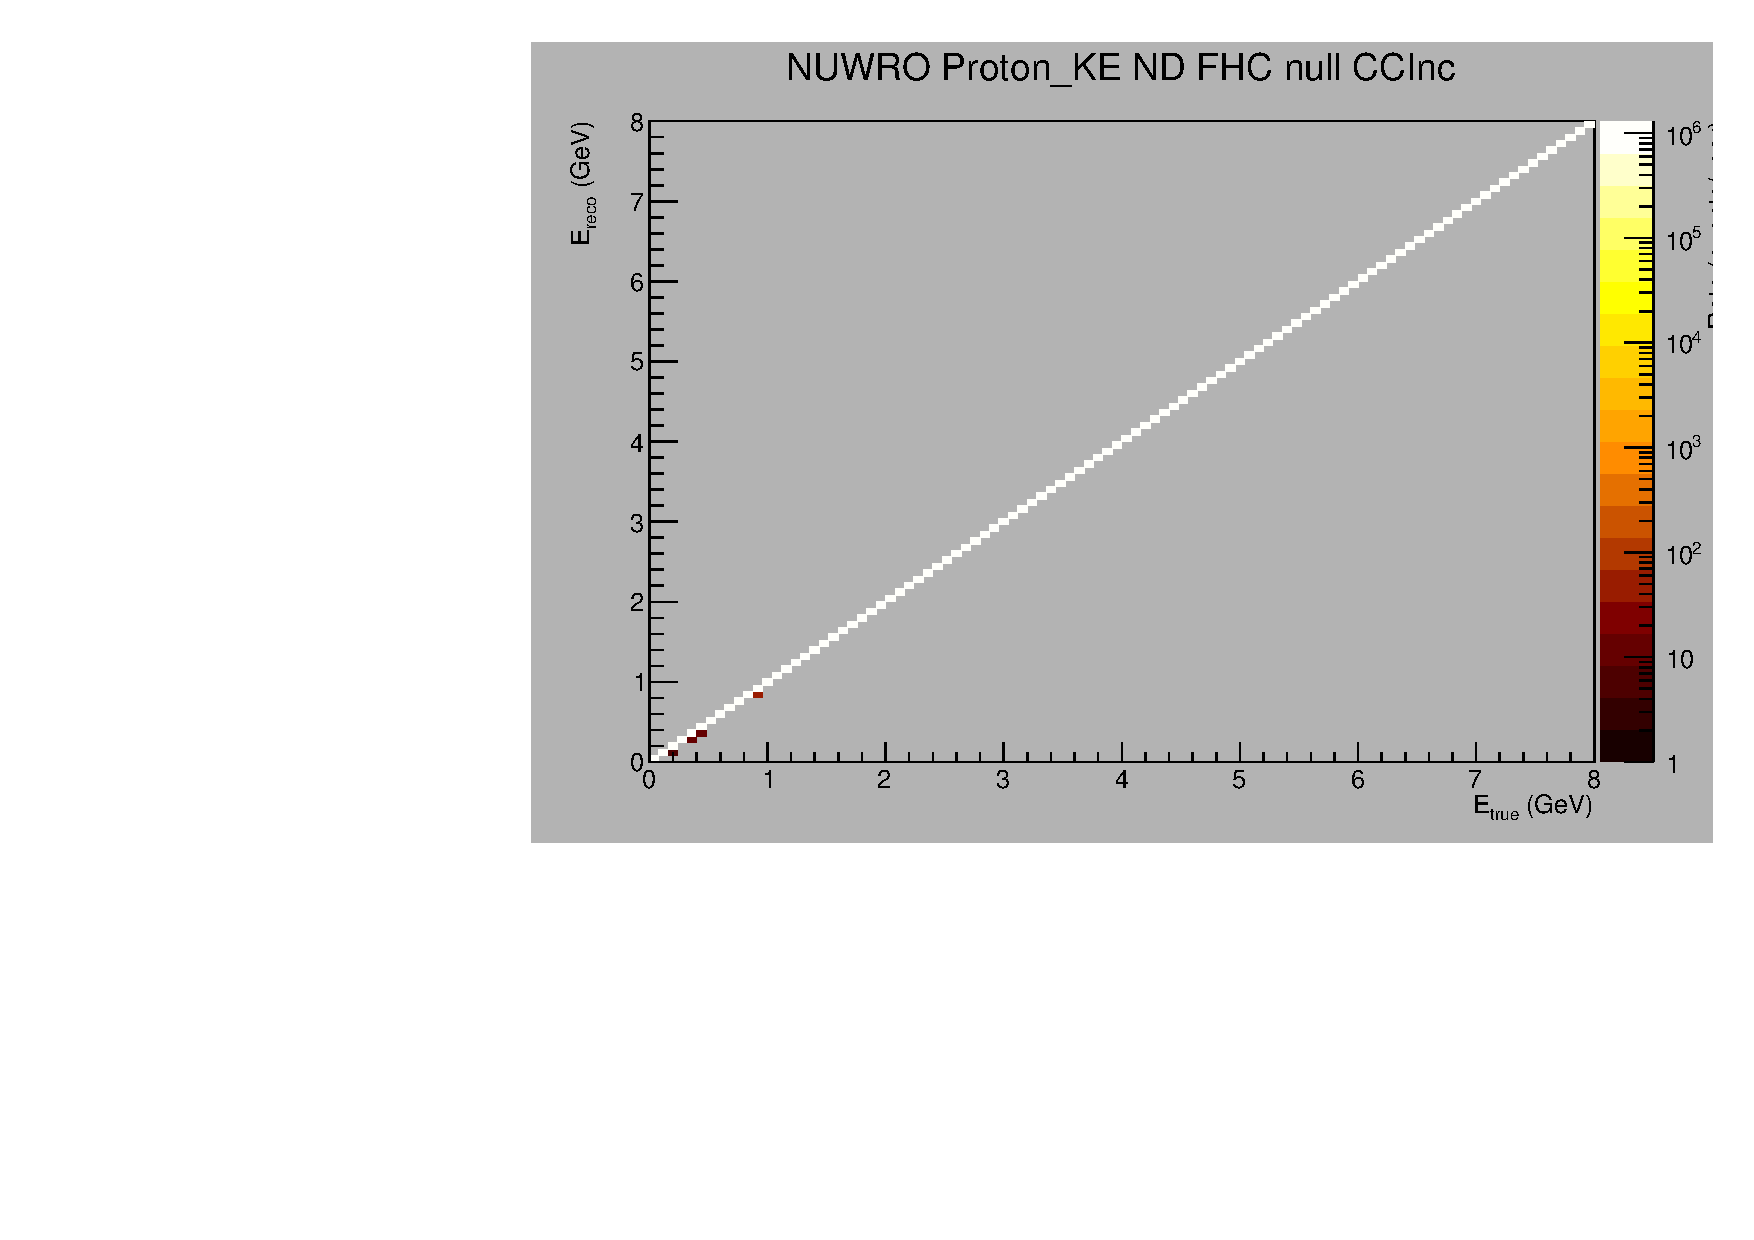
\includegraphics[width=0.245\textwidth]{plots/response_matrix/Proton_KE_FHC_CCInc_null.pdf}
  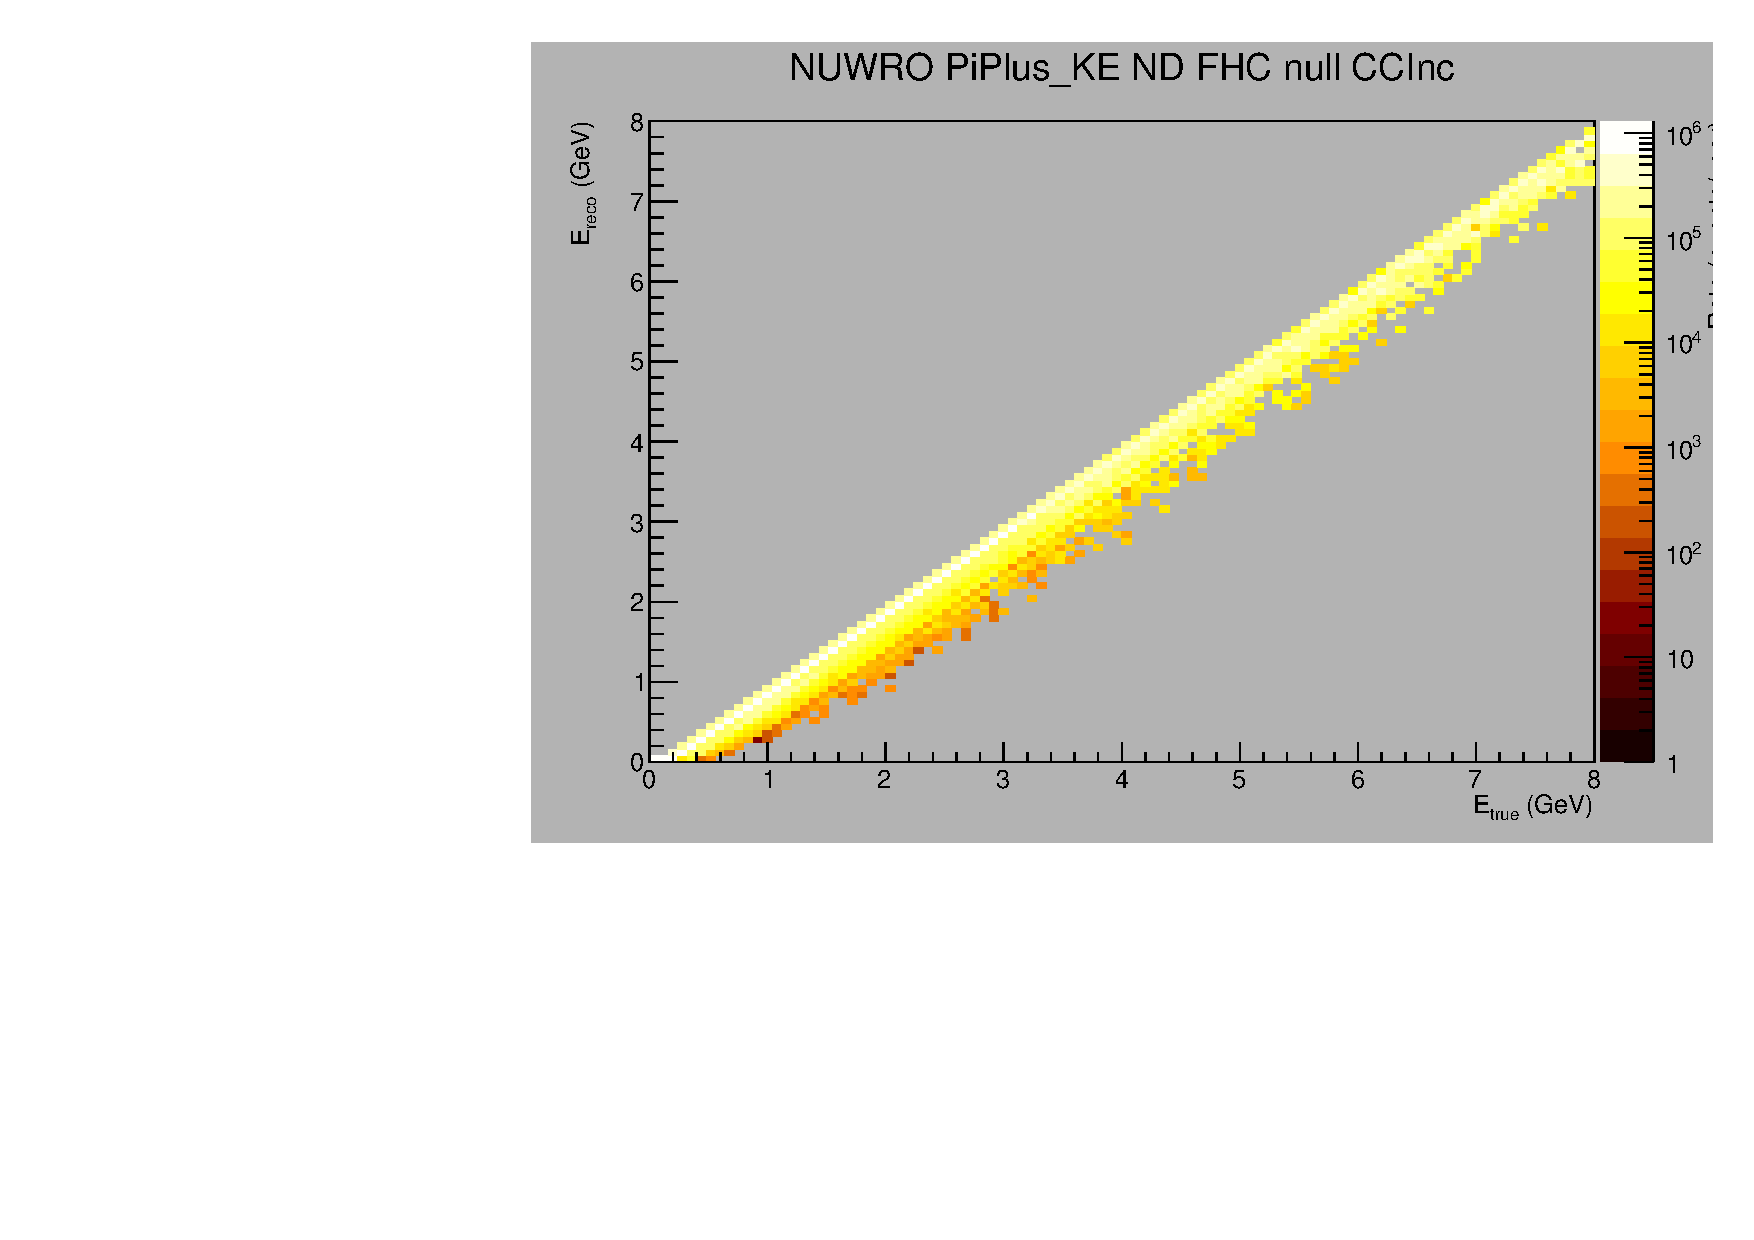
\includegraphics[width=0.245\textwidth]{plots/response_matrix/PiPlus_KE_FHC_CCInc_null.pdf}
  \includegraphics[width=0.245\textwidth]{plots/response_matrix/PiMinus_KE_FHC_CCInc_null.pdf}
  \includegraphics[width=0.245\textwidth]{plots/response_matrix/Charged_Pi_KE_FHC_CCInc_null.pdf}
  \includegraphics[width=0.245\textwidth]{plots/response_matrix/Pi0_KE_FHC_CCInc_null.pdf}
  \includegraphics[width=0.245\textwidth]{plots/response_matrix/Proton+Pion_KE_FHC_CCInc_null.pdf}
  \includegraphics[width=0.245\textwidth]{plots/response_matrix/Total_FHC_CCInc_null.pdf}
  \includegraphics[width=0.245\textwidth]{plots/response_matrix/Hadrons_FHC_CCInc_null.pdf}

\end{center}

\textbf{10 MeV Threshold}

\begin{center}

  \includegraphics[width=0.245\textwidth]{plots/response_matrix/Proton_KE_FHC_CCInc_10MeV.pdf}
  \includegraphics[width=0.245\textwidth]{plots/response_matrix/PiPlus_KE_FHC_CCInc_10MeV.pdf}
  \includegraphics[width=0.245\textwidth]{plots/response_matrix/PiMinus_KE_FHC_CCInc_10MeV.pdf}
  \includegraphics[width=0.245\textwidth]{plots/response_matrix/Charged_Pi_KE_FHC_CCInc_10MeV.pdf}
  \includegraphics[width=0.245\textwidth]{plots/response_matrix/Pi0_KE_FHC_CCInc_10MeV.pdf}
  \includegraphics[width=0.245\textwidth]{plots/response_matrix/Proton+Pion_KE_FHC_CCInc_10MeV.pdf}
  \includegraphics[width=0.245\textwidth]{plots/response_matrix/Total_FHC_CCInc_10MeV.pdf}
  \includegraphics[width=0.245\textwidth]{plots/response_matrix/Hadrons_FHC_CCInc_10MeV.pdf}

\end{center}

\textbf{20 MeV Threshold}

\begin{center}

  \includegraphics[width=0.245\textwidth]{plots/response_matrix/Proton_KE_FHC_CCInc_20MeV.pdf}
  \includegraphics[width=0.245\textwidth]{plots/response_matrix/PiPlus_KE_FHC_CCInc_20MeV.pdf}
  \includegraphics[width=0.245\textwidth]{plots/response_matrix/PiMinus_KE_FHC_CCInc_20MeV.pdf}
  \includegraphics[width=0.245\textwidth]{plots/response_matrix/Charged_Pi_KE_FHC_CCInc_20MeV.pdf}
  \includegraphics[width=0.245\textwidth]{plots/response_matrix/Pi0_KE_FHC_CCInc_20MeV.pdf}
  \includegraphics[width=0.245\textwidth]{plots/response_matrix/Proton+Pion_KE_FHC_CCInc_20MeV.pdf}
  \includegraphics[width=0.245\textwidth]{plots/response_matrix/Total_FHC_CCInc_20MeV.pdf}
  \includegraphics[width=0.245\textwidth]{plots/response_matrix/Hadrons_FHC_CCInc_20MeV.pdf}

\end{center}

\textbf{50 MeV Threshold}

\begin{center}

  \includegraphics[width=0.245\textwidth]{plots/response_matrix/Proton_KE_FHC_CCInc_50MeV.pdf}
  \includegraphics[width=0.245\textwidth]{plots/response_matrix/PiPlus_KE_FHC_CCInc_50MeV.pdf}
  \includegraphics[width=0.245\textwidth]{plots/response_matrix/PiMinus_KE_FHC_CCInc_50MeV.pdf}
  \includegraphics[width=0.245\textwidth]{plots/response_matrix/Charged_Pi_KE_FHC_CCInc_50MeV.pdf}
  \includegraphics[width=0.245\textwidth]{plots/response_matrix/Pi0_KE_FHC_CCInc_50MeV.pdf}
  \includegraphics[width=0.245\textwidth]{plots/response_matrix/Proton+Pion_KE_FHC_CCInc_50MeV.pdf}
  \includegraphics[width=0.245\textwidth]{plots/response_matrix/Total_FHC_CCInc_50MeV.pdf}
  \includegraphics[width=0.245\textwidth]{plots/response_matrix/Hadrons_FHC_CCInc_50MeV.pdf}

\end{center}

\subsubsection{CC0Pi}

\textbf{No Threshold}

\begin{center}

  \includegraphics[width=0.245\textwidth]{plots/response_matrix/Proton_KE_FHC_CC0Pi_null.pdf}
  \includegraphics[width=0.245\textwidth]{plots/response_matrix/PiPlus_KE_FHC_CC0Pi_null.pdf}
  \includegraphics[width=0.245\textwidth]{plots/response_matrix/PiMinus_KE_FHC_CC0Pi_null.pdf}
  \includegraphics[width=0.245\textwidth]{plots/response_matrix/Charged_Pi_KE_FHC_CC0Pi_null.pdf}
  \includegraphics[width=0.245\textwidth]{plots/response_matrix/Pi0_KE_FHC_CC0Pi_null.pdf}
  \includegraphics[width=0.245\textwidth]{plots/response_matrix/Proton+Pion_KE_FHC_CC0Pi_null.pdf}
  \includegraphics[width=0.245\textwidth]{plots/response_matrix/Total_FHC_CC0Pi_null.pdf}
  \includegraphics[width=0.245\textwidth]{plots/response_matrix/Hadrons_FHC_CC0Pi_null.pdf}

\end{center}

\textbf{10 MeV Threshold}

\begin{center}

  \includegraphics[width=0.245\textwidth]{plots/response_matrix/Proton_KE_FHC_CC0Pi_10MeV.pdf}
  \includegraphics[width=0.245\textwidth]{plots/response_matrix/PiPlus_KE_FHC_CC0Pi_10MeV.pdf}
  \includegraphics[width=0.245\textwidth]{plots/response_matrix/PiMinus_KE_FHC_CC0Pi_10MeV.pdf}
  \includegraphics[width=0.245\textwidth]{plots/response_matrix/Charged_Pi_KE_FHC_CC0Pi_10MeV.pdf}
  \includegraphics[width=0.245\textwidth]{plots/response_matrix/Pi0_KE_FHC_CC0Pi_10MeV.pdf}
  \includegraphics[width=0.245\textwidth]{plots/response_matrix/Proton+Pion_KE_FHC_CC0Pi_10MeV.pdf}
  \includegraphics[width=0.245\textwidth]{plots/response_matrix/Total_FHC_CC0Pi_10MeV.pdf}
  \includegraphics[width=0.245\textwidth]{plots/response_matrix/Hadrons_FHC_CC0Pi_10MeV.pdf}

\end{center}

\textbf{20 MeV Threshold}

\begin{center}

  \includegraphics[width=0.245\textwidth]{plots/response_matrix/Proton_KE_FHC_CC0Pi_20MeV.pdf}
  \includegraphics[width=0.245\textwidth]{plots/response_matrix/PiPlus_KE_FHC_CC0Pi_20MeV.pdf}
  \includegraphics[width=0.245\textwidth]{plots/response_matrix/PiMinus_KE_FHC_CC0Pi_20MeV.pdf}
  \includegraphics[width=0.245\textwidth]{plots/response_matrix/Charged_Pi_KE_FHC_CC0Pi_20MeV.pdf}
  \includegraphics[width=0.245\textwidth]{plots/response_matrix/Pi0_KE_FHC_CC0Pi_20MeV.pdf}
  \includegraphics[width=0.245\textwidth]{plots/response_matrix/Proton+Pion_KE_FHC_CC0Pi_20MeV.pdf}
  \includegraphics[width=0.245\textwidth]{plots/response_matrix/Total_FHC_CC0Pi_20MeV.pdf}
  \includegraphics[width=0.245\textwidth]{plots/response_matrix/Hadrons_FHC_CC0Pi_20MeV.pdf}

\end{center}

\textbf{50 MeV Threshold}

\begin{center}

  \includegraphics[width=0.245\textwidth]{plots/response_matrix/Proton_KE_FHC_CC0Pi_50MeV.pdf}
  \includegraphics[width=0.245\textwidth]{plots/response_matrix/PiPlus_KE_FHC_CC0Pi_50MeV.pdf}
  \includegraphics[width=0.245\textwidth]{plots/response_matrix/PiMinus_KE_FHC_CC0Pi_50MeV.pdf}
  \includegraphics[width=0.245\textwidth]{plots/response_matrix/Charged_Pi_KE_FHC_CC0Pi_50MeV.pdf}
  \includegraphics[width=0.245\textwidth]{plots/response_matrix/Pi0_KE_FHC_CC0Pi_50MeV.pdf}
  \includegraphics[width=0.245\textwidth]{plots/response_matrix/Proton+Pion_KE_FHC_CC0Pi_50MeV.pdf}
  \includegraphics[width=0.245\textwidth]{plots/response_matrix/Total_FHC_CC0Pi_50MeV.pdf}
  \includegraphics[width=0.245\textwidth]{plots/response_matrix/Hadrons_FHC_CC0Pi_50MeV.pdf}

\end{center}

\subsubsection{CC1Pi}

\textbf{No Threshold}

\begin{center}

  \includegraphics[width=0.245\textwidth]{plots/response_matrix/Proton_KE_FHC_CC1Pi_null.pdf}
  \includegraphics[width=0.245\textwidth]{plots/response_matrix/PiPlus_KE_FHC_CC1Pi_null.pdf}
  \includegraphics[width=0.245\textwidth]{plots/response_matrix/PiMinus_KE_FHC_CC1Pi_null.pdf}
  \includegraphics[width=0.245\textwidth]{plots/response_matrix/Charged_Pi_KE_FHC_CC1Pi_null.pdf}
  \includegraphics[width=0.245\textwidth]{plots/response_matrix/Pi0_KE_FHC_CC1Pi_null.pdf}
  \includegraphics[width=0.245\textwidth]{plots/response_matrix/Proton+Pion_KE_FHC_CC1Pi_null.pdf}
  \includegraphics[width=0.245\textwidth]{plots/response_matrix/Total_FHC_CC1Pi_null.pdf}
  \includegraphics[width=0.245\textwidth]{plots/response_matrix/Hadrons_FHC_CC1Pi_null.pdf}

\end{center}

\textbf{10 MeV Threshold}

\begin{center}

  \includegraphics[width=0.245\textwidth]{plots/response_matrix/Proton_KE_FHC_CC1Pi_10MeV.pdf}
  \includegraphics[width=0.245\textwidth]{plots/response_matrix/PiPlus_KE_FHC_CC1Pi_10MeV.pdf}
  \includegraphics[width=0.245\textwidth]{plots/response_matrix/PiMinus_KE_FHC_CC1Pi_10MeV.pdf}
  \includegraphics[width=0.245\textwidth]{plots/response_matrix/Charged_Pi_KE_FHC_CC1Pi_10MeV.pdf}
  \includegraphics[width=0.245\textwidth]{plots/response_matrix/Pi0_KE_FHC_CC1Pi_10MeV.pdf}
  \includegraphics[width=0.245\textwidth]{plots/response_matrix/Proton+Pion_KE_FHC_CC1Pi_10MeV.pdf}
  \includegraphics[width=0.245\textwidth]{plots/response_matrix/Total_FHC_CC1Pi_10MeV.pdf}
  \includegraphics[width=0.245\textwidth]{plots/response_matrix/Hadrons_FHC_CC1Pi_10MeV.pdf}

\end{center}

\textbf{20 MeV Threshold}

\begin{center}

  \includegraphics[width=0.245\textwidth]{plots/response_matrix/Proton_KE_FHC_CC1Pi_20MeV.pdf}
  \includegraphics[width=0.245\textwidth]{plots/response_matrix/PiPlus_KE_FHC_CC1Pi_20MeV.pdf}
  \includegraphics[width=0.245\textwidth]{plots/response_matrix/PiMinus_KE_FHC_CC1Pi_20MeV.pdf}
  \includegraphics[width=0.245\textwidth]{plots/response_matrix/Charged_Pi_KE_FHC_CC1Pi_20MeV.pdf}
  \includegraphics[width=0.245\textwidth]{plots/response_matrix/Pi0_KE_FHC_CC1Pi_20MeV.pdf}
  \includegraphics[width=0.245\textwidth]{plots/response_matrix/Proton+Pion_KE_FHC_CC1Pi_20MeV.pdf}
  \includegraphics[width=0.245\textwidth]{plots/response_matrix/Total_FHC_CC1Pi_20MeV.pdf}
  \includegraphics[width=0.245\textwidth]{plots/response_matrix/Hadrons_FHC_CC1Pi_20MeV.pdf}

\end{center}

\textbf{50 MeV Threshold}

\begin{center}

  \includegraphics[width=0.245\textwidth]{plots/response_matrix/Proton_KE_FHC_CC1Pi_50MeV.pdf}
  \includegraphics[width=0.245\textwidth]{plots/response_matrix/PiPlus_KE_FHC_CC1Pi_50MeV.pdf}
  \includegraphics[width=0.245\textwidth]{plots/response_matrix/PiMinus_KE_FHC_CC1Pi_50MeV.pdf}
  \includegraphics[width=0.245\textwidth]{plots/response_matrix/Charged_Pi_KE_FHC_CC1Pi_50MeV.pdf}
  \includegraphics[width=0.245\textwidth]{plots/response_matrix/Pi0_KE_FHC_CC1Pi_50MeV.pdf}
  \includegraphics[width=0.245\textwidth]{plots/response_matrix/Proton+Pion_KE_FHC_CC1Pi_50MeV.pdf}
  \includegraphics[width=0.245\textwidth]{plots/response_matrix/Total_FHC_CC1Pi_50MeV.pdf}
  \includegraphics[width=0.245\textwidth]{plots/response_matrix/Hadrons_FHC_CC1Pi_50MeV.pdf}

\end{center}

\subsubsection{CCOther}

\textbf{No Threshold}

\begin{center}

  \includegraphics[width=0.245\textwidth]{plots/response_matrix/Proton_KE_FHC_CCOther_null.pdf}
  \includegraphics[width=0.245\textwidth]{plots/response_matrix/PiPlus_KE_FHC_CCOther_null.pdf}
  \includegraphics[width=0.245\textwidth]{plots/response_matrix/PiMinus_KE_FHC_CCOther_null.pdf}
  \includegraphics[width=0.245\textwidth]{plots/response_matrix/Charged_Pi_KE_FHC_CCOther_null.pdf}
  \includegraphics[width=0.245\textwidth]{plots/response_matrix/Pi0_KE_FHC_CCOther_null.pdf}
  \includegraphics[width=0.245\textwidth]{plots/response_matrix/Proton+Pion_KE_FHC_CCOther_null.pdf}
  \includegraphics[width=0.245\textwidth]{plots/response_matrix/Total_FHC_CCOther_null.pdf}
  \includegraphics[width=0.245\textwidth]{plots/response_matrix/Hadrons_FHC_CCOther_null.pdf}

\end{center}

\textbf{10 MeV Threshold}

\begin{center}

  \includegraphics[width=0.245\textwidth]{plots/response_matrix/Proton_KE_FHC_CCOther_10MeV.pdf}
  \includegraphics[width=0.245\textwidth]{plots/response_matrix/PiPlus_KE_FHC_CCOther_10MeV.pdf}
  \includegraphics[width=0.245\textwidth]{plots/response_matrix/PiMinus_KE_FHC_CCOther_10MeV.pdf}
  \includegraphics[width=0.245\textwidth]{plots/response_matrix/Charged_Pi_KE_FHC_CCOther_10MeV.pdf}
  \includegraphics[width=0.245\textwidth]{plots/response_matrix/Pi0_KE_FHC_CCOther_10MeV.pdf}
  \includegraphics[width=0.245\textwidth]{plots/response_matrix/Proton+Pion_KE_FHC_CCOther_10MeV.pdf}
  \includegraphics[width=0.245\textwidth]{plots/response_matrix/Total_FHC_CCOther_10MeV.pdf}
  \includegraphics[width=0.245\textwidth]{plots/response_matrix/Hadrons_FHC_CCOther_10MeV.pdf}

\end{center}

\textbf{20 MeV Threshold}

\begin{center}

  \includegraphics[width=0.245\textwidth]{plots/response_matrix/Proton_KE_FHC_CCOther_20MeV.pdf}
  \includegraphics[width=0.245\textwidth]{plots/response_matrix/PiPlus_KE_FHC_CCOther_20MeV.pdf}
  \includegraphics[width=0.245\textwidth]{plots/response_matrix/PiMinus_KE_FHC_CCOther_20MeV.pdf}
  \includegraphics[width=0.245\textwidth]{plots/response_matrix/Charged_Pi_KE_FHC_CCOther_20MeV.pdf}
  \includegraphics[width=0.245\textwidth]{plots/response_matrix/Pi0_KE_FHC_CCOther_20MeV.pdf}
  \includegraphics[width=0.245\textwidth]{plots/response_matrix/Proton+Pion_KE_FHC_CCOther_20MeV.pdf}
  \includegraphics[width=0.245\textwidth]{plots/response_matrix/Total_FHC_CCOther_20MeV.pdf}
  \includegraphics[width=0.245\textwidth]{plots/response_matrix/Hadrons_FHC_CCOther_20MeV.pdf}

\end{center}

\textbf{50 MeV Threshold}

\begin{center}

  \includegraphics[width=0.245\textwidth]{plots/response_matrix/Proton_KE_FHC_CCOther_50MeV.pdf}
  \includegraphics[width=0.245\textwidth]{plots/response_matrix/PiPlus_KE_FHC_CCOther_50MeV.pdf}
  \includegraphics[width=0.245\textwidth]{plots/response_matrix/PiMinus_KE_FHC_CCOther_50MeV.pdf}
  \includegraphics[width=0.245\textwidth]{plots/response_matrix/Charged_Pi_KE_FHC_CCOther_50MeV.pdf}
  \includegraphics[width=0.245\textwidth]{plots/response_matrix/Pi0_KE_FHC_CCOther_50MeV.pdf}
  \includegraphics[width=0.245\textwidth]{plots/response_matrix/Proton+Pion_KE_FHC_CCOther_50MeV.pdf}
  \includegraphics[width=0.245\textwidth]{plots/response_matrix/Total_FHC_CCOther_50MeV.pdf}
  \includegraphics[width=0.245\textwidth]{plots/response_matrix/Hadrons_FHC_CCOther_50MeV.pdf}

\end{center}

\subsection{RHC}

\subsubsection{CCInc}

\textbf{No Threshold}

\begin{center}

  \includegraphics[width=0.245\textwidth]{plots/response_matrix/Proton_KE_RHC_CCInc_null.pdf}
  \includegraphics[width=0.245\textwidth]{plots/response_matrix/PiPlus_KE_RHC_CCInc_null.pdf}
  \includegraphics[width=0.245\textwidth]{plots/response_matrix/PiMinus_KE_RHC_CCInc_null.pdf}
  \includegraphics[width=0.245\textwidth]{plots/response_matrix/Charged_Pi_KE_RHC_CCInc_null.pdf}
  \includegraphics[width=0.245\textwidth]{plots/response_matrix/Pi0_KE_RHC_CCInc_null.pdf}
  \includegraphics[width=0.245\textwidth]{plots/response_matrix/Proton+Pion_KE_RHC_CCInc_null.pdf}
  \includegraphics[width=0.245\textwidth]{plots/response_matrix/Total_RHC_CCInc_null.pdf}
  \includegraphics[width=0.245\textwidth]{plots/response_matrix/Hadrons_RHC_CCInc_null.pdf}

\end{center}

\textbf{10 MeV Threshold}

\begin{center}

  \includegraphics[width=0.245\textwidth]{plots/response_matrix/Proton_KE_RHC_CCInc_10MeV.pdf}
  \includegraphics[width=0.245\textwidth]{plots/response_matrix/PiPlus_KE_RHC_CCInc_10MeV.pdf}
  \includegraphics[width=0.245\textwidth]{plots/response_matrix/PiMinus_KE_RHC_CCInc_10MeV.pdf}
  \includegraphics[width=0.245\textwidth]{plots/response_matrix/Charged_Pi_KE_RHC_CCInc_10MeV.pdf}
  \includegraphics[width=0.245\textwidth]{plots/response_matrix/Pi0_KE_RHC_CCInc_10MeV.pdf}
  \includegraphics[width=0.245\textwidth]{plots/response_matrix/Proton+Pion_KE_RHC_CCInc_10MeV.pdf}
  \includegraphics[width=0.245\textwidth]{plots/response_matrix/Total_RHC_CCInc_10MeV.pdf}
  \includegraphics[width=0.245\textwidth]{plots/response_matrix/Hadrons_RHC_CCInc_10MeV.pdf}

\end{center}

\textbf{20 MeV Threshold}

\begin{center}

  \includegraphics[width=0.245\textwidth]{plots/response_matrix/Proton_KE_RHC_CCInc_20MeV.pdf}
  \includegraphics[width=0.245\textwidth]{plots/response_matrix/PiPlus_KE_RHC_CCInc_20MeV.pdf}
  \includegraphics[width=0.245\textwidth]{plots/response_matrix/PiMinus_KE_RHC_CCInc_20MeV.pdf}
  \includegraphics[width=0.245\textwidth]{plots/response_matrix/Charged_Pi_KE_RHC_CCInc_20MeV.pdf}
  \includegraphics[width=0.245\textwidth]{plots/response_matrix/Pi0_KE_RHC_CCInc_20MeV.pdf}
  \includegraphics[width=0.245\textwidth]{plots/response_matrix/Proton+Pion_KE_RHC_CCInc_20MeV.pdf}
  \includegraphics[width=0.245\textwidth]{plots/response_matrix/Total_RHC_CCInc_20MeV.pdf}
  \includegraphics[width=0.245\textwidth]{plots/response_matrix/Hadrons_RHC_CCInc_20MeV.pdf}

\end{center}

\textbf{50 MeV Threshold}

\begin{center}

  \includegraphics[width=0.245\textwidth]{plots/response_matrix/Proton_KE_RHC_CCInc_50MeV.pdf}
  \includegraphics[width=0.245\textwidth]{plots/response_matrix/PiPlus_KE_RHC_CCInc_50MeV.pdf}
  \includegraphics[width=0.245\textwidth]{plots/response_matrix/PiMinus_KE_RHC_CCInc_50MeV.pdf}
  \includegraphics[width=0.245\textwidth]{plots/response_matrix/Charged_Pi_KE_RHC_CCInc_50MeV.pdf}
  \includegraphics[width=0.245\textwidth]{plots/response_matrix/Pi0_KE_RHC_CCInc_50MeV.pdf}
  \includegraphics[width=0.245\textwidth]{plots/response_matrix/Proton+Pion_KE_RHC_CCInc_50MeV.pdf}
  \includegraphics[width=0.245\textwidth]{plots/response_matrix/Total_RHC_CCInc_50MeV.pdf}
  \includegraphics[width=0.245\textwidth]{plots/response_matrix/Hadrons_RHC_CCInc_50MeV.pdf}

\end{center}

\subsubsection{CC0Pi}

\textbf{No Threshold}

\begin{center}

  \includegraphics[width=0.245\textwidth]{plots/response_matrix/Proton_KE_RHC_CC0Pi_null.pdf}
  \includegraphics[width=0.245\textwidth]{plots/response_matrix/PiPlus_KE_RHC_CC0Pi_null.pdf}
  \includegraphics[width=0.245\textwidth]{plots/response_matrix/PiMinus_KE_RHC_CC0Pi_null.pdf}
  \includegraphics[width=0.245\textwidth]{plots/response_matrix/Charged_Pi_KE_RHC_CC0Pi_null.pdf}
  \includegraphics[width=0.245\textwidth]{plots/response_matrix/Pi0_KE_RHC_CC0Pi_null.pdf}
  \includegraphics[width=0.245\textwidth]{plots/response_matrix/Proton+Pion_KE_RHC_CC0Pi_null.pdf}
  \includegraphics[width=0.245\textwidth]{plots/response_matrix/Total_RHC_CC0Pi_null.pdf}
  \includegraphics[width=0.245\textwidth]{plots/response_matrix/Hadrons_RHC_CC0Pi_null.pdf}

\end{center}

\textbf{10 MeV Threshold}

\begin{center}

  \includegraphics[width=0.245\textwidth]{plots/response_matrix/Proton_KE_RHC_CC0Pi_10MeV.pdf}
  \includegraphics[width=0.245\textwidth]{plots/response_matrix/PiPlus_KE_RHC_CC0Pi_10MeV.pdf}
  \includegraphics[width=0.245\textwidth]{plots/response_matrix/PiMinus_KE_RHC_CC0Pi_10MeV.pdf}
  \includegraphics[width=0.245\textwidth]{plots/response_matrix/Charged_Pi_KE_RHC_CC0Pi_10MeV.pdf}
  \includegraphics[width=0.245\textwidth]{plots/response_matrix/Pi0_KE_RHC_CC0Pi_10MeV.pdf}
  \includegraphics[width=0.245\textwidth]{plots/response_matrix/Proton+Pion_KE_RHC_CC0Pi_10MeV.pdf}
  \includegraphics[width=0.245\textwidth]{plots/response_matrix/Total_RHC_CC0Pi_10MeV.pdf}
  \includegraphics[width=0.245\textwidth]{plots/response_matrix/Hadrons_RHC_CC0Pi_10MeV.pdf}

\end{center}

\textbf{20 MeV Threshold}

\begin{center}

  \includegraphics[width=0.245\textwidth]{plots/response_matrix/Proton_KE_RHC_CC0Pi_20MeV.pdf}
  \includegraphics[width=0.245\textwidth]{plots/response_matrix/PiPlus_KE_RHC_CC0Pi_20MeV.pdf}
  \includegraphics[width=0.245\textwidth]{plots/response_matrix/PiMinus_KE_RHC_CC0Pi_20MeV.pdf}
  \includegraphics[width=0.245\textwidth]{plots/response_matrix/Charged_Pi_KE_RHC_CC0Pi_20MeV.pdf}
  \includegraphics[width=0.245\textwidth]{plots/response_matrix/Pi0_KE_RHC_CC0Pi_20MeV.pdf}
  \includegraphics[width=0.245\textwidth]{plots/response_matrix/Proton+Pion_KE_RHC_CC0Pi_20MeV.pdf}
  \includegraphics[width=0.245\textwidth]{plots/response_matrix/Total_RHC_CC0Pi_20MeV.pdf}
  \includegraphics[width=0.245\textwidth]{plots/response_matrix/Hadrons_RHC_CC0Pi_20MeV.pdf}

\end{center}

\textbf{50 MeV Threshold}

\begin{center}

  \includegraphics[width=0.245\textwidth]{plots/response_matrix/Proton_KE_RHC_CC0Pi_50MeV.pdf}
  \includegraphics[width=0.245\textwidth]{plots/response_matrix/PiPlus_KE_RHC_CC0Pi_50MeV.pdf}
  \includegraphics[width=0.245\textwidth]{plots/response_matrix/PiMinus_KE_RHC_CC0Pi_50MeV.pdf}
  \includegraphics[width=0.245\textwidth]{plots/response_matrix/Charged_Pi_KE_RHC_CC0Pi_50MeV.pdf}
  \includegraphics[width=0.245\textwidth]{plots/response_matrix/Pi0_KE_RHC_CC0Pi_50MeV.pdf}
  \includegraphics[width=0.245\textwidth]{plots/response_matrix/Proton+Pion_KE_RHC_CC0Pi_50MeV.pdf}
  \includegraphics[width=0.245\textwidth]{plots/response_matrix/Total_RHC_CC0Pi_50MeV.pdf}
  \includegraphics[width=0.245\textwidth]{plots/response_matrix/Hadrons_RHC_CC0Pi_50MeV.pdf}

\end{center}

\subsubsection{CC1Pi}

\textbf{No Threshold}

\begin{center}

  \includegraphics[width=0.245\textwidth]{plots/response_matrix/Proton_KE_RHC_CC1Pi_null.pdf}
  \includegraphics[width=0.245\textwidth]{plots/response_matrix/PiPlus_KE_RHC_CC1Pi_null.pdf}
  \includegraphics[width=0.245\textwidth]{plots/response_matrix/PiMinus_KE_RHC_CC1Pi_null.pdf}
  \includegraphics[width=0.245\textwidth]{plots/response_matrix/Charged_Pi_KE_RHC_CC1Pi_null.pdf}
  \includegraphics[width=0.245\textwidth]{plots/response_matrix/Pi0_KE_RHC_CC1Pi_null.pdf}
  \includegraphics[width=0.245\textwidth]{plots/response_matrix/Proton+Pion_KE_RHC_CC1Pi_null.pdf}
  \includegraphics[width=0.245\textwidth]{plots/response_matrix/Total_RHC_CC1Pi_null.pdf}
  \includegraphics[width=0.245\textwidth]{plots/response_matrix/Hadrons_RHC_CC1Pi_null.pdf}

\end{center}

\textbf{10 MeV Threshold}

\begin{center}

  \includegraphics[width=0.245\textwidth]{plots/response_matrix/Proton_KE_RHC_CC1Pi_10MeV.pdf}
  \includegraphics[width=0.245\textwidth]{plots/response_matrix/PiPlus_KE_RHC_CC1Pi_10MeV.pdf}
  \includegraphics[width=0.245\textwidth]{plots/response_matrix/PiMinus_KE_RHC_CC1Pi_10MeV.pdf}
  \includegraphics[width=0.245\textwidth]{plots/response_matrix/Charged_Pi_KE_RHC_CC1Pi_10MeV.pdf}
  \includegraphics[width=0.245\textwidth]{plots/response_matrix/Pi0_KE_RHC_CC1Pi_10MeV.pdf}
  \includegraphics[width=0.245\textwidth]{plots/response_matrix/Proton+Pion_KE_RHC_CC1Pi_10MeV.pdf}
  \includegraphics[width=0.245\textwidth]{plots/response_matrix/Total_RHC_CC1Pi_10MeV.pdf}
  \includegraphics[width=0.245\textwidth]{plots/response_matrix/Hadrons_RHC_CC1Pi_10MeV.pdf}

\end{center}

\textbf{20 MeV Threshold}

\begin{center}

  \includegraphics[width=0.245\textwidth]{plots/response_matrix/Proton_KE_RHC_CC1Pi_20MeV.pdf}
  \includegraphics[width=0.245\textwidth]{plots/response_matrix/PiPlus_KE_RHC_CC1Pi_20MeV.pdf}
  \includegraphics[width=0.245\textwidth]{plots/response_matrix/PiMinus_KE_RHC_CC1Pi_20MeV.pdf}
  \includegraphics[width=0.245\textwidth]{plots/response_matrix/Charged_Pi_KE_RHC_CC1Pi_20MeV.pdf}
  \includegraphics[width=0.245\textwidth]{plots/response_matrix/Pi0_KE_RHC_CC1Pi_20MeV.pdf}
  \includegraphics[width=0.245\textwidth]{plots/response_matrix/Proton+Pion_KE_RHC_CC1Pi_20MeV.pdf}
  \includegraphics[width=0.245\textwidth]{plots/response_matrix/Total_RHC_CC1Pi_20MeV.pdf}
  \includegraphics[width=0.245\textwidth]{plots/response_matrix/Hadrons_RHC_CC1Pi_20MeV.pdf}

\end{center}

\textbf{50 MeV Threshold}

\begin{center}

  \includegraphics[width=0.245\textwidth]{plots/response_matrix/Proton_KE_RHC_CC1Pi_50MeV.pdf}
  \includegraphics[width=0.245\textwidth]{plots/response_matrix/PiPlus_KE_RHC_CC1Pi_50MeV.pdf}
  \includegraphics[width=0.245\textwidth]{plots/response_matrix/PiMinus_KE_RHC_CC1Pi_50MeV.pdf}
  \includegraphics[width=0.245\textwidth]{plots/response_matrix/Charged_Pi_KE_RHC_CC1Pi_50MeV.pdf}
  \includegraphics[width=0.245\textwidth]{plots/response_matrix/Pi0_KE_RHC_CC1Pi_50MeV.pdf}
  \includegraphics[width=0.245\textwidth]{plots/response_matrix/Proton+Pion_KE_RHC_CC1Pi_50MeV.pdf}
  \includegraphics[width=0.245\textwidth]{plots/response_matrix/Total_RHC_CC1Pi_50MeV.pdf}
  \includegraphics[width=0.245\textwidth]{plots/response_matrix/Hadrons_RHC_CC1Pi_50MeV.pdf}

\end{center}

\subsubsection{CCOther}

\textbf{No Threshold}

\begin{center}

  \includegraphics[width=0.245\textwidth]{plots/response_matrix/Proton_KE_RHC_CCOther_null.pdf}
  \includegraphics[width=0.245\textwidth]{plots/response_matrix/PiPlus_KE_RHC_CCOther_null.pdf}
  \includegraphics[width=0.245\textwidth]{plots/response_matrix/PiMinus_KE_RHC_CCOther_null.pdf}
  \includegraphics[width=0.245\textwidth]{plots/response_matrix/Charged_Pi_KE_RHC_CCOther_null.pdf}
  \includegraphics[width=0.245\textwidth]{plots/response_matrix/Pi0_KE_RHC_CCOther_null.pdf}
  \includegraphics[width=0.245\textwidth]{plots/response_matrix/Proton+Pion_KE_RHC_CCOther_null.pdf}
  \includegraphics[width=0.245\textwidth]{plots/response_matrix/Total_RHC_CCOther_null.pdf}
  \includegraphics[width=0.245\textwidth]{plots/response_matrix/Hadrons_RHC_CCOther_null.pdf}

\end{center}

\textbf{10 MeV Threshold}

\begin{center}

  \includegraphics[width=0.245\textwidth]{plots/response_matrix/Proton_KE_RHC_CCOther_10MeV.pdf}
  \includegraphics[width=0.245\textwidth]{plots/response_matrix/PiPlus_KE_RHC_CCOther_10MeV.pdf}
  \includegraphics[width=0.245\textwidth]{plots/response_matrix/PiMinus_KE_RHC_CCOther_10MeV.pdf}
  \includegraphics[width=0.245\textwidth]{plots/response_matrix/Charged_Pi_KE_RHC_CCOther_10MeV.pdf}
  \includegraphics[width=0.245\textwidth]{plots/response_matrix/Pi0_KE_RHC_CCOther_10MeV.pdf}
  \includegraphics[width=0.245\textwidth]{plots/response_matrix/Proton+Pion_KE_RHC_CCOther_10MeV.pdf}
  \includegraphics[width=0.245\textwidth]{plots/response_matrix/Total_RHC_CCOther_10MeV.pdf}
  \includegraphics[width=0.245\textwidth]{plots/response_matrix/Hadrons_RHC_CCOther_10MeV.pdf}

\end{center}

\textbf{20 MeV Threshold}

\begin{center}

  \includegraphics[width=0.245\textwidth]{plots/response_matrix/Proton_KE_RHC_CCOther_20MeV.pdf}
  \includegraphics[width=0.245\textwidth]{plots/response_matrix/PiPlus_KE_RHC_CCOther_20MeV.pdf}
  \includegraphics[width=0.245\textwidth]{plots/response_matrix/PiMinus_KE_RHC_CCOther_20MeV.pdf}
  \includegraphics[width=0.245\textwidth]{plots/response_matrix/Charged_Pi_KE_RHC_CCOther_20MeV.pdf}
  \includegraphics[width=0.245\textwidth]{plots/response_matrix/Pi0_KE_RHC_CCOther_20MeV.pdf}
  \includegraphics[width=0.245\textwidth]{plots/response_matrix/Proton+Pion_KE_RHC_CCOther_20MeV.pdf}
  \includegraphics[width=0.245\textwidth]{plots/response_matrix/Total_RHC_CCOther_20MeV.pdf}
  \includegraphics[width=0.245\textwidth]{plots/response_matrix/Hadrons_RHC_CCOther_20MeV.pdf}

\end{center}

\textbf{50 MeV Threshold}

\begin{center}

  \includegraphics[width=0.245\textwidth]{plots/response_matrix/Proton_KE_RHC_CCOther_50MeV.pdf}
  \includegraphics[width=0.245\textwidth]{plots/response_matrix/PiPlus_KE_RHC_CCOther_50MeV.pdf}
  \includegraphics[width=0.245\textwidth]{plots/response_matrix/PiMinus_KE_RHC_CCOther_50MeV.pdf}
  \includegraphics[width=0.245\textwidth]{plots/response_matrix/Charged_Pi_KE_RHC_CCOther_50MeV.pdf}
  \includegraphics[width=0.245\textwidth]{plots/response_matrix/Pi0_KE_RHC_CCOther_50MeV.pdf}
  \includegraphics[width=0.245\textwidth]{plots/response_matrix/Proton+Pion_KE_RHC_CCOther_50MeV.pdf}
  \includegraphics[width=0.245\textwidth]{plots/response_matrix/Total_RHC_CCOther_50MeV.pdf}
  \includegraphics[width=0.245\textwidth]{plots/response_matrix/Hadrons_RHC_CCOther_50MeV.pdf}

\end{center}


\end{document}
